%%%%%%%%%%%%%%%%%%%%%%%%%%%%%%%%%%%%%%%%%%%%%%%%%%%%%%%%%%%%%%%%%%%%%%
% LaTeX Example: Project Report
%
% Source: http://www.howtotex.com
%
% Feel free to distribute this example, but please keep the referral
% to howtotex.com
% Date: March 2011 
% 
%%%%%%%%%%%%%%%%%%%%%%%%%%%%%%%%%%%%%%%%%%%%%%%%%%%%%%%%%%%%%%%%%%%%%%
% How to use writeLaTeX: 
%
% You edit the source code here on the left, and the preview on the
% right shows you the result within a few seconds.
%
% Bookmark this page and share the URL with your co-authors. They can
% edit at the same time!
%
% You can upload figures, bibliographies, custom classes and
% styles using the files menu.
%
% If you're new to LaTeX, the wikibook is a great place to start:
% http://en.wikibooks.org/wiki/LaTeX
%
%%%%%%%%%%%%%%%%%%%%%%%%%%%%%%%%%%%%%%%%%%%%%%%%%%%%%%%%%%%%%%%%%%%%%%
% Edit the title below to update the display in My Documents
%\title{Project Report}
%
%%% Preamble
\documentclass[paper=a4, fontsize=11pt]{scrartcl}
\usepackage[T1]{fontenc}
\usepackage{lmodern}
\usepackage[a4paper, top=1in, bottom=1in, left=0.75in, right=0.75in]{geometry}

\usepackage[english]{babel}															% English language/hyphenation
\usepackage[protrusion=true,expansion=true]{microtype}	
\usepackage{amsmath,amsfonts,amsthm} % Math packages
\usepackage[pdftex]{graphicx}	
\usepackage{url}
\usepackage{subcaption} % for subfigures
\usepackage{caption}    % optional, improves caption control

%%% Custom sectioning
\usepackage{sectsty}
\allsectionsfont{\centering \normalfont\scshape}

\usepackage{hyperref}
\hypersetup{
	colorlinks=true,
	linkcolor=blue,
	citecolor=blue,
	urlcolor=blue
}

%%% Custom headers/footers (fancyhdr package)
\usepackage{fancyhdr}
\pagestyle{fancyplain}
\fancyhead{}											% No page header
\fancyfoot[L]{}											% Empty 
\fancyfoot[C]{}											% Empty
\fancyfoot[R]{\thepage}									% Pagenumbering
\renewcommand{\headrulewidth}{0pt}			% Remove header underlines
\renewcommand{\footrulewidth}{0pt}				% Remove footer underlines
\setlength{\headheight}{13.6pt}


%%% Equation and float numbering
\numberwithin{equation}{section}		% Equationnumbering: section.eq#
\numberwithin{figure}{section}			% Figurenumbering: section.fig#
\numberwithin{table}{section}				% Tablenumbering: section.tab#


%%% Maketitle metadata
\newcommand{\horrule}[1]{\rule{\linewidth}{#1}} 	% Horizontal rule

\title{
		%\vspace{-1in} 	
		\usefont{OT1}{bch}{b}{n}
		\normalfont \normalsize \textsc{ME472 - Nonlinear Dynamics and Chaos} \\ [0.3cm]
		\horrule{0.5pt} \\[0.3cm]
		\huge Reduced Order Modeling of Rayleigh-B\'enard Convection\\
		\horrule{2pt} \\
}
\author{
		\normalfont 								\normalsize
        Shubhranil Chatterjee\\		\normalsize
        Department of Mechanical Engineering\\	\normalsize
        Indian Institute of Technology Bombay\\	[3pt]
        \normalsize \today
}
\date{}


%%% Begin document
\begin{document}
\maketitle
\vspace{-1cm}
\begin{abstract}
	\noindent Abstract : 
	This report presents a study of Rayleigh-Bénard convection through the lens of classical reduced-order modeling. We begin with a linear stability analysis of the Boussinesq equations to determine the onset of convection in a heated fluid layer.
	To study the nonlinear regime, we examine the Lorenz model derived from a three-mode Galerkin truncation. While it captures key features such as bifurcations and chaotic dynamics, it breaks the translational symmetry inherent in the original problem. To address this, we also study a five-mode truncation that preserves this symmetry. The attractor in the Lorenz model is a cross-section of the extended model, in which solutions exist in circles offering a more faithful representation of the convection problem.
\end{abstract}

\section{Introduction}

Rayleigh-Bénard convection is a classical fluid dynamics problem that arises when a horizontal fluid layer is heated from below and cooled from above. When the temperature gradient exceeds a critical threshold, buoyancy forces overcome viscous damping, leading to the spontaneous formation of convection cells. The phenomenon was first observed experimentally by Henri Bénard in 1900, who reported the appearance of cellular patterns in a thin fluid film heated from below \cite{benard1900}.

The theoretical explanation for this phenomenon was provided by Lord Rayleigh, who applied linear stability analysis to the Boussinesq equations and predicted the onset of convection at a critical value for a nondimensional parameter, later termed as the Rayleigh number \cite{rayleigh1916}. His analysis marked one of the earliest applications of linear theory to hydrodynamic instabilities.

In the 1960s, Edward Lorenz introduced a simplified model to study atmospheric convection and weather prediction \cite{lorenz1963}. By applying a truncated Fourier expansion functional form with three modes to the Boussinesq equations, he derived a system of three coupled ordinary differential equations, now known as the Lorenz system. Despite its low dimensionality, the model exhibits rich nonlinear behavior, including bifurcations and deterministic chaos. However, the truncation breaks certain symmetries, notably the translational invariance of the original PDEs.

To address these shortcomings, Chen and Price \cite{chen2006} developed the five-mode truncation based extended Lorenz model by including the symmetry preserving Fourier modes. This model faithfully reproduces the topological structure of the solution space. In particular, while the Lorenz system admits attractors that exist in pairs, the extended system supports attractors that form continuous circles, as seen in the original convection problem.

This report is structured as follows: we begin by deriving the governing equations for Rayleigh-Bénard convection under the Boussinesq approximation and formulating the corresponding perturbation equations. A linear stability analysis is then performed to determine the onset of convection. Next, we employ a three-mode Galerkin truncation to derive the Lorenz model and analyze its bifurcation behavior and transition to chaos. We then extend the analysis by constructing a five-mode truncation that preserves the translational symmetry of the original problem. The dynamics and bifurcations of this extended system are studied and compared with those of the Lorenz model, highlighting key differences in symmetry and attractor structure.


\section{Problem Formulation}

\subsection{Governing Equations}
The Rayleigh-B\'enard convection problem describes fluid motion in a layer of fluid of uniform depth $H$ in a two-dimensional channel heated from below and cooled from above. The governing equations are obtained by applying the Boussinesq approximation to the Navier-Stokes equations, in which the kinematic viscosity $\nu$ and the thermal diffusivity $\kappa$ do not depend on temperature while the fluid density $\rho$ is assumed to be constant except in the buoyancy term in the momentum equation. The resulting equations are:

\begin{equation}
	\nabla \cdot \mathbf{u} = 0
	\label{continuityeqn}
\end{equation}
\begin{equation}
	\frac{\partial \mathbf{u}}{\partial t} + \mathbf{u} \cdot \nabla \mathbf{u} = - \frac{1}{\rho_0} \nabla p - \frac{\rho}{\rho_0}g \mathbf{e_z} + \nu \nabla^2 \mathbf{u} 
	\label{momentumeqn}
\end{equation}
\begin{equation}
	\frac{\partial T}{\partial t} + \mathbf{u} \cdot \nabla T = \kappa \nabla^2 T 
	\label{temperatureeqn}
\end{equation}
\begin{equation}
	\rho(T) = \rho_0 [1-\alpha(T-T_0)]
	\label{stateeqn}
\end{equation}

where $\mathbf{u} = (u,w)$, $p$ and $T$ are the fluid velocity, pressure and temperature fields respectively. In Eqn. \ref{stateeqn}, the density is assumed to depend linearly on the temperature with $\alpha$ being the thermal expansion coefficient. The properties $\rho_0$, $\nu$ and $\kappa$ are all at the temperature $T_0$. 
The problem is most tractable for analysis when the free slip and constant temperature boundary conditions are applied at the upper and lower boundaries.

\begin{equation*}
	w = 0, \quad \frac{\partial u}{\partial z} = 0 \qquad ... \qquad \text{at } z = 0, H
\end{equation*}
\begin{equation}
	T = T_0 \qquad ... \qquad \text{at } z = 0
	\label{nsbc}
\end{equation}
\begin{equation*}
	T = T_0 - \Delta T \qquad ... \qquad \text{at } z = H
\end{equation*}

\subsection{Perturbation Equations}
Eqns. \ref{continuityeqn}-\ref{stateeqn} subject to the boundary conditions \ref{nsbc} admit a simple solution in which the fluid is motionless and only conduction of heat occurs across the channel. This is given by:

\begin{equation}
	\overline{\mathbf{u}} = 0
	\label{basevelocity}
\end{equation}
\begin{equation}
	\overline{T} = T_0 - \Delta T \frac{z}{H}
	\label{basetemperature}
\end{equation}
\begin{equation}
	\overline{p} = P_0 - \rho_0 g H \biggl[\frac{z}{H} + \frac{\alpha}{2}\Delta T \biggl(\frac{z}{H}\biggr)^2\biggr]
	\label{basepressure}
\end{equation}

\noindent We now introduce variables measuring the deviation of the system from the base state:

\begin{equation}
	\mathbf{u} = \mathbf{u'} \qquad p = \overline{p} + p' \qquad T = \overline{T} + \theta
	\label{expansion}
\end{equation}

The overbar is used to denote base flow field variables and the primed variables measure the deviation from base flow. On substituting these expansions in Eqns. \ref{continuityeqn} - \ref{stateeqn} and using \ref{basevelocity} - \ref{basepressure}, we get the equations governing the perturbations:

\begin{equation}
	\nabla \cdot \mathbf{u'} = 0
	\label{perturbedcontinuityeqn}
\end{equation}
\begin{equation}
	\frac{\partial \mathbf{u'}}{\partial t} + \mathbf{u'} \cdot \nabla \mathbf{u'} = - \frac{1}{\rho_0} \nabla p' + g\alpha\theta \mathbf{e_z} + \nu \nabla^2 \mathbf{u'} 
	\label{perturbedmomentumeqn}
\end{equation}
\begin{equation}
	\frac{\partial \theta}{\partial t} + \mathbf{u'} \cdot \nabla \theta = \frac{\Delta T}{H} w' + \kappa \nabla^2 \theta 
	\label{perturbedtemperatureeqn}
\end{equation}

\noindent The boundary conditions are given as:

\begin{equation}
	w' = 0, \quad \frac{\partial u'}{\partial z} = 0, \qquad \theta = 0 \qquad ... \qquad \text{at } z = 0, H
\end{equation}


\subsection{Stream Function Formulation}
Since the flow is two-dimensional, we introduce the velocity stream function $\psi$ such that 

\begin{equation}
	u' = -\frac{\partial \psi}{\partial z} \qquad w' = \frac{\partial \psi}{\partial x}
	\label{streamfunction}
\end{equation}

Taking curl of Eqn. \ref{perturbedmomentumeqn} to eliminate pressure, and substituting \ref{streamfunction} in Eqn. \ref{perturbedmomentumeqn} and \ref{perturbedtemperatureeqn} gives us:

\begin{equation}
	\frac{\partial (\nabla^2 \psi)}{\partial t} + J[\psi, \nabla^2 \psi] = g\alpha \frac{\partial \theta}{\partial x} + \nu \nabla^4 \psi
	\label{streamfunctioneqn}
\end{equation}	 
\begin{equation}
	\frac{\partial \theta}{\partial t} + J[\psi, \theta] = \frac{\Delta T}{H} \frac{\partial\psi}{\partial x} + \kappa \nabla^2 \theta 
	\label{streamfunctiontemperatureeqn}
\end{equation}

\noindent where the Poisson bracket $J$ is a binary operation given by

\begin{equation}
	J[f,g] = \frac{\partial f}{\partial x}\frac{\partial g}{\partial z} - 
	\frac{\partial f}{\partial z}\frac{\partial g}{\partial x}
\end{equation}

Note that the Poisson bracket is the only source of nonlinearity in Eqns. \ref{streamfunctioneqn}-\ref{streamfunctiontemperatureeqn}. It is antisymmetric in its arguments i.e. $J[f,g] = - J[g,f]$. As a corollary, $J[f,f] = 0$. \\

\noindent The boundary conditions on $\psi$ become:

\begin{equation}
	\psi = \psi_0 \qquad ... \qquad \text{at } z = 0, \qquad \psi = \psi_1 \qquad ... \qquad \text{at } z = H
	\label{temperaturebc}
\end{equation}

\noindent The value of $\psi_1 - \psi_0$ is the horizontal flux:

\begin{equation}
	\int_{z=0}^{z=H} u(x,z) dz = - \int_{z=0}^{z=H} \frac{\partial \psi(x,z)}{\partial z} dz =  \psi_0 - \psi_1
\end{equation}

Since $\psi$ is only defined up to an additive constant, we can set $\psi_0 = 0$. On imposing a horizontal flux of zero, we obtain 

\begin{equation}
	\psi_0 = \psi_1 = 0
	\label{streamfunctionbc}
\end{equation}

\subsection{Non-Dimensionalization}

By choosing the scales 
\begin{equation}
	(x,z) \rightarrow (Hx, Hz), \qquad t \rightarrow \frac{H^2}{\kappa}t, \qquad \psi \rightarrow \kappa \psi , \qquad \theta \rightarrow \frac{\kappa \nu}{g \alpha H^3} \theta
\end{equation}

\noindent and introducing in Eqns. \ref{streamfunctioneqn} - \ref{streamfunctiontemperatureeqn}, we get:

\begin{equation}
	\frac{\partial (\nabla^2 \psi)}{\partial t} + J[\psi, \nabla^2 \psi] = Pr \biggl[\frac{\partial \theta}{\partial x} + \nabla^4 \psi\biggr]
	\label{ndstreamfunctioneqn}
\end{equation}	 
\begin{equation}
	\frac{\partial \theta}{\partial t} + J[\psi, \theta] = Ra \frac{\partial\psi}{\partial x} +  \nabla^2 \theta 
	\label{ndtemperatureeqn}
\end{equation}

\noindent The nondimensional parameters appearing are:

\begin{equation}
	\text{the Prandtl number:} \qquad Pr = \frac{\nu}{\kappa}
\end{equation}
\begin{equation*}
	\text{the Rayleigh number:} \qquad Ra = \frac{\Delta T H^3 g \alpha}{\kappa \nu}
\end{equation*}

The Prandtl number $Pr$ is the ratio of momentum and temperature diffusivities and is a material property. The Rayleigh number $Ra$ measures the strength of the imposed thermal gradient and is the experimental control parameter. It is by increasing $Ra$ that convection rolls appear.

\section{Linear Stability Analysis}
We first perform linear stability analysis of the base flow by neglecting the nonlinear quadratic terms in the Poisson brackets. The governing equations are reduced to:

\begin{equation}
	\frac{\partial (\nabla^2 \psi)}{\partial t} = Pr \biggl[\frac{\partial \theta}{\partial x} + \nabla^4 \psi\biggr]
	\label{linearstreamfunctioneqn}
\end{equation}	 

\begin{equation}
	\frac{\partial \theta}{\partial t} = Ra \frac{\partial\psi}{\partial x} +  \nabla^2 \theta 
	\label{lineartemperatureeqn}
\end{equation}

\noindent Since the equations are linear, we seek normal mode solutions of the form 

\begin{equation}
	\psi(x,z,t) = \hat{\psi}_{k,m} \, e^{ikx} \, sin \, m \pi z \, e^{\lambda t}
\end{equation}
\begin{equation}
	\theta(x,z,t) = \hat{\theta}_{k,m} \, e^{ikx} \, sin \, m \pi z \, e^{\lambda t}
\end{equation}

where $k \in \mathbb{R}$ is the horizontal wavenumber and $m \in \mathbb{Z} - \{0\}$ is the vertical harmonic index. Only discrete sinusoidal modes are chosen in the vertical direction due to the boundary conditions \ref{streamfunctionbc}. The general solution for any given initial condition can be expressed as a linear combination of the normal mode solutions. \\

Substituting in Eqns. \ref{lineartemperatureeqn}-\ref{lineartemperatureeqn} and defining $\gamma^2 = k^2 + (m\pi)^2$, the PDEs are transformed into the following algebraic eigenvalue problem:

\begin{equation}
	\begin{bmatrix}
		-\gamma^2 Pr & k \frac{Pr}{\gamma^2}  \\
		 k Ra & - \gamma^2 
	\end{bmatrix}
	\begin{bmatrix}
		\hat{\psi}_{k,m} \\
		\hat{\theta}_{k,m}
	\end{bmatrix}
	=
	\lambda 
	\begin{bmatrix}
		\hat{\psi}_{k,m} \\
		\hat{\theta}_{k,m}
	\end{bmatrix}
\end{equation}

\noindent For this system,

\begin{equation}
	\lambda_1 + \lambda_2 = - \gamma^2 (Pr + 1) < 0 
\end{equation}
\begin{equation}
	\lambda_1 \lambda_2 = \gamma^4 Pr - k^2 \frac{Pr \, Ra}{\gamma^2} 
	\label{eigprod}
\end{equation}

The normal mode is unstable if one of the eigenvalues becomes positive i.e. $\lambda_1 \lambda_2$ < 0. Setting \ref{eigprod} equal to zero, we get the mode specific critical Rayleigh number 

\begin{equation}
	Ra_{cr}(k, m) = \frac{\gamma^6}{k^2} = \frac{(k^2 + (m\pi)^2)^3}{k^2}
\end{equation}

\begin{figure}[h]
	\centering
	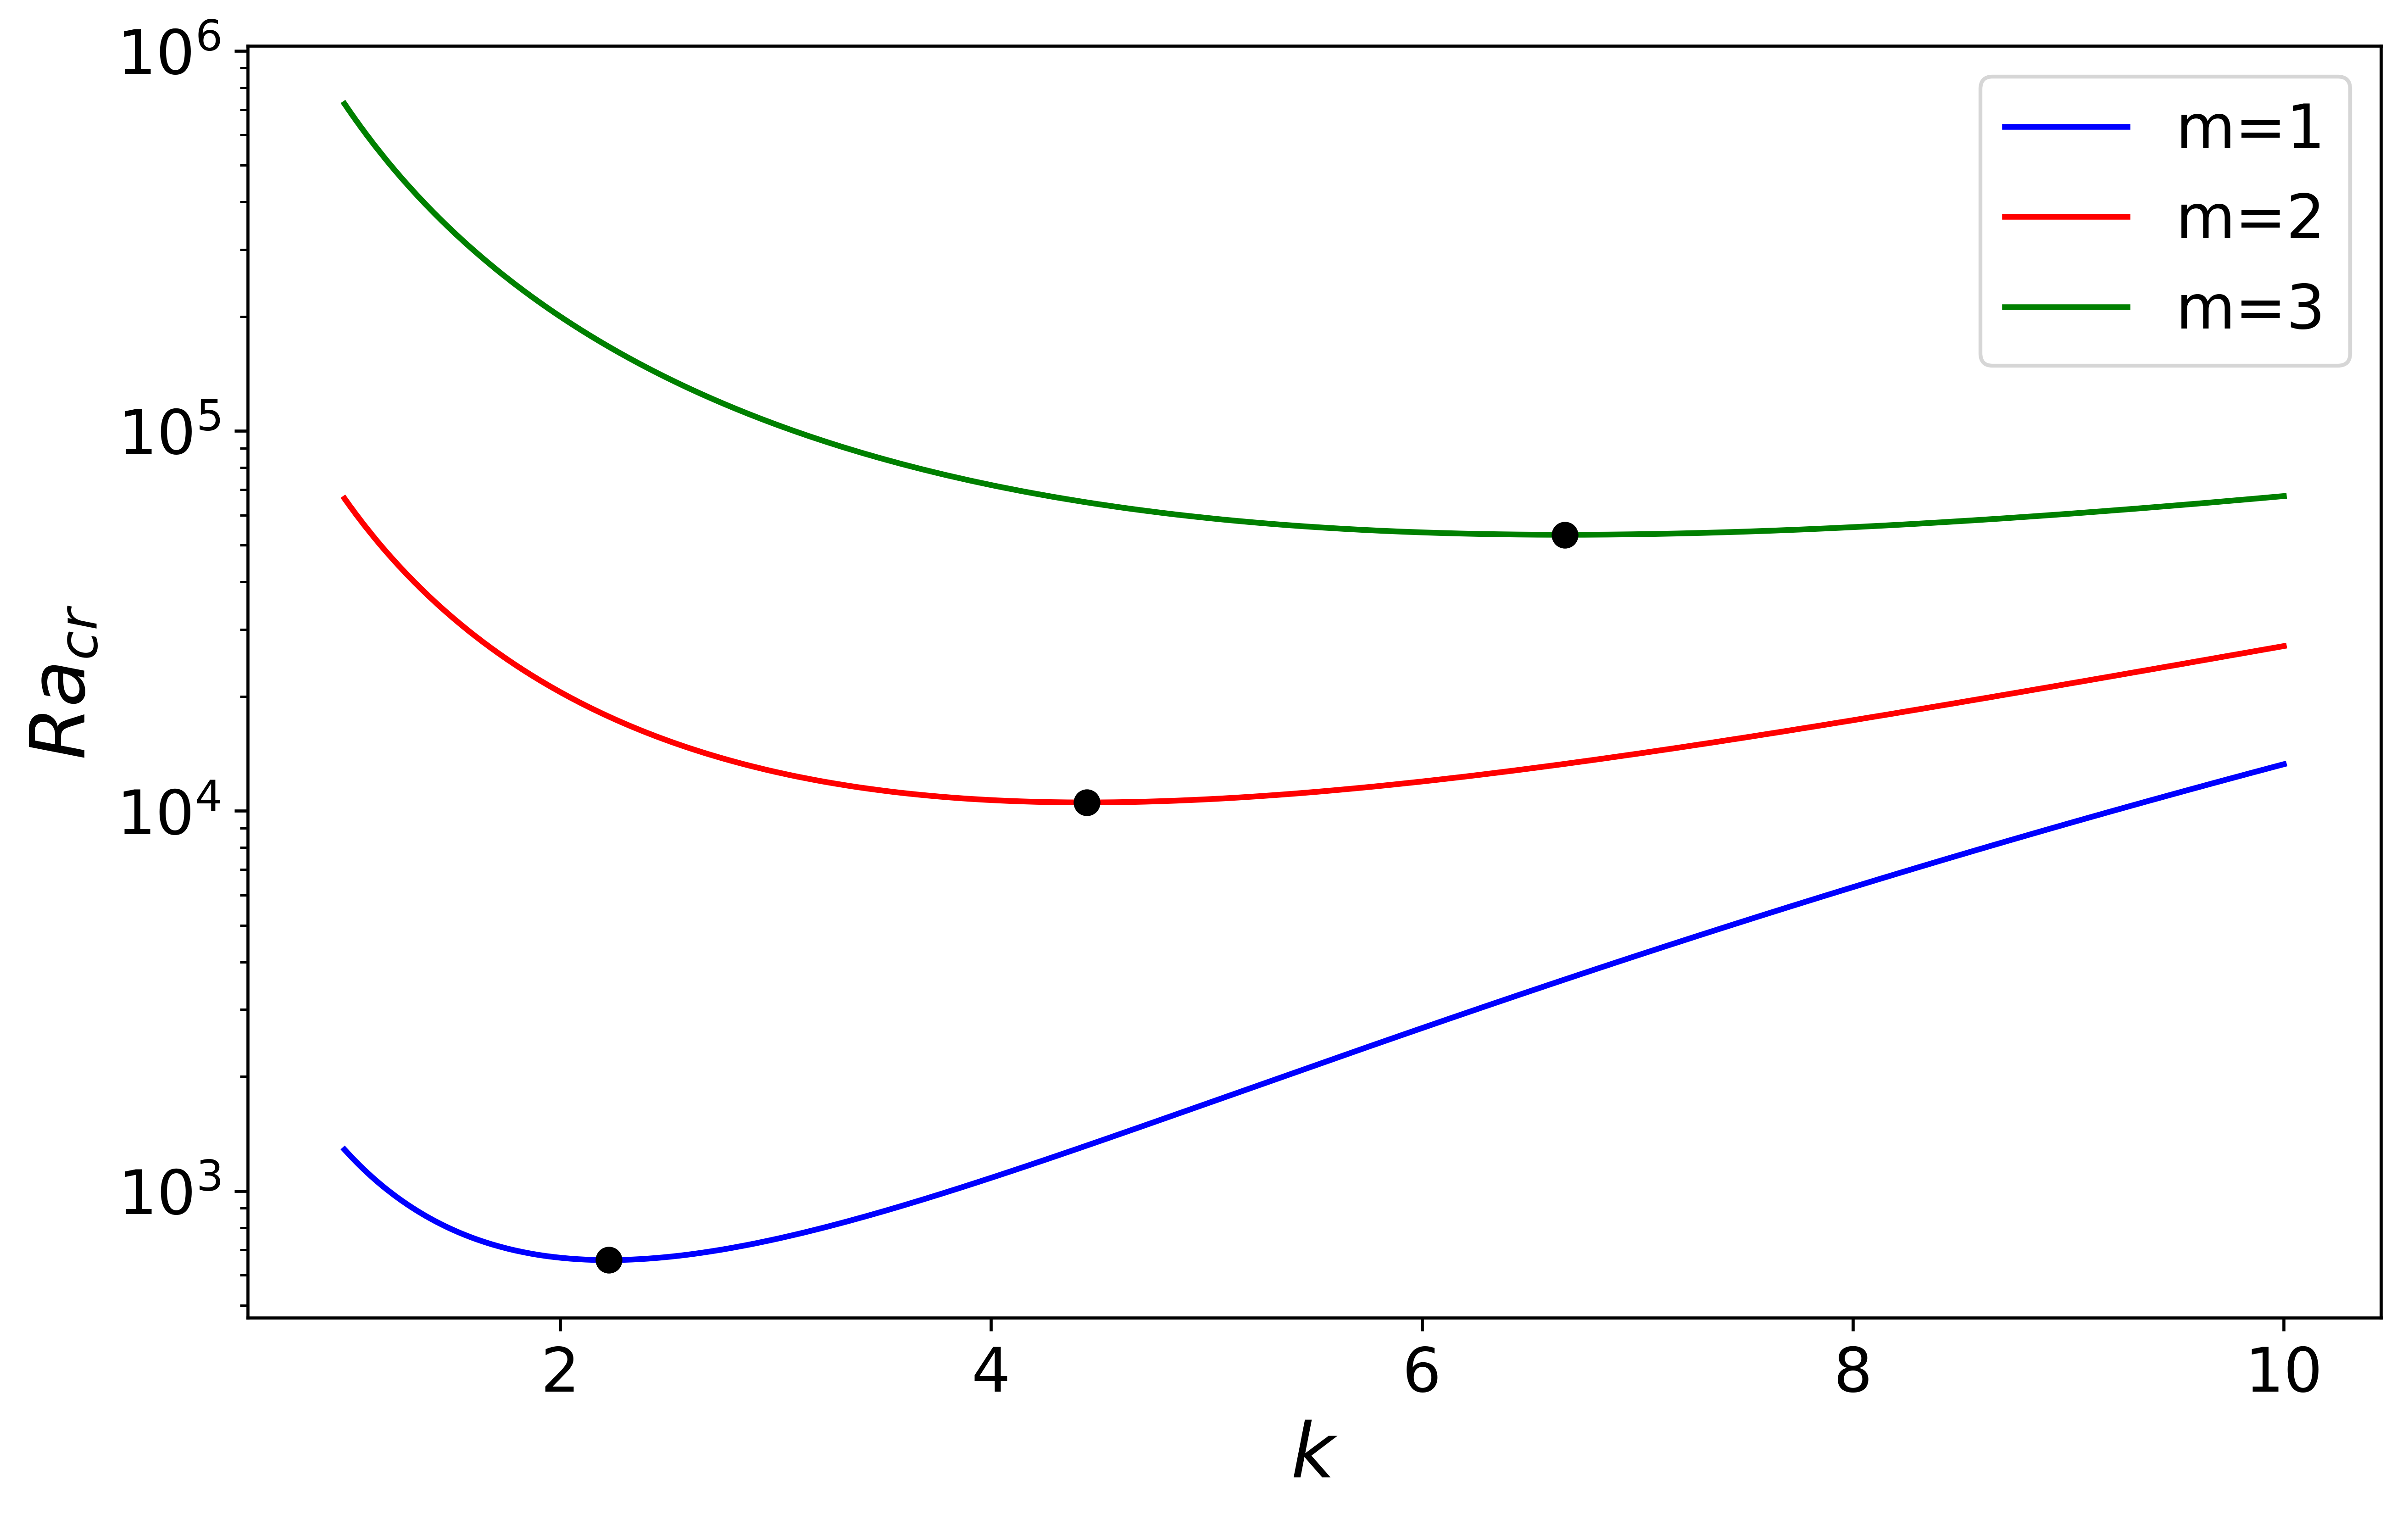
\includegraphics[width=0.7\textwidth]{media/Ra_cr.png}
	\caption{Critical Rayleigh number $Ra_{cr}$ versus wavenumber $k$ for different values of $m$.}
	\label{fig:Ra_cr}
\end{figure}

\noindent Fig. \ref{fig:Ra_cr} shows $Ra_{cr}$ for different modes. The base flow is stable if it is stable for all possible normal modes, i.e. if 

\begin{equation}
	Ra < \min_{k,\,m} Ra_{cr}(k,m)
\end{equation}

\noindent By a simple calculation, it follows that

\begin{equation}
	\min_{k} Ra_{cr}(k,m) = \frac{27}{4}(m \pi)^4
\end{equation}

\noindent Thus the base flow is stable for 

\begin{equation}
	Ra < Ra_{cr} = \frac{27}{4}(\pi)^4 = 657.5
\end{equation}

\noindent which corresponds to the instability threshold of the first vertical mode.

\section{Including Nonlinear Interactions - The Lorenz System}

\subsection{Modeling}
Linear stability analysis does not provide much insight into the flow dynamics beyond the critical Rayleigh number at which the base flow becomes unstable. Thus, we will attempt to reintroduce the nonlinear terms into Eqns. \ref{linearstreamfunctioneqn}-\ref{lineartemperatureeqn}.

We will only consider the least stable mode $(m=1, \, k = \frac{\pi}{\sqrt{2}}, \, \gamma = \frac{3\pi^2}{2})$, since it drives the bifurcation behavior of the system. Let us first consider a general functional form of the sinusoidal horizontal modes for $\psi$. This forces us to consider the cosine horizontal mode for $\theta$.

\begin{equation}
	\psi(x,z,t) = \hat{\psi}(t) \, sin \, kx  \, sin \, \pi z =: \hat{\psi}(t) \, \phi_{k,1}(x,z)
	\label{initpsi}
\end{equation}
\begin{equation}
	\theta(x,z,t) = \hat{\theta}(t) \, cos \, kx  \, sin \, \pi z =: \hat{\theta}(t) \, \varphi_{k,1}(x,z)
	\label{inittheta}
\end{equation}



\noindent Inserting the forms \ref{initpsi}-\ref{inittheta} into the Poisson brackets,

\begin{equation}
	J[\psi, \nabla^2 \psi] = J[\psi, -\gamma^2 \psi] = -\gamma^2 J[\psi, \psi] = 0
\end{equation}
\begin{equation}
	J[\psi, \theta] = \hat{\psi} \, \hat{\theta} \, J[\phi_{k,1}, \varphi_{k,1}] = \hat{\psi} \, \hat{\theta} \, \frac{k \pi}{2} \, sin \, 2 \pi z
\end{equation}

Thus we see that including the nonlinear term $J[\psi, \nabla^2 \psi]$ has no effect, but using the functional form \ref{initpsi}-\ref{inittheta} is inconsistent with the nonlinear term $J[\psi, \theta]$. Let us now further generalize the functional forms to add the $sin \, 2 \pi z$ mode to $\theta$ since it appears in the $\theta$ equation.

\begin{equation}
	\theta(x,z,t) = \hat{\theta_1}(t) \, cos \, kx  \, sin \, \pi z - \hat{\theta_2}(t) \, sin \, 2 \pi z =: \hat{\theta_1}(t) \, \varphi_{k,1}(x,z) - \hat{\theta_2}(t) \, \vartheta_2(z)
	\label{lorenztheta}
\end{equation}

\noindent The nonlinear interaction between $\psi$ and $\theta_2$ is
\begin{equation}
	J[\psi, \theta_2] =  \hat{\psi} \, \hat{\theta_2} \, k \, \pi \, cos \, kx \,\bigl(sin \, \pi z - sin \, 3 \pi z\bigr)
\end{equation}

The mode $cos \, kx  \, sin \, \pi z$ has already been included in the functional form for $\theta$, but the mode $cos \, kx  \, sin \, 3 \pi z$ has not. Introducing this mode would lead to additional terms in the nonlinear interaction resulting in a closure problem. This is reminiscent of the closure problem seen in the modeling of turbulence. \\

Lorenz suggested stopping at $\theta_2$ and neglecting the additional term generated. Substituting \ref{initpsi},\ref{lorenztheta} in \ref{streamfunctioneqn}-\ref{streamfunctiontemperatureeqn} and using the orthogonality of the modes, we get:

\begin{equation}
	\frac{d\hat{\psi}}{d t} = Pr \, \biggl(k \frac{\hat{\theta_1}}{\gamma^2} - \gamma^2 \hat{\psi}\biggr)
	\label{dimlrzx}
\end{equation}
\begin{equation}
	\frac{d\hat{\theta_1}}{d t} = - k\pi \, \hat{\psi} \, \hat{\theta_2} + \, Ra \, k\,  \hat{\psi} - \gamma^2 \hat{\theta_1}
\end{equation}
\begin{equation}
	\frac{d\hat{\theta_2}}{d t} = \frac{k \pi}{2} \, \hat{\psi}\,\hat{\theta_1} - 4 \pi^2  \hat{\theta_2}
\end{equation}

\noindent Defining 
\begin{equation}
	X \equiv \frac{k \pi}{\sqrt{2}\gamma^2} \, \hat{\psi}, \qquad Y \equiv \frac{k^2 \pi}{\sqrt{2}\gamma^6} \hat{\theta_1}, \qquad Z \equiv \frac{k^2 \pi}{\gamma^6} \hat{\theta_2}
	\label{ND1}
\end{equation}

\begin{equation}
	\tau \equiv \gamma^2 t , \qquad r \equiv \frac{Ra}{Ra_{cr}}, \qquad b \equiv \frac{4\pi^2}{\gamma^2} \equiv \frac{8}{3}, \qquad \sigma \equiv Pr
	\label{ND2}
\end{equation}

\noindent gives us the famous Lorenz system:

\begin{equation}
	\dot{X} = \sigma \, (Y-X)
	\label{lrzx}
\end{equation}
\begin{equation}
	\dot{Y} = -X\,Z + r\,X - Y
	\label{lrzy}
\end{equation}
\begin{equation}
	\dot{Z} = X\,Y-b\,Z
	\label{lrzz}
\end{equation}

The physical origin of each term in the equations is clear. The quadratic terms result from nonlinear interactions between temperature and momentum, the negative linear terms represent viscous and thermal dissipation, and the remaining cross-linear terms capture the effects of buoyancy. As expected, the system is dissipative, with the divergence of the vector field given by 
\begin{equation} 
	\frac{\partial \dot{X}}{\partial X} + \frac{\partial \dot{Y}}{\partial Y} + \frac{\partial \dot{Z}}{\partial Z} = - (\sigma + b + 1). 
\end{equation}

\subsection{Bifurcation Analysis}
We will consider the parameters used by Lorenz for our analysis, i.e. $\sigma = 10$ which roughly corresponds to the Prandtl number of water. The parameter $r$ is the Rayleigh number divided by its threshold, and will be the control parameter. \\

\noindent Steady states of Eqns. \ref{lrzx}-\ref{lrzz} satisfy 

\begin{equation}
	0 = \sigma (Y-X) \Rightarrow X = Y
\end{equation}
\begin{equation}
	0 = - X \, Z + r \, X - Y \Rightarrow X = 0 \text{ or } Z = r - 1
\end{equation}
\begin{equation}
	0 = X \, Y - b \, Z \Rightarrow Z = 0 \text{ or } X = Y = \pm \sqrt{b(r-1)}
\end{equation}

\noindent The steady states are therefore $(0,0,0)$ and $(\pm \sqrt{b(r-1)}, \pm \sqrt{b(r-1)}, r-1)$.\\

\noindent The Jacobian matrix is given by 
\begin{equation}
	J =
	\begin{bmatrix}
		-\sigma & \sigma & 0 \\
		r - Z & -1 & -X \\
		Y & X & -b
	\end{bmatrix}
\end{equation}

\noindent For $r \leq 1$, the base state $(0,0,0)$ is the only fixed point. The Jacobian for this state is given by 
\begin{equation}
	J =
	\begin{bmatrix}
		-\sigma & \sigma & 0 \\
		r  & -1 & 0 \\
		0 & 0 & -b
	\end{bmatrix}
	\label{jacBase}
\end{equation}

\noindent Since matrix \ref{jacBase} is block diagonal, it's eigenvalues are such that 
\begin{equation}
	\lambda_1 + \lambda_2 = - (\sigma + 1) < 0
\end{equation}
\begin{equation}
	\lambda_1 \lambda_2 = \sigma (1-r) < 0
\end{equation}
\begin{equation}
	\lambda_3 = -b < 0
\end{equation}


\begin{figure}[hbt!]
	\centering
	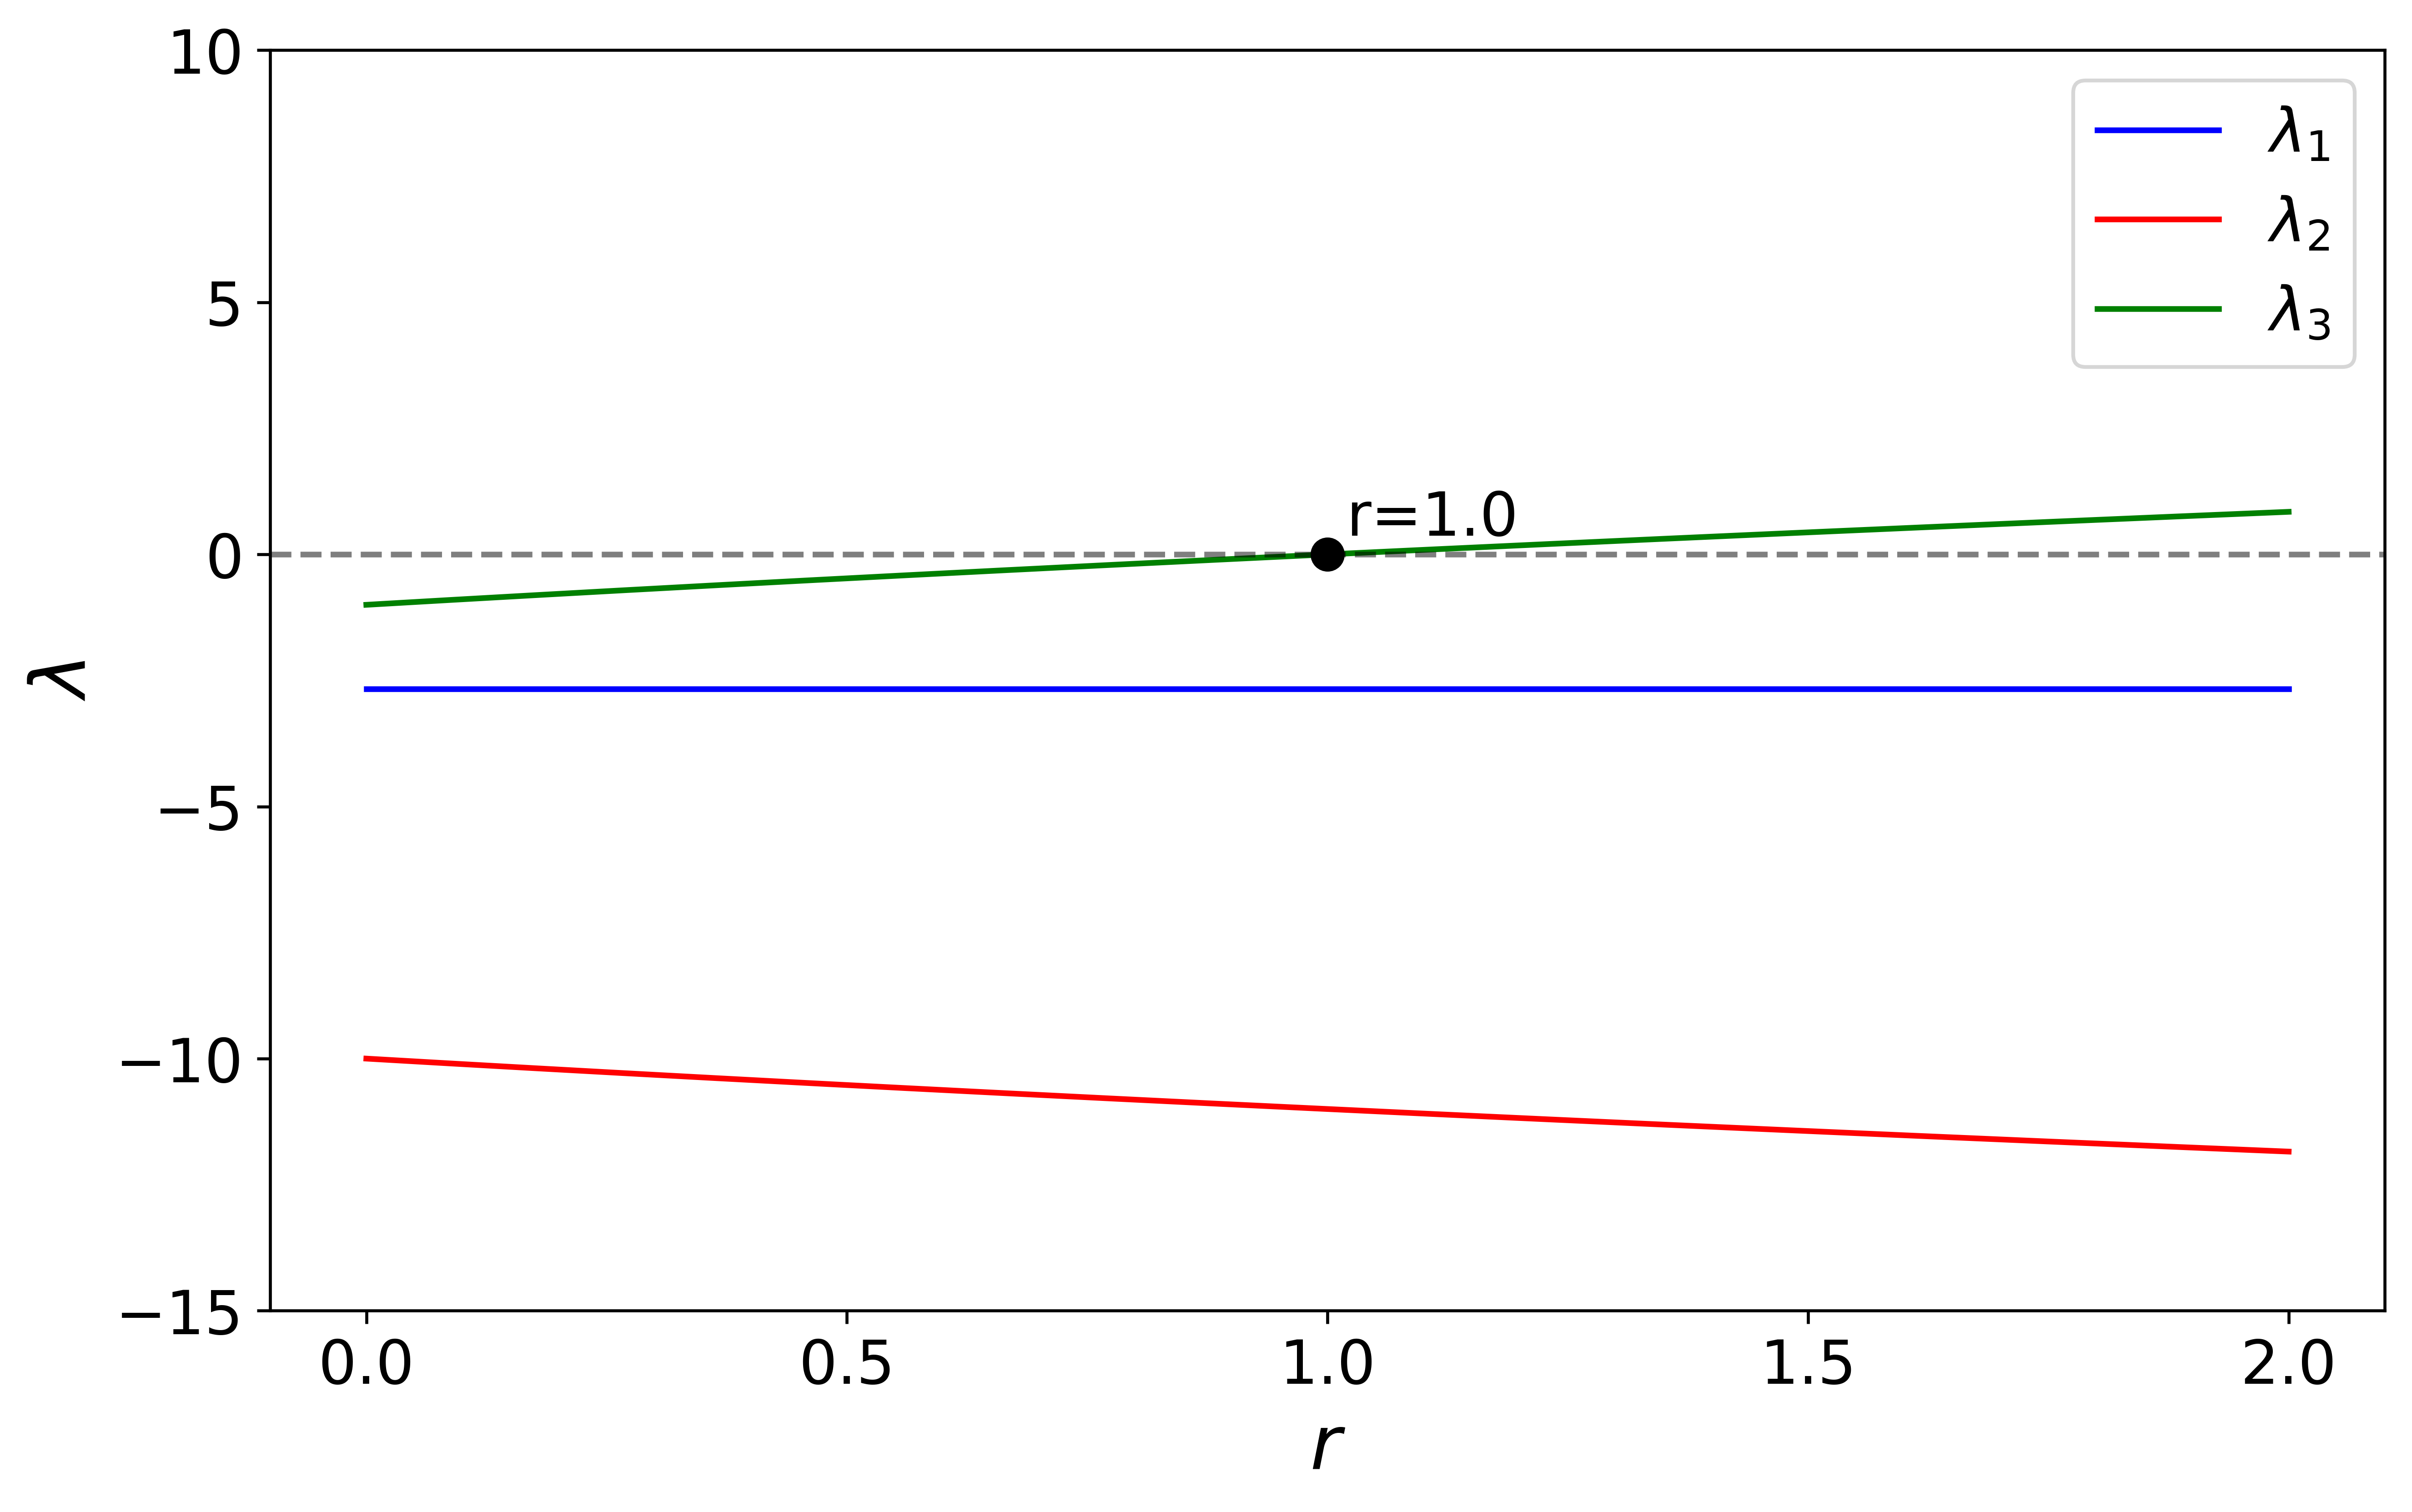
\includegraphics[width=0.7\textwidth]{media/pitchfork_eigs.png}
	\caption{Eigenvalues of the fixed point at the origin versus the parameter $r$.}
	\label{fig:origineigs}
\end{figure}

Figure \ref{fig:origineigs} shows how the eigenvalues at the origin vary with $r$. The base state is a stable node for $r < 1$, and becomes a saddle for $r > 1$. This was also observed in the linear stability analysis performed in the previous section. At $r = 1$, two new fixed points are generated at $(\pm \sqrt{b(r-1)}, \pm \sqrt{b(r-1)}, r-1)$. Thus, a supercritical pitchfork bifurcation occurs at $r=1$. \\

\begin{figure}[hbt!]
	\centering
	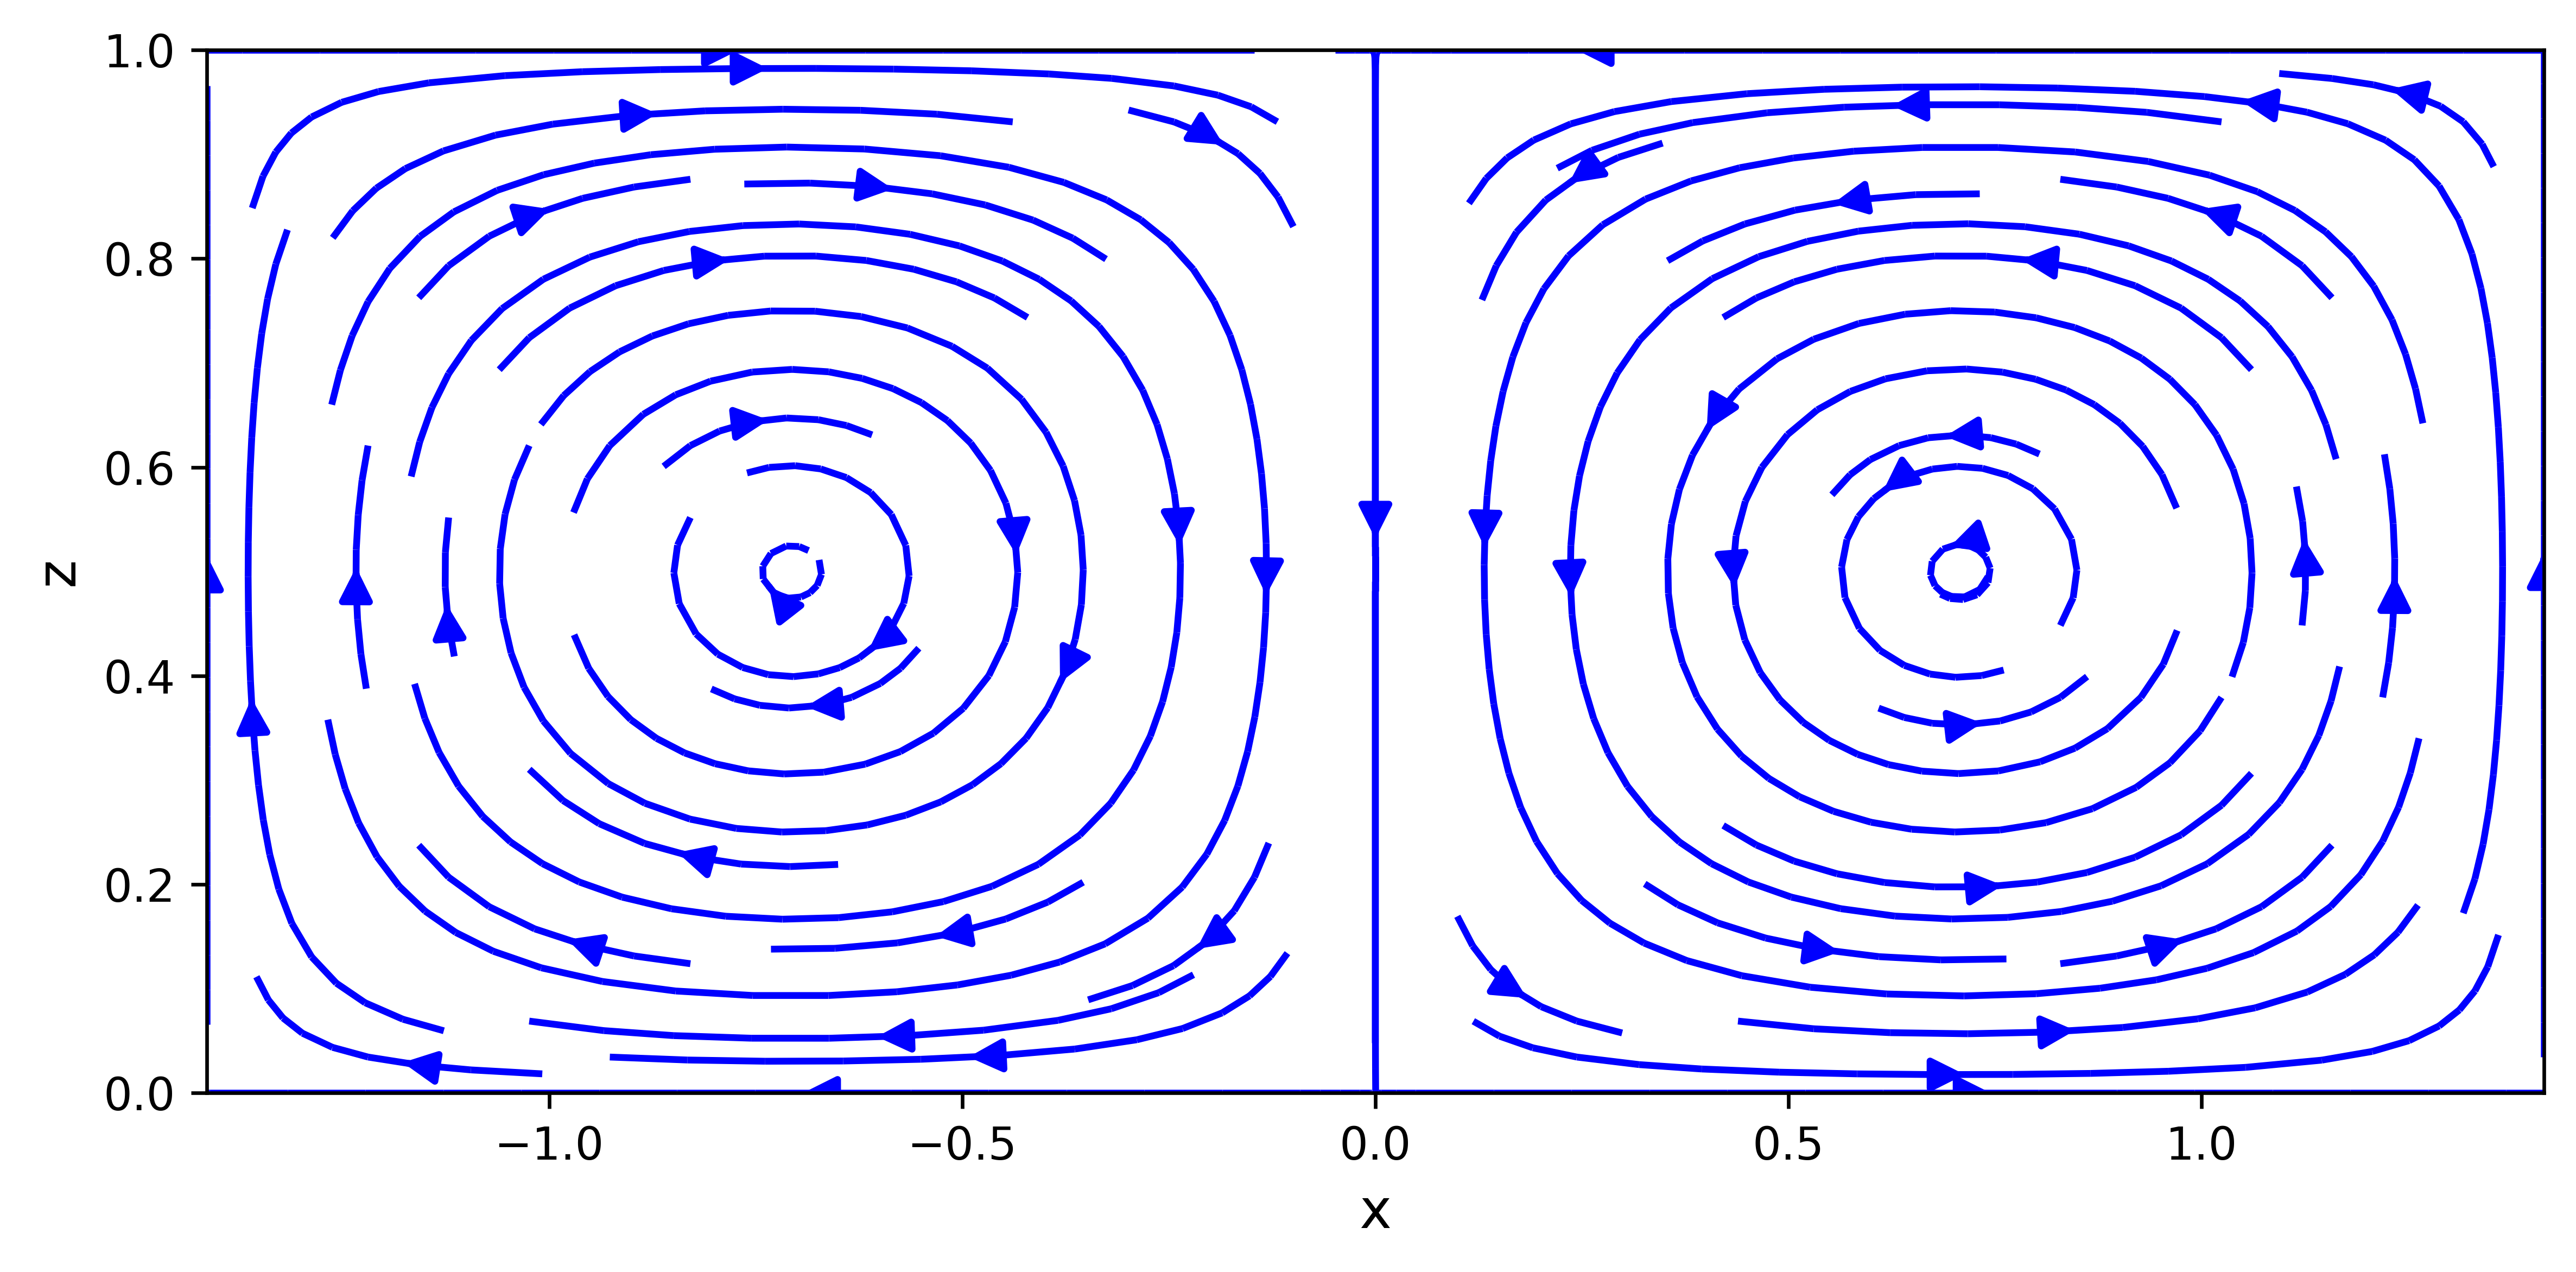
\includegraphics[width=0.9\textwidth]{media/streamlines.png}
	\caption{Streamlines for $\psi = sin \, kx \, sin \, \pi z$}
	\label{fig:streamlines}
\end{figure}

\noindent The two new fixed points correspond to the stream function 
\begin{equation}
	\psi(x,z,t) = \hat{\psi} \, sin \, kx \, sin \, \pi z, \quad \hat{\psi} = constant
\end{equation}
This results in a configuration characterized by steady counter-rotating convection rolls, as illustrated in Figure \ref{fig:streamlines}. The two symmetric fixed points represent opposite sense of rotation.\\

\noindent The Jacobian at these fixed points is given by 
\begin{equation}
	J =
	\begin{bmatrix}
		-\sigma & \sigma & 0 \\
		1 & -1 & \mp \sqrt{b(r-1)} \\
		\pm \sqrt{b(r-1)} & \pm \sqrt{b(r-1)} & -b
	\end{bmatrix}
\end{equation}
whose eigenvalues are roots of the cubic equation
\begin{equation}
	\lambda^3 + (\sigma + b + 1)\lambda^2 + (r + \sigma) \lambda + 2b\sigma(r-1) = 0
\end{equation}

\begin{figure}[hbt!]
	\centering
	
	\begin{subfigure}[b]{0.49\textwidth}
		\centering
		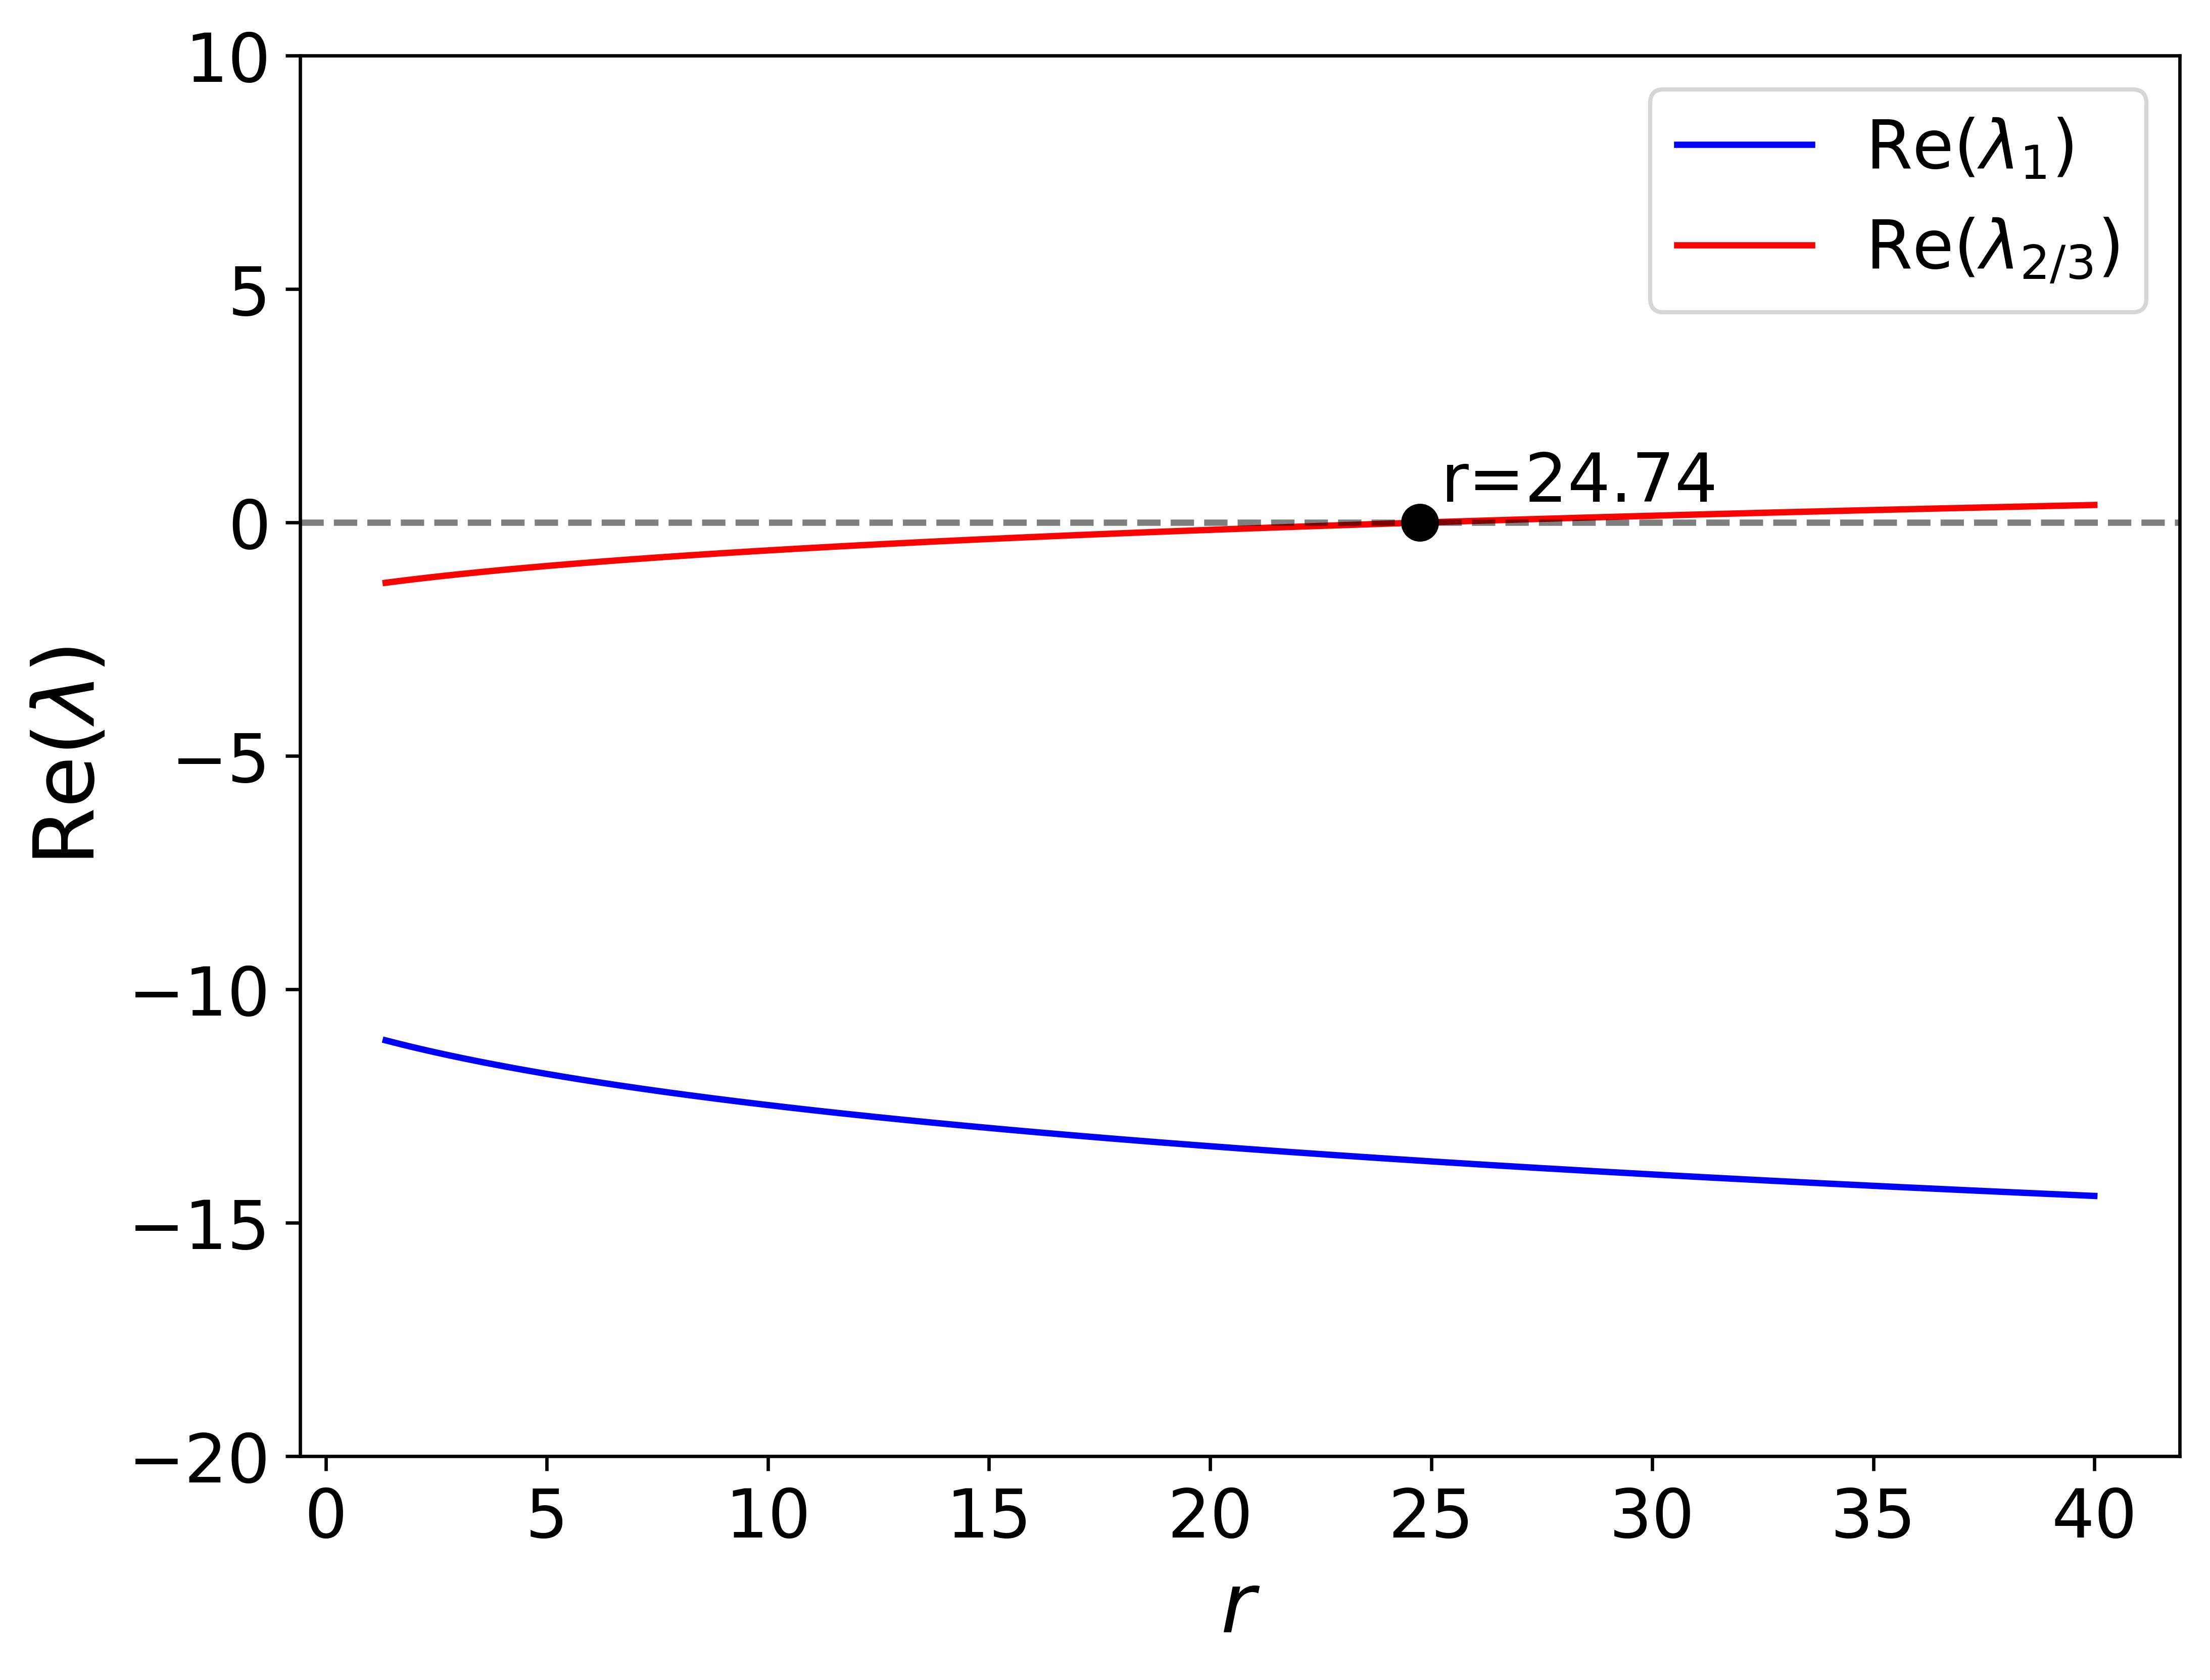
\includegraphics[width=\textwidth]{media/hopf_eigs_real.png}
		\caption{}
		\label{fig:sub1}
	\end{subfigure}
	\hfill
	\begin{subfigure}[b]{0.49\textwidth}
		\centering
		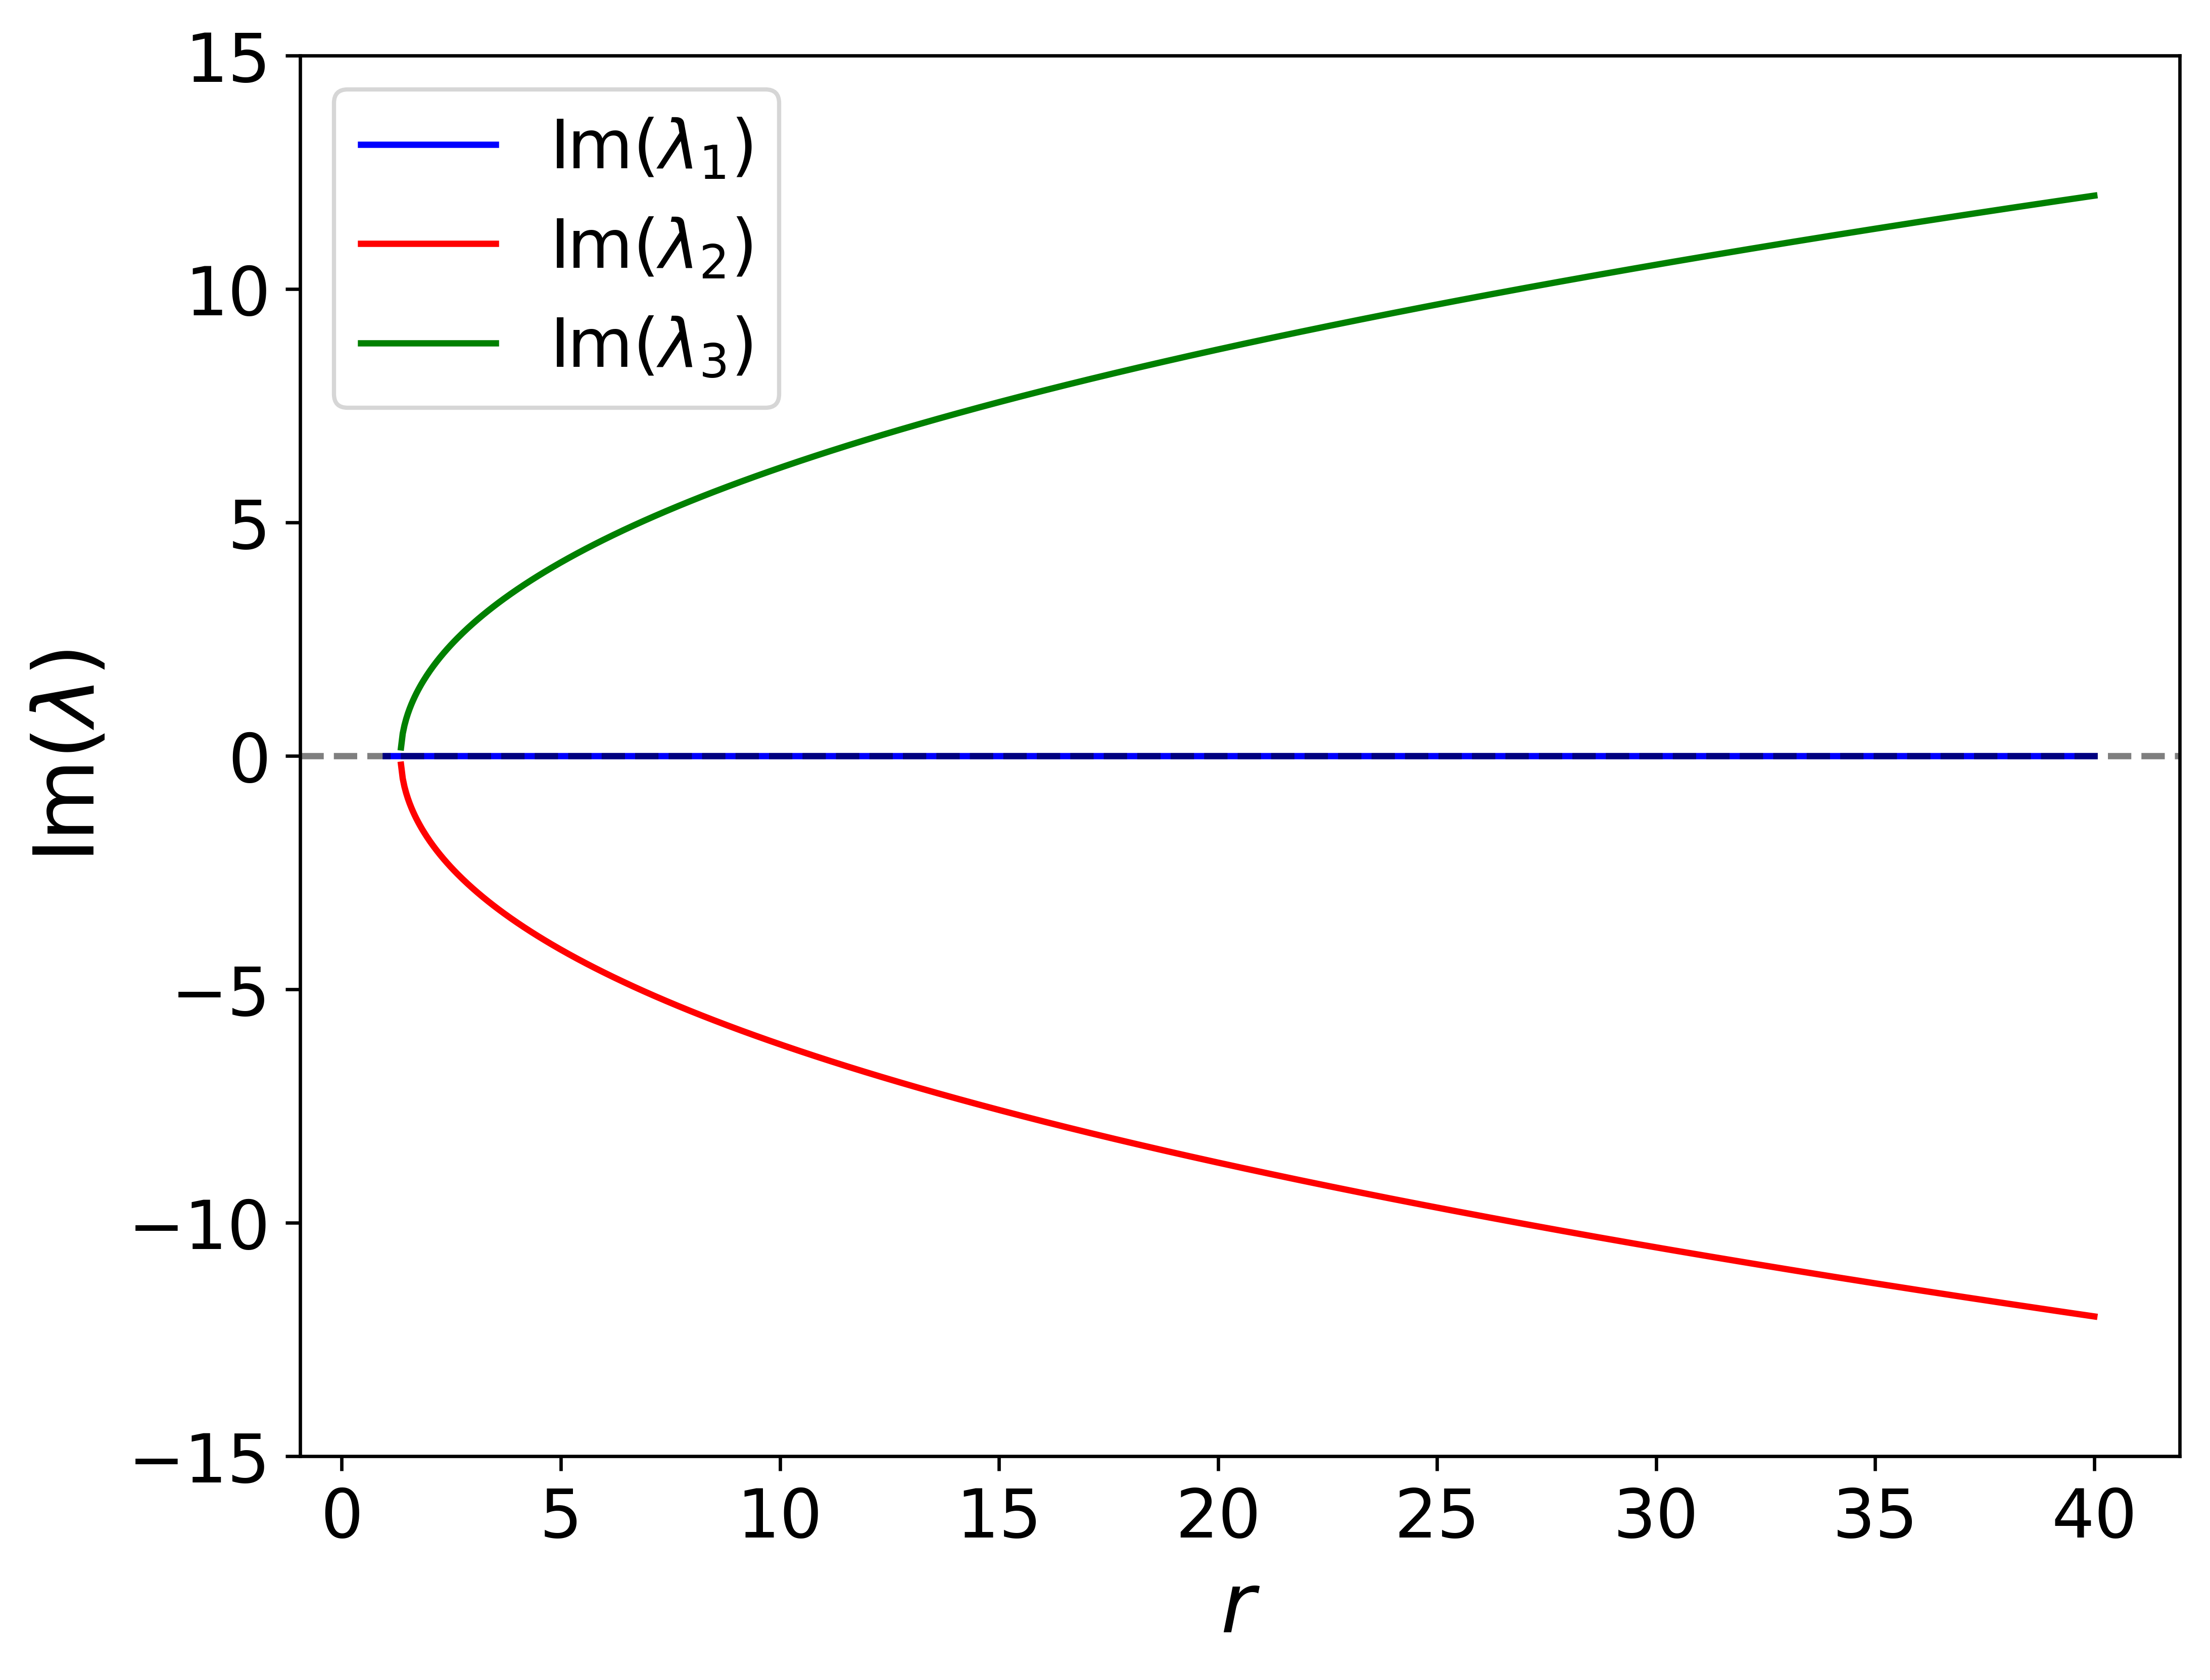
\includegraphics[width=\textwidth]{media/hopf_eigs_imag.png}
		\caption{}
		\label{fig:sub2}
	\end{subfigure}
	
	\caption{Real and imaginary parts of the eigenvalues of the fixed points at $(X,Y,Z) = (\pm\sqrt{b(r-1)},\pm\sqrt{b(r-1)},r-1)$ versus the parameter $r$.}
	\label{fig:hopf_eigs}
\end{figure}

Figure \ref{fig:hopf_eigs} shows how the real and imaginary parts of the eigenvalues vary with the parameter $r$. For $1 < r < 24.74$, the steady convective rolls are stable, and nearby trajectories are attracted to these fixed points. At $r \approx 24.74$, the complex conjugate pair of eigenvalues crosses into the right half-plane, resulting in a Hopf bifurcation. Bifurcation analysis using numerical continuation in AUTO07p, shown in Figure \ref{fig:bifdiag}, reveals that this is a subcritical Hopf bifurcation. Unstable limit cycles exist for $r < 24.74$, and for $r > 24.74$, the state of steady convection becomes unstable and the flow becomes aperiodic.\\

\begin{figure}[hbt!]
	\centering
	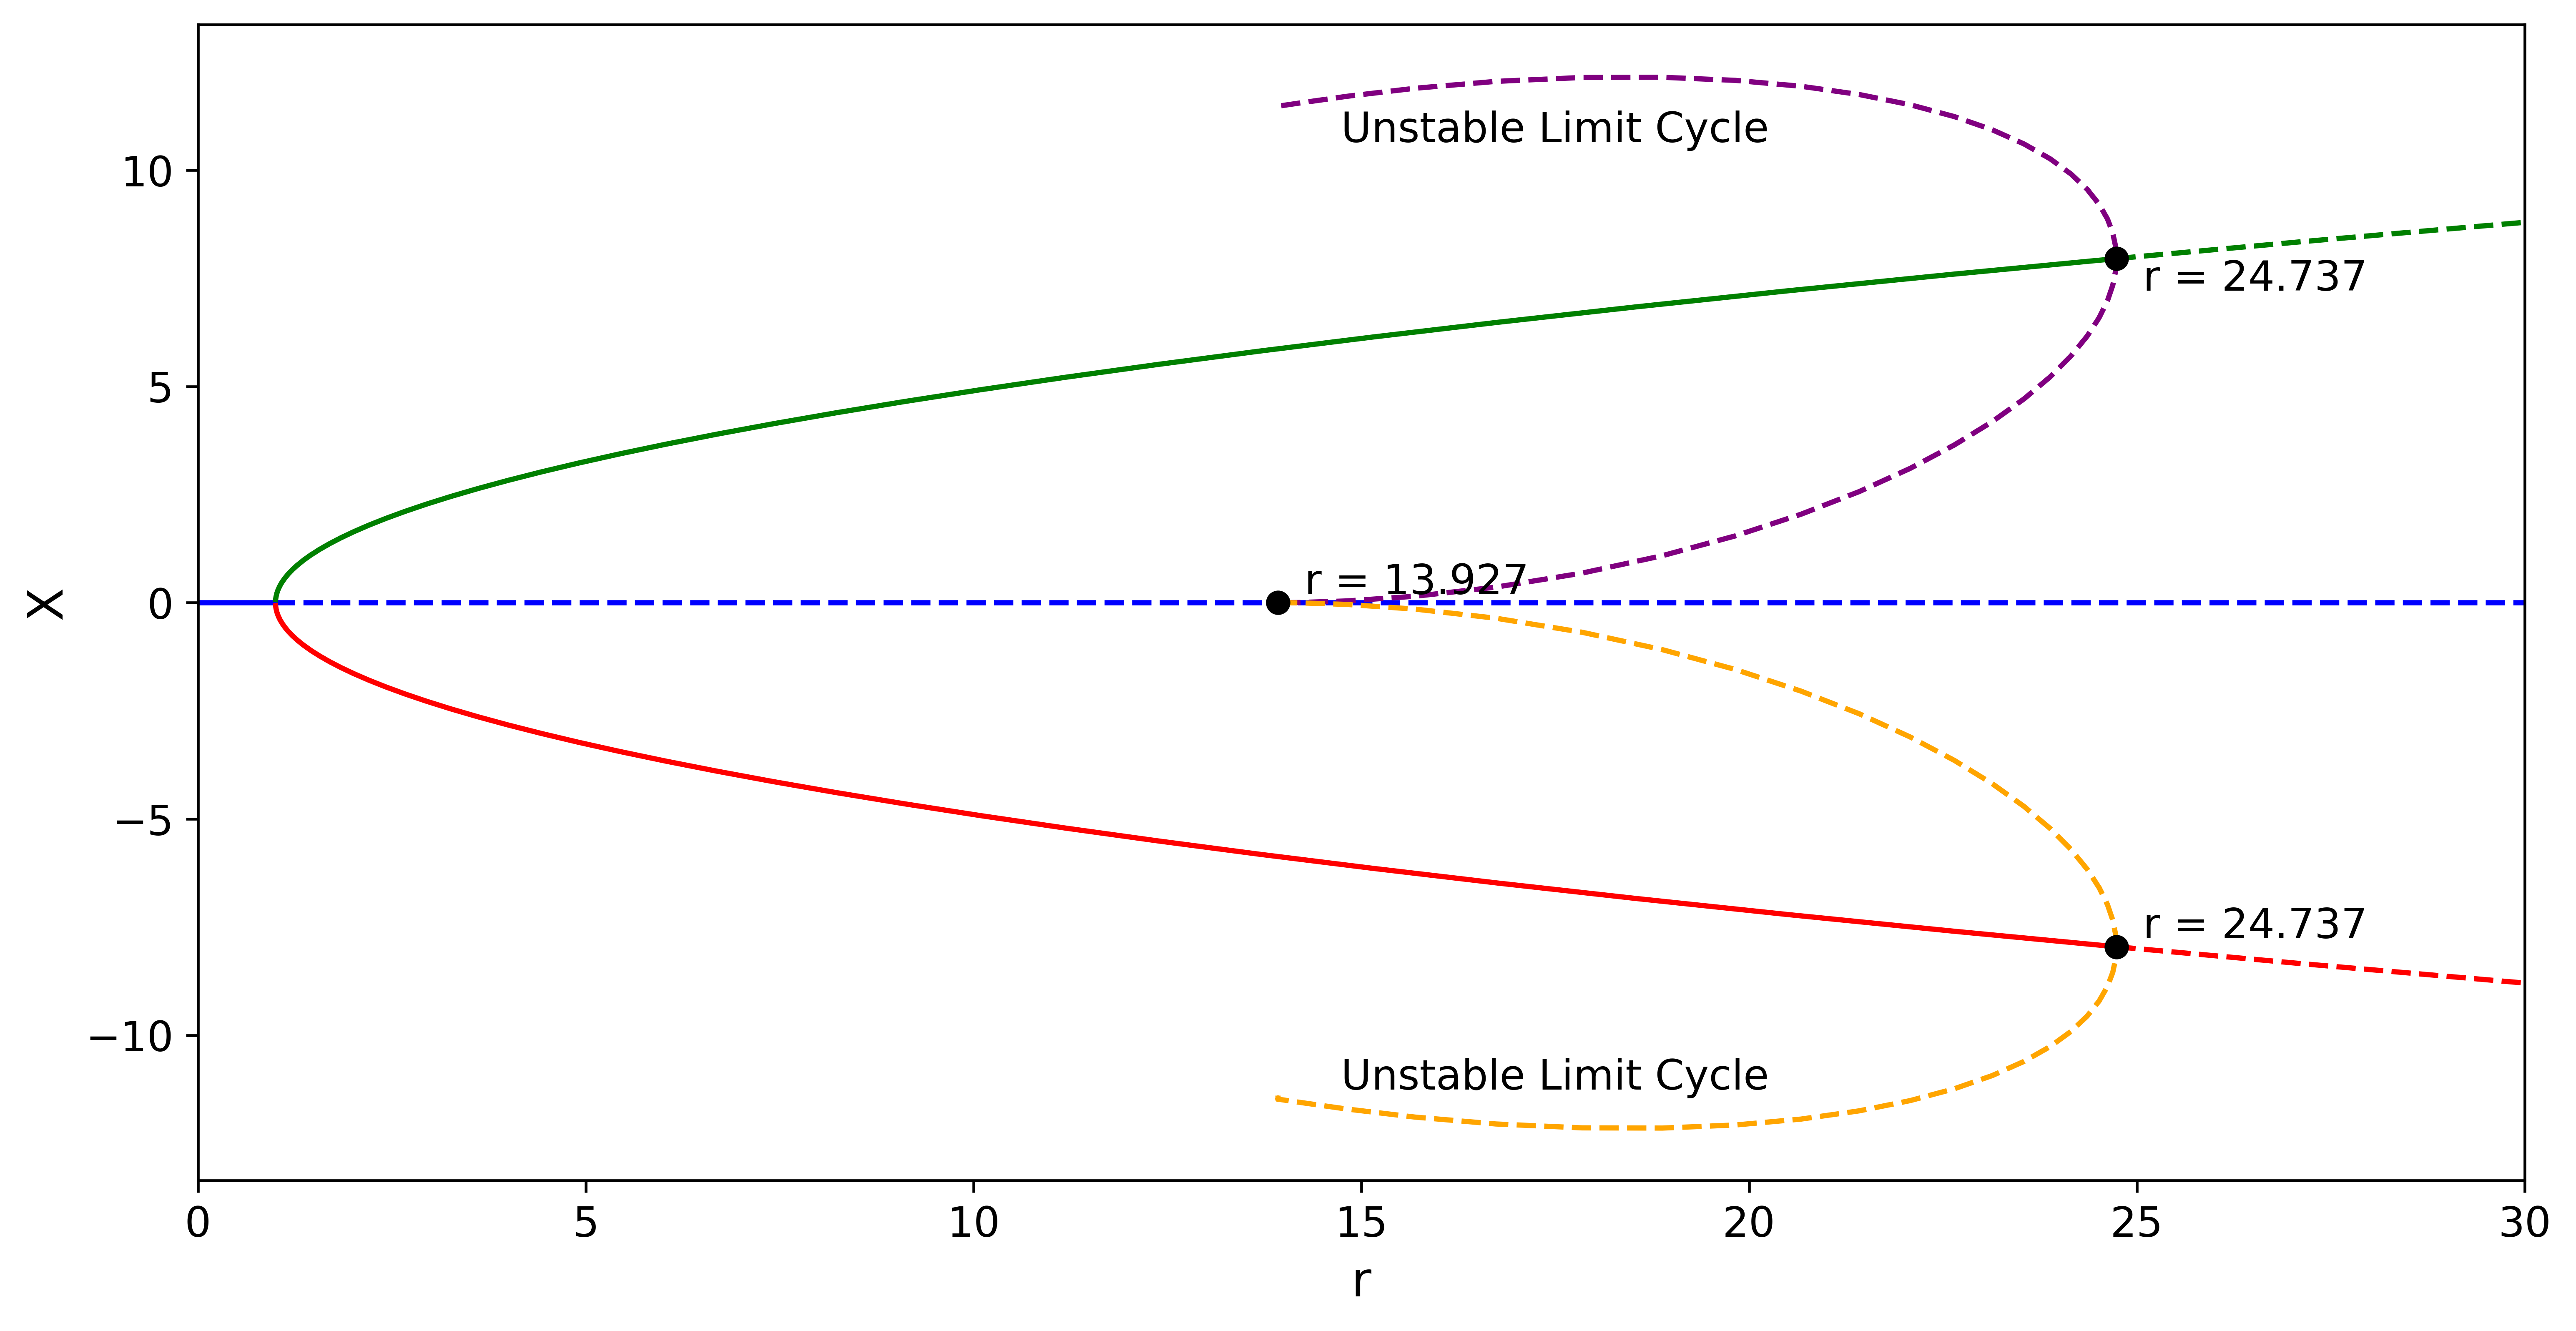
\includegraphics[width=0.9\textwidth]{media/bifurcation_diagram.png}
	\caption{Bifurcation diagram for the Lorenz System. Branches for the limit cycles indicate the minimum and maximum values of $X$ over a period.}
	\label{fig:bifdiag}
\end{figure}

\begin{figure}[hbt!]
	\centering
	
	\begin{subfigure}[b]{0.495\textwidth}
		\centering
		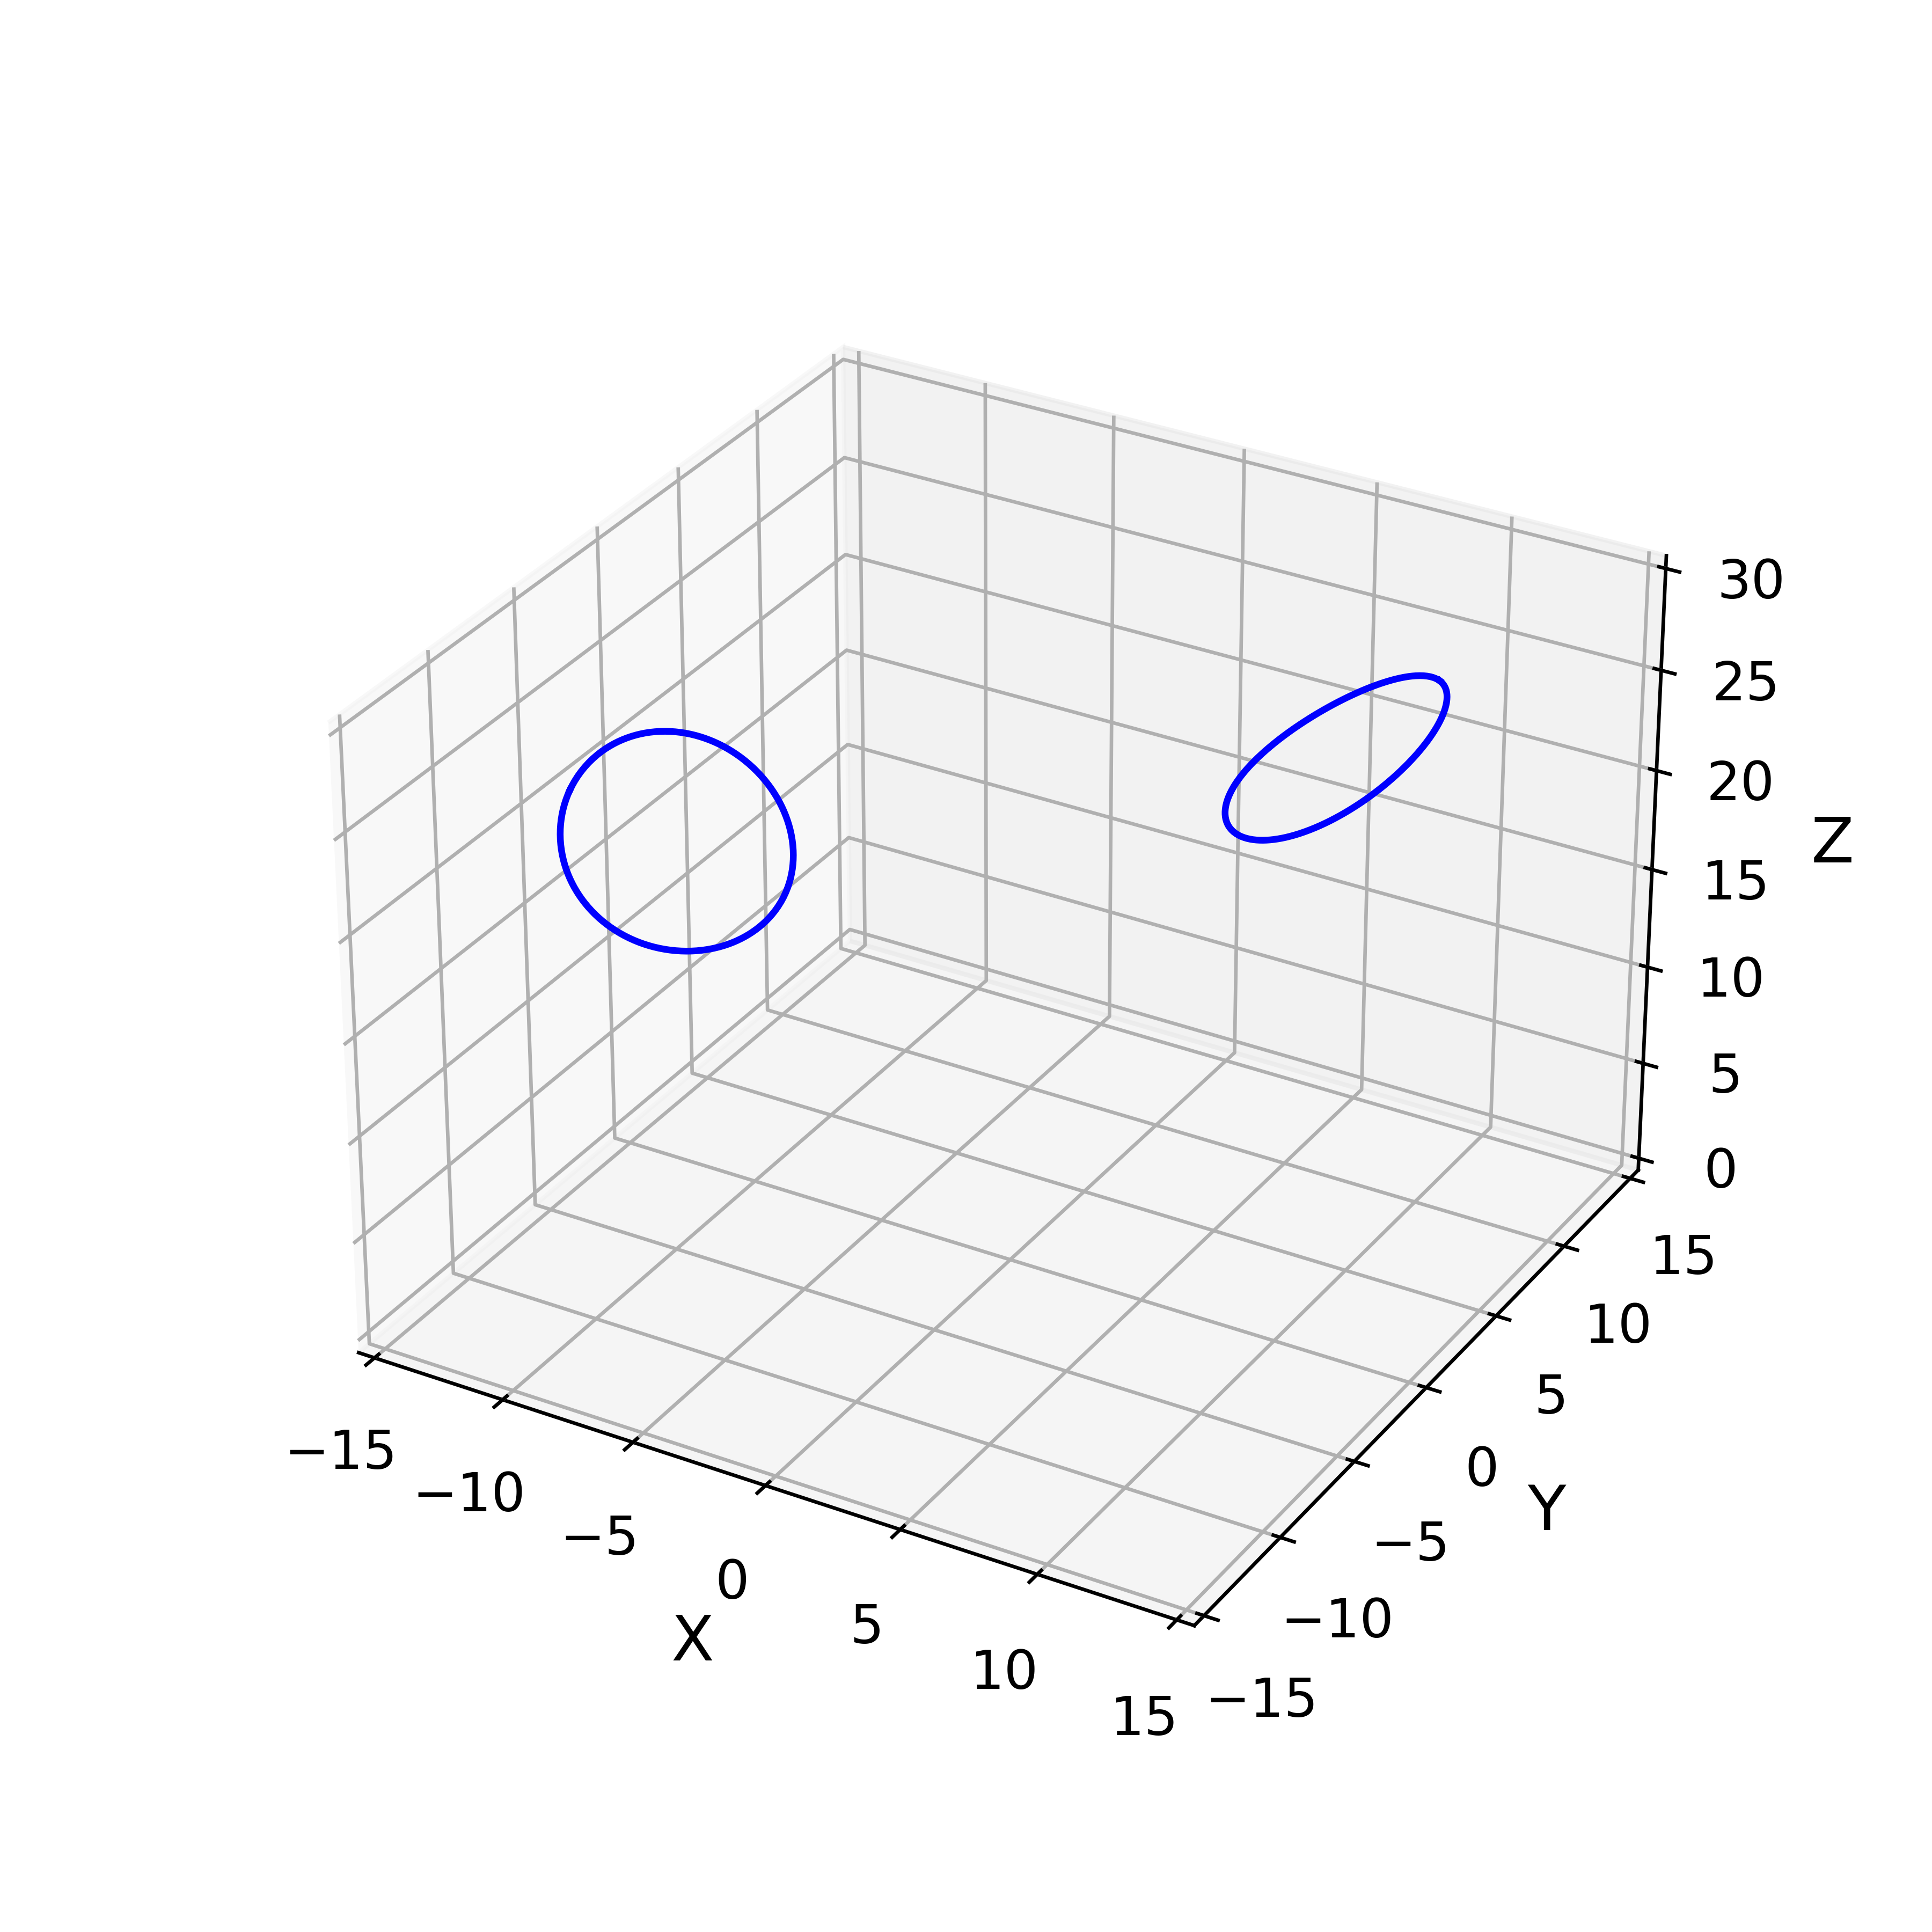
\includegraphics[width=\textwidth]{media/orbit_r_23.88.png}
		\caption{$r = 23.88$}
		\label{fig:sub1}
	\end{subfigure}
	\hfill
	\begin{subfigure}[b]{0.495\textwidth}
		\centering
		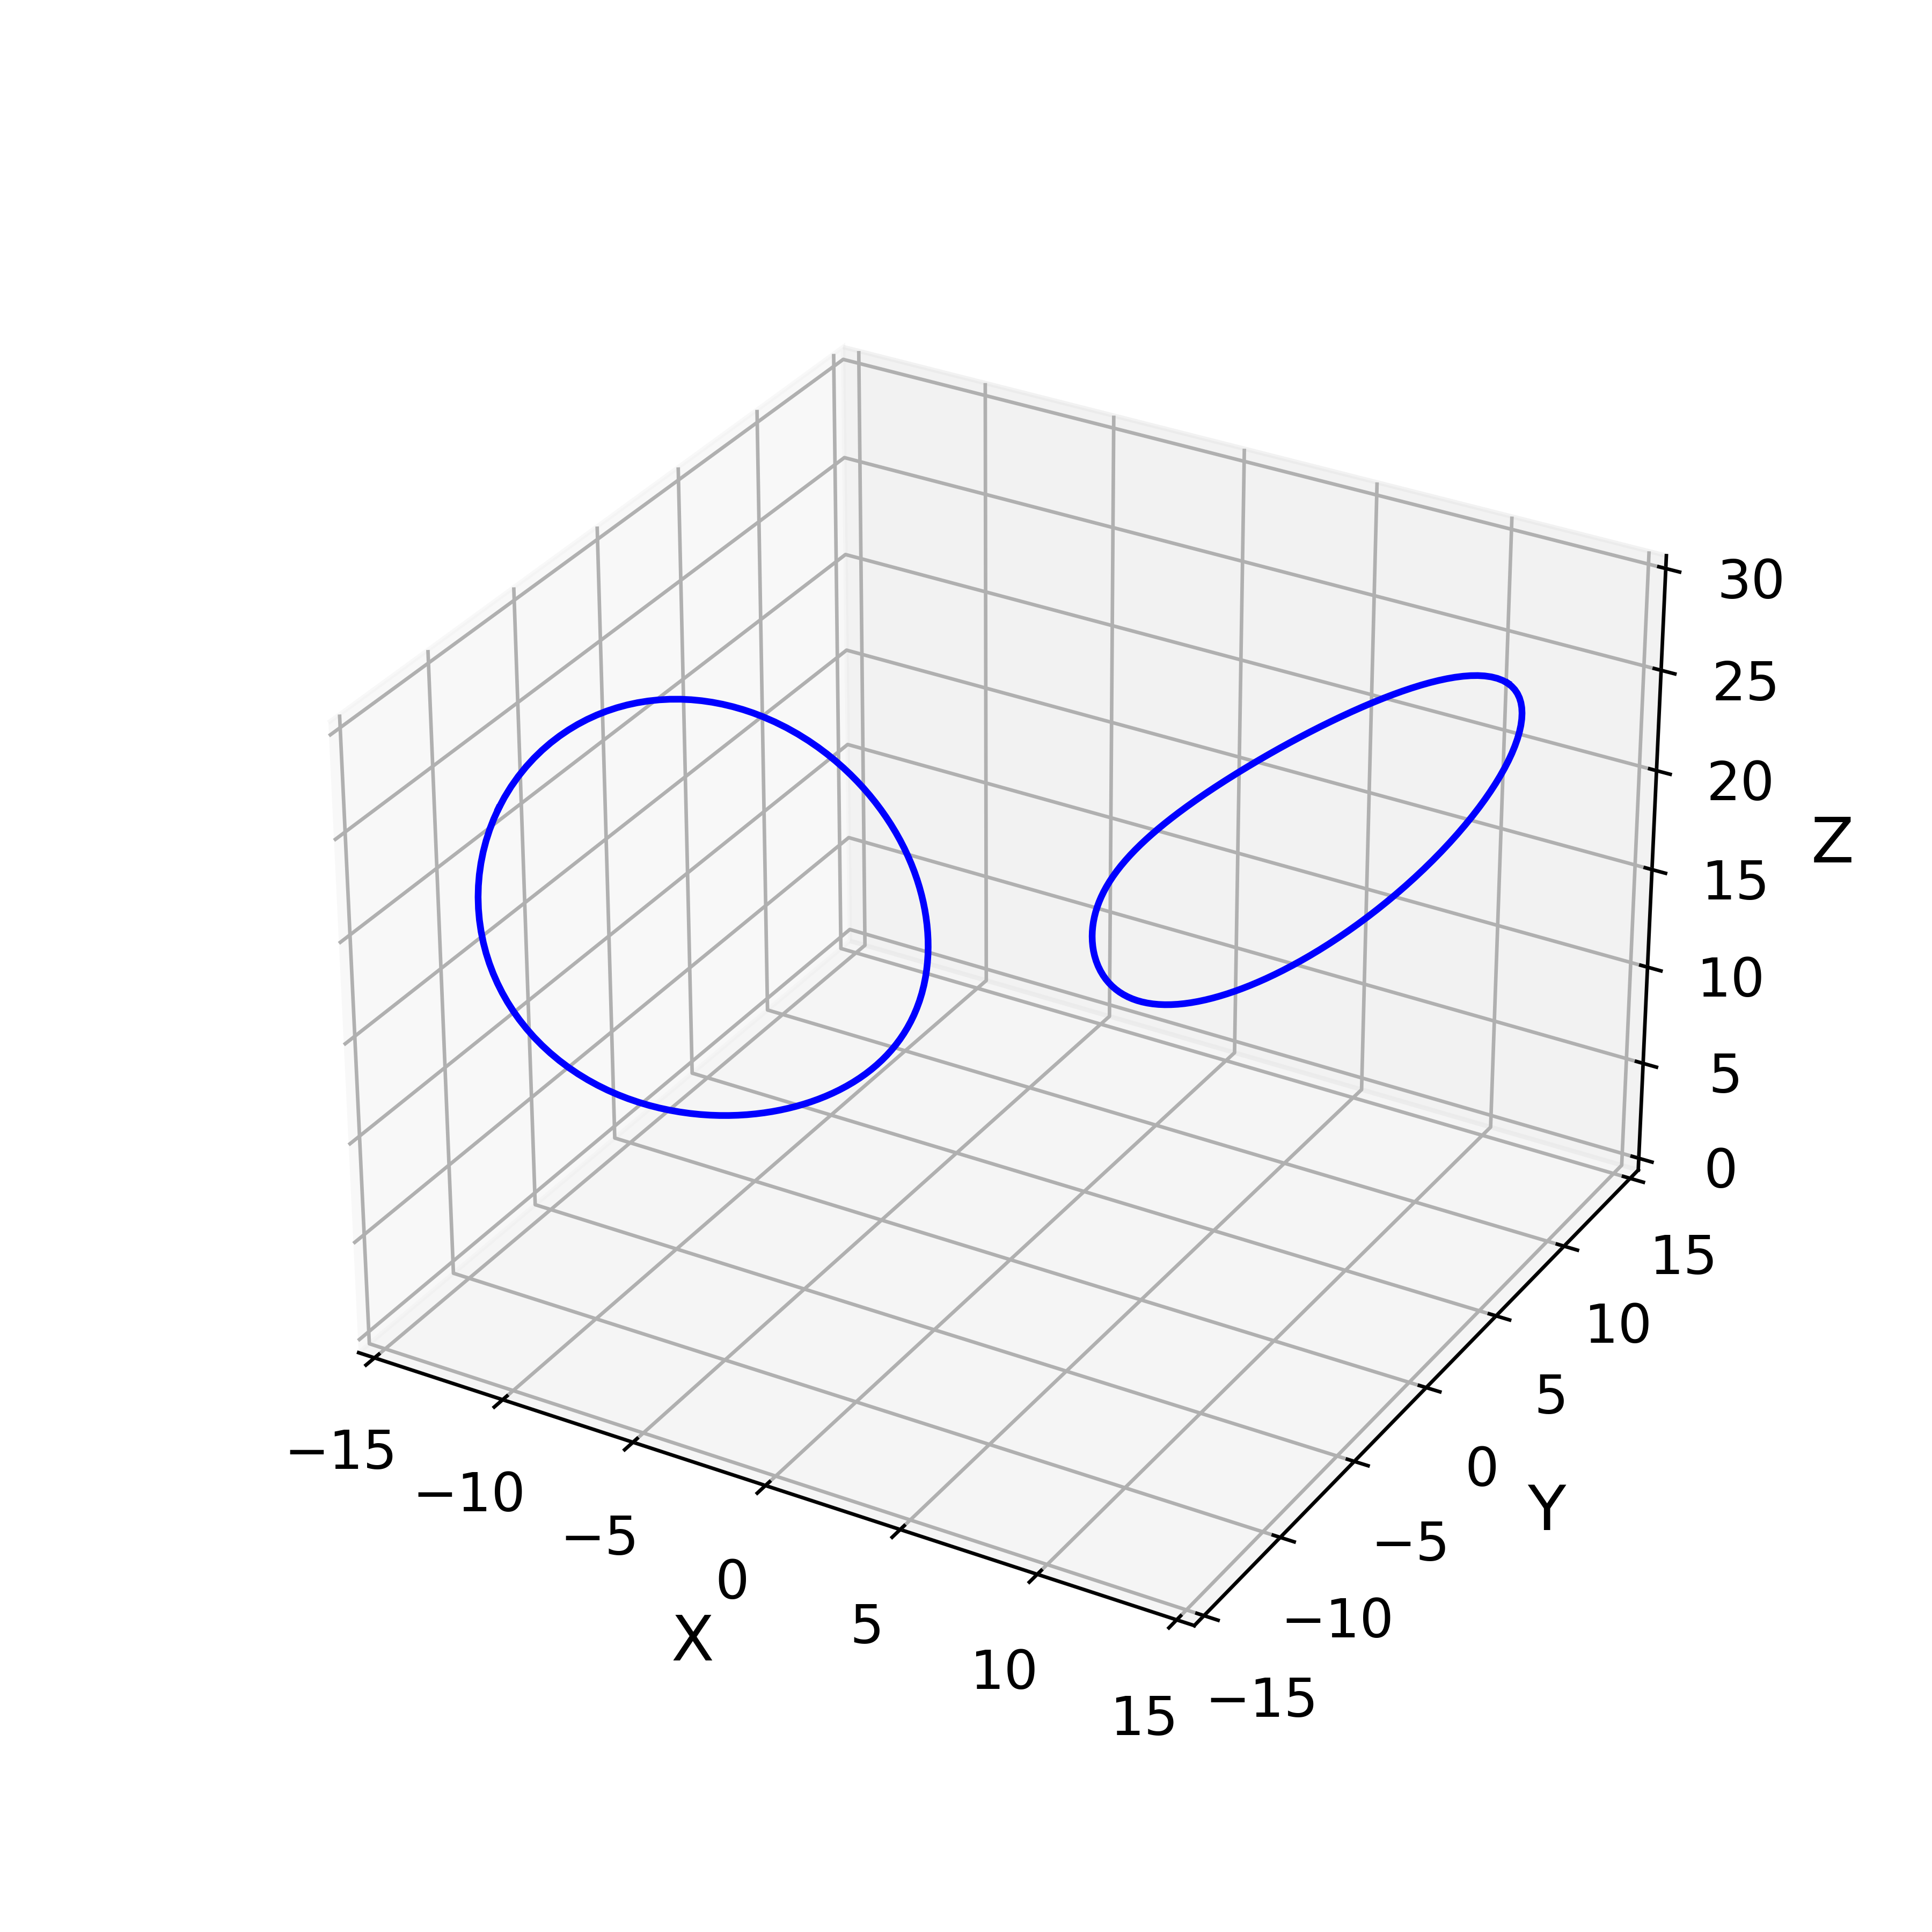
\includegraphics[width=\textwidth]{media/orbit_r_20.67.png}
		\caption{$r = 20.67$}
		\label{fig:sub2}
	\end{subfigure}
	\hfill
	\begin{subfigure}[b]{0.495\textwidth}
		\centering
		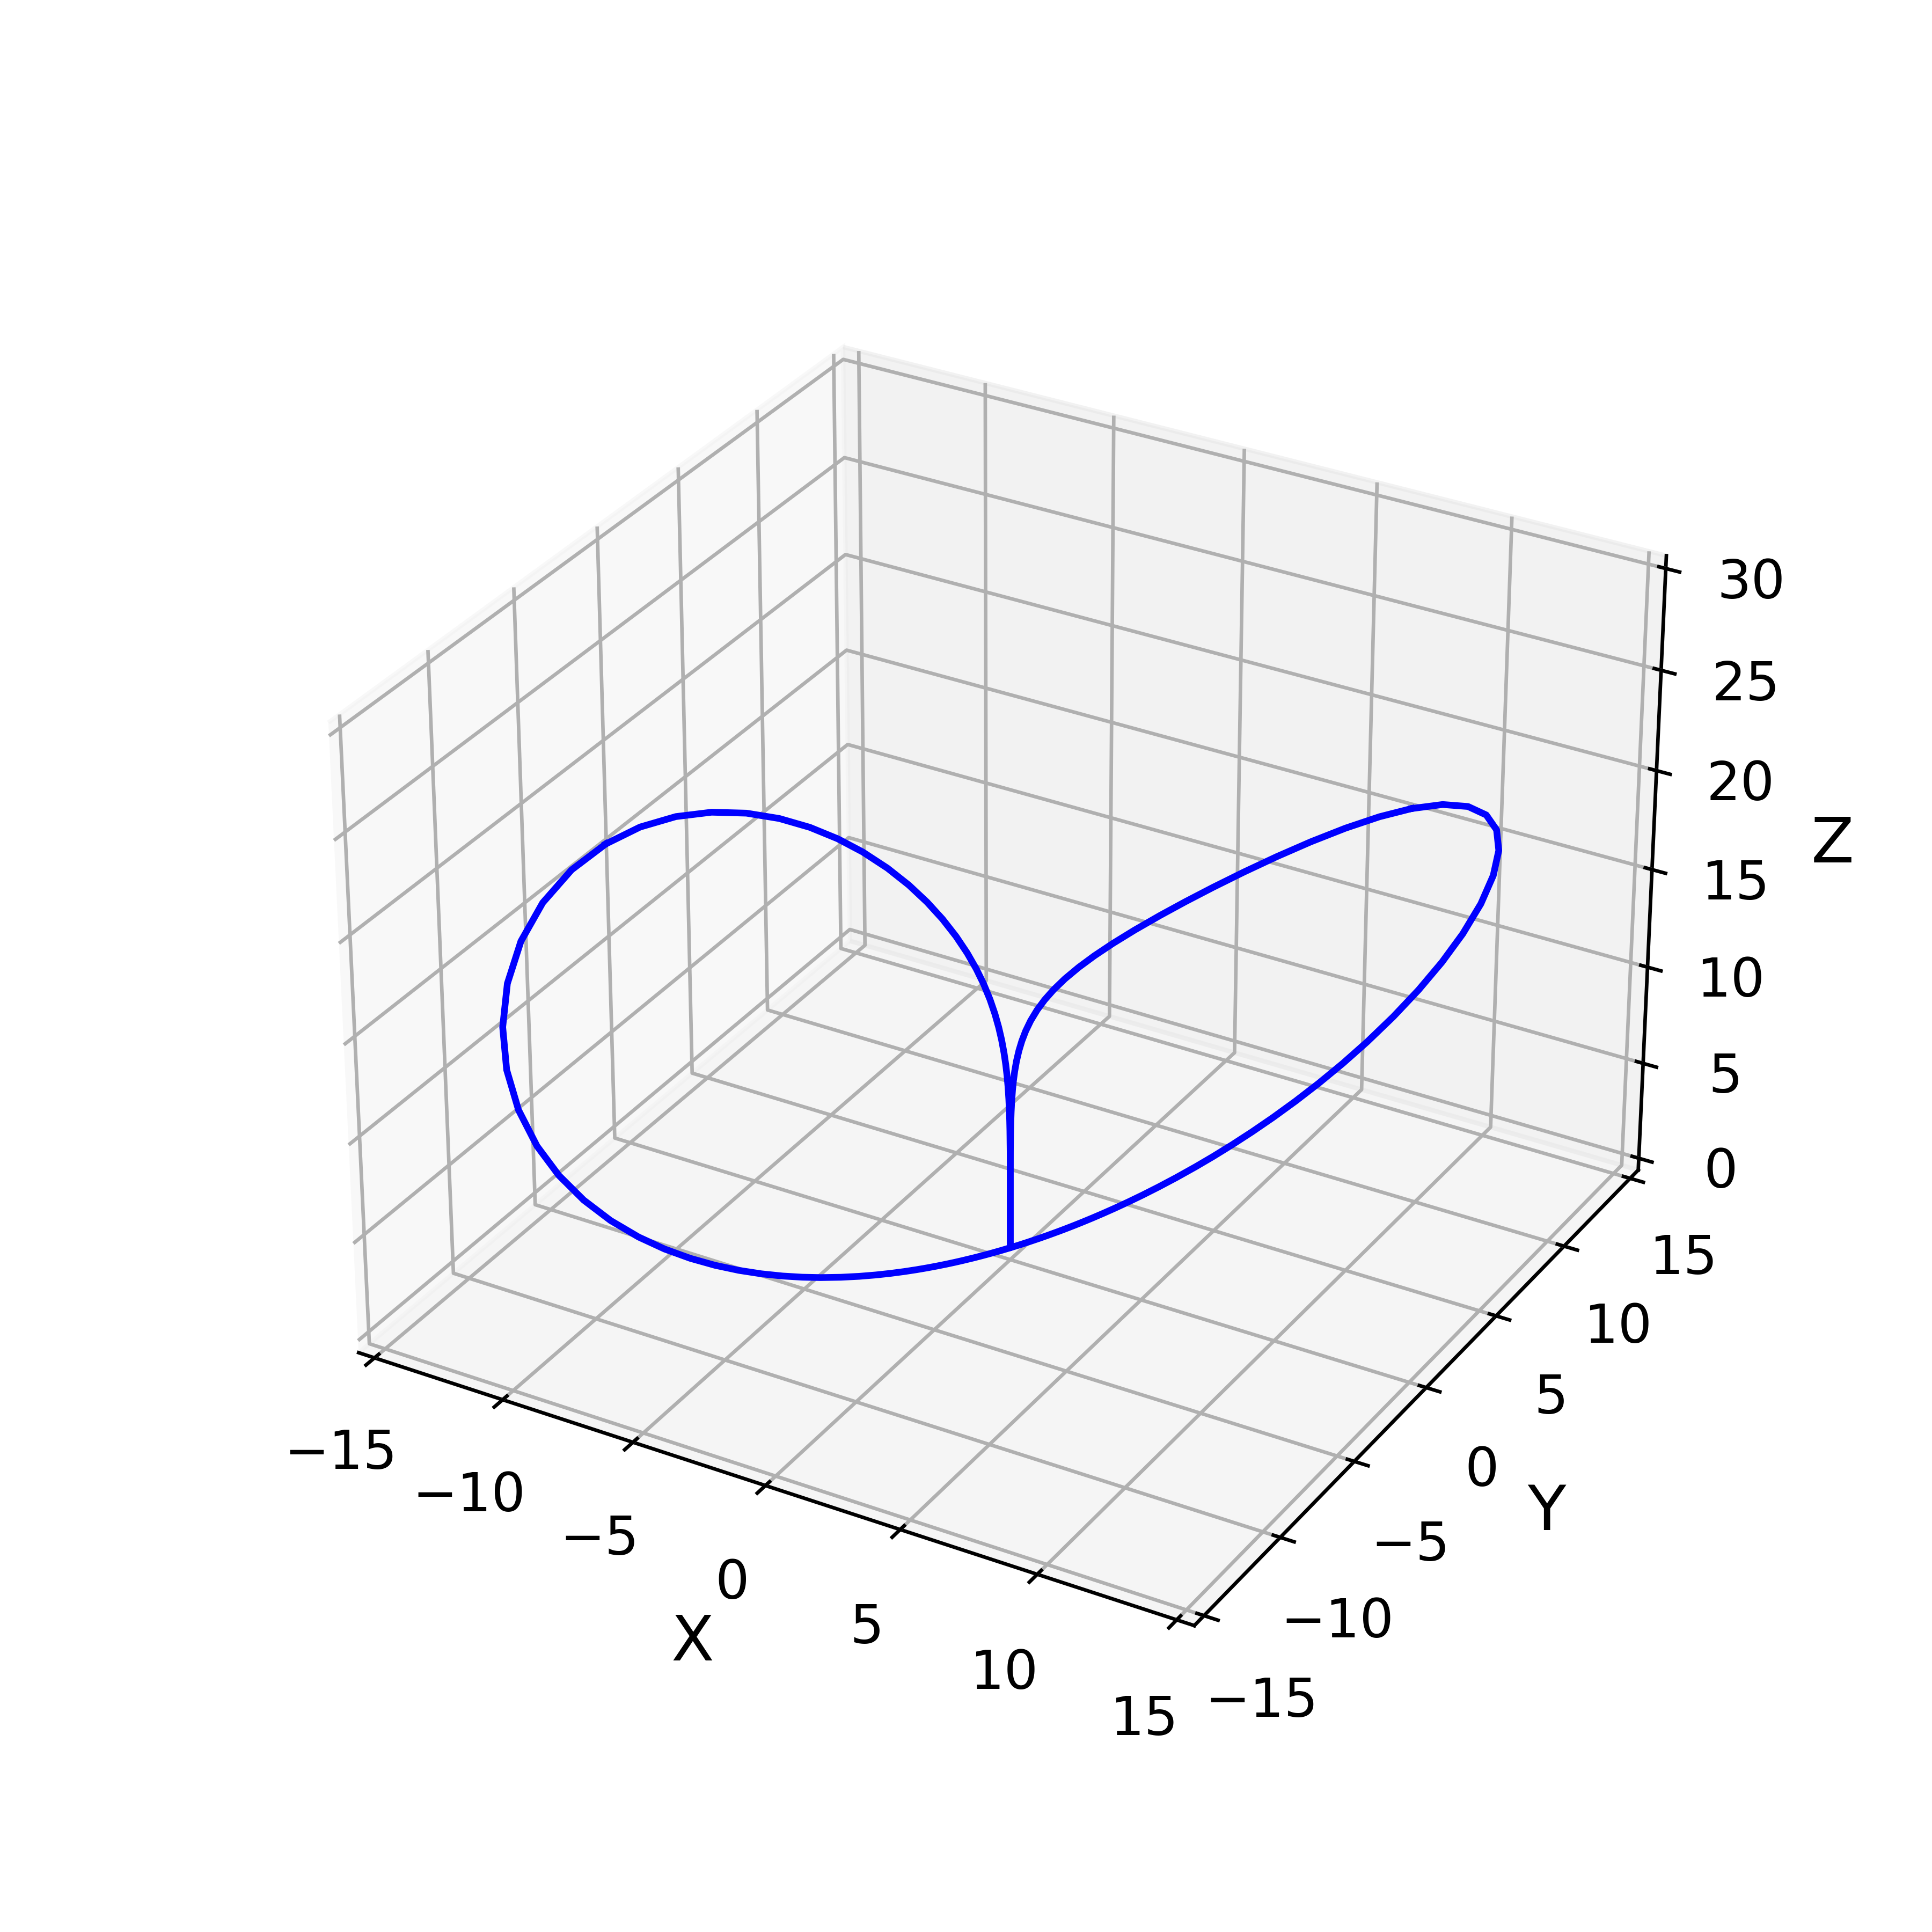
\includegraphics[width=\textwidth]{media/orbit_r_13.93.png}
		\caption{$r = 13.926$}
		\label{fig:sub2}
	\end{subfigure}
	
	\caption{Unstable periodic orbits in the Lorenz system for different values of $r$.}
	\label{fig:orbits}
\end{figure}

Figure \ref{fig:orbits} shows the unstable periodic orbits obtained using AUTO07p for different values of $r$. As $r$ decreases, the length of these orbits increases. At $r = 13.926$, the two periodic orbits merge at the origin, forming two homoclinic orbits. This indicates the occurrence of a homoclinic bifurcation. For $r < 13.926$, no periodic orbits are found.



\subsection{Chaos}

Lorenz found that for \( r > 24.74 \), trajectories do not settle to a fixed point or a periodic orbit but instead evolve on a complex set with a folded, butterfly-like structure - now known as the \textit{strange attractor}. Although this attractor resides in three-dimensional space, its dynamics are effectively constrained to a lower-dimensional manifold due to strong dissipation in the system. Figure~\ref{fig:chaos} shows the strange attractor and the corresponding time series for \( r = 28 \). The attractor exhibits two lobes, with the trajectory spiraling around one lobe before unpredictably switching to the other. This is reflected in the time series of \( X \) and \( Y \), which alternate between positive and negative values in an apparently random fashion. In the context of Rayleigh-Bénard convection, this implies that the fluid’s circulation repeatedly reverses direction - the strength and sense of the convective roll change irregularly over time. The system remains perpetually unsteady, and even though the equations are deterministic, the evolution is unpredictable in the long run. The strange attractor is observed to be completely dominant for r above 24.74 and almost any initial condition yields a trajectory that approaches the strange attractor. \\

\begin{figure}
\begin{subfigure}[b]{0.485\textwidth}
		\centering
		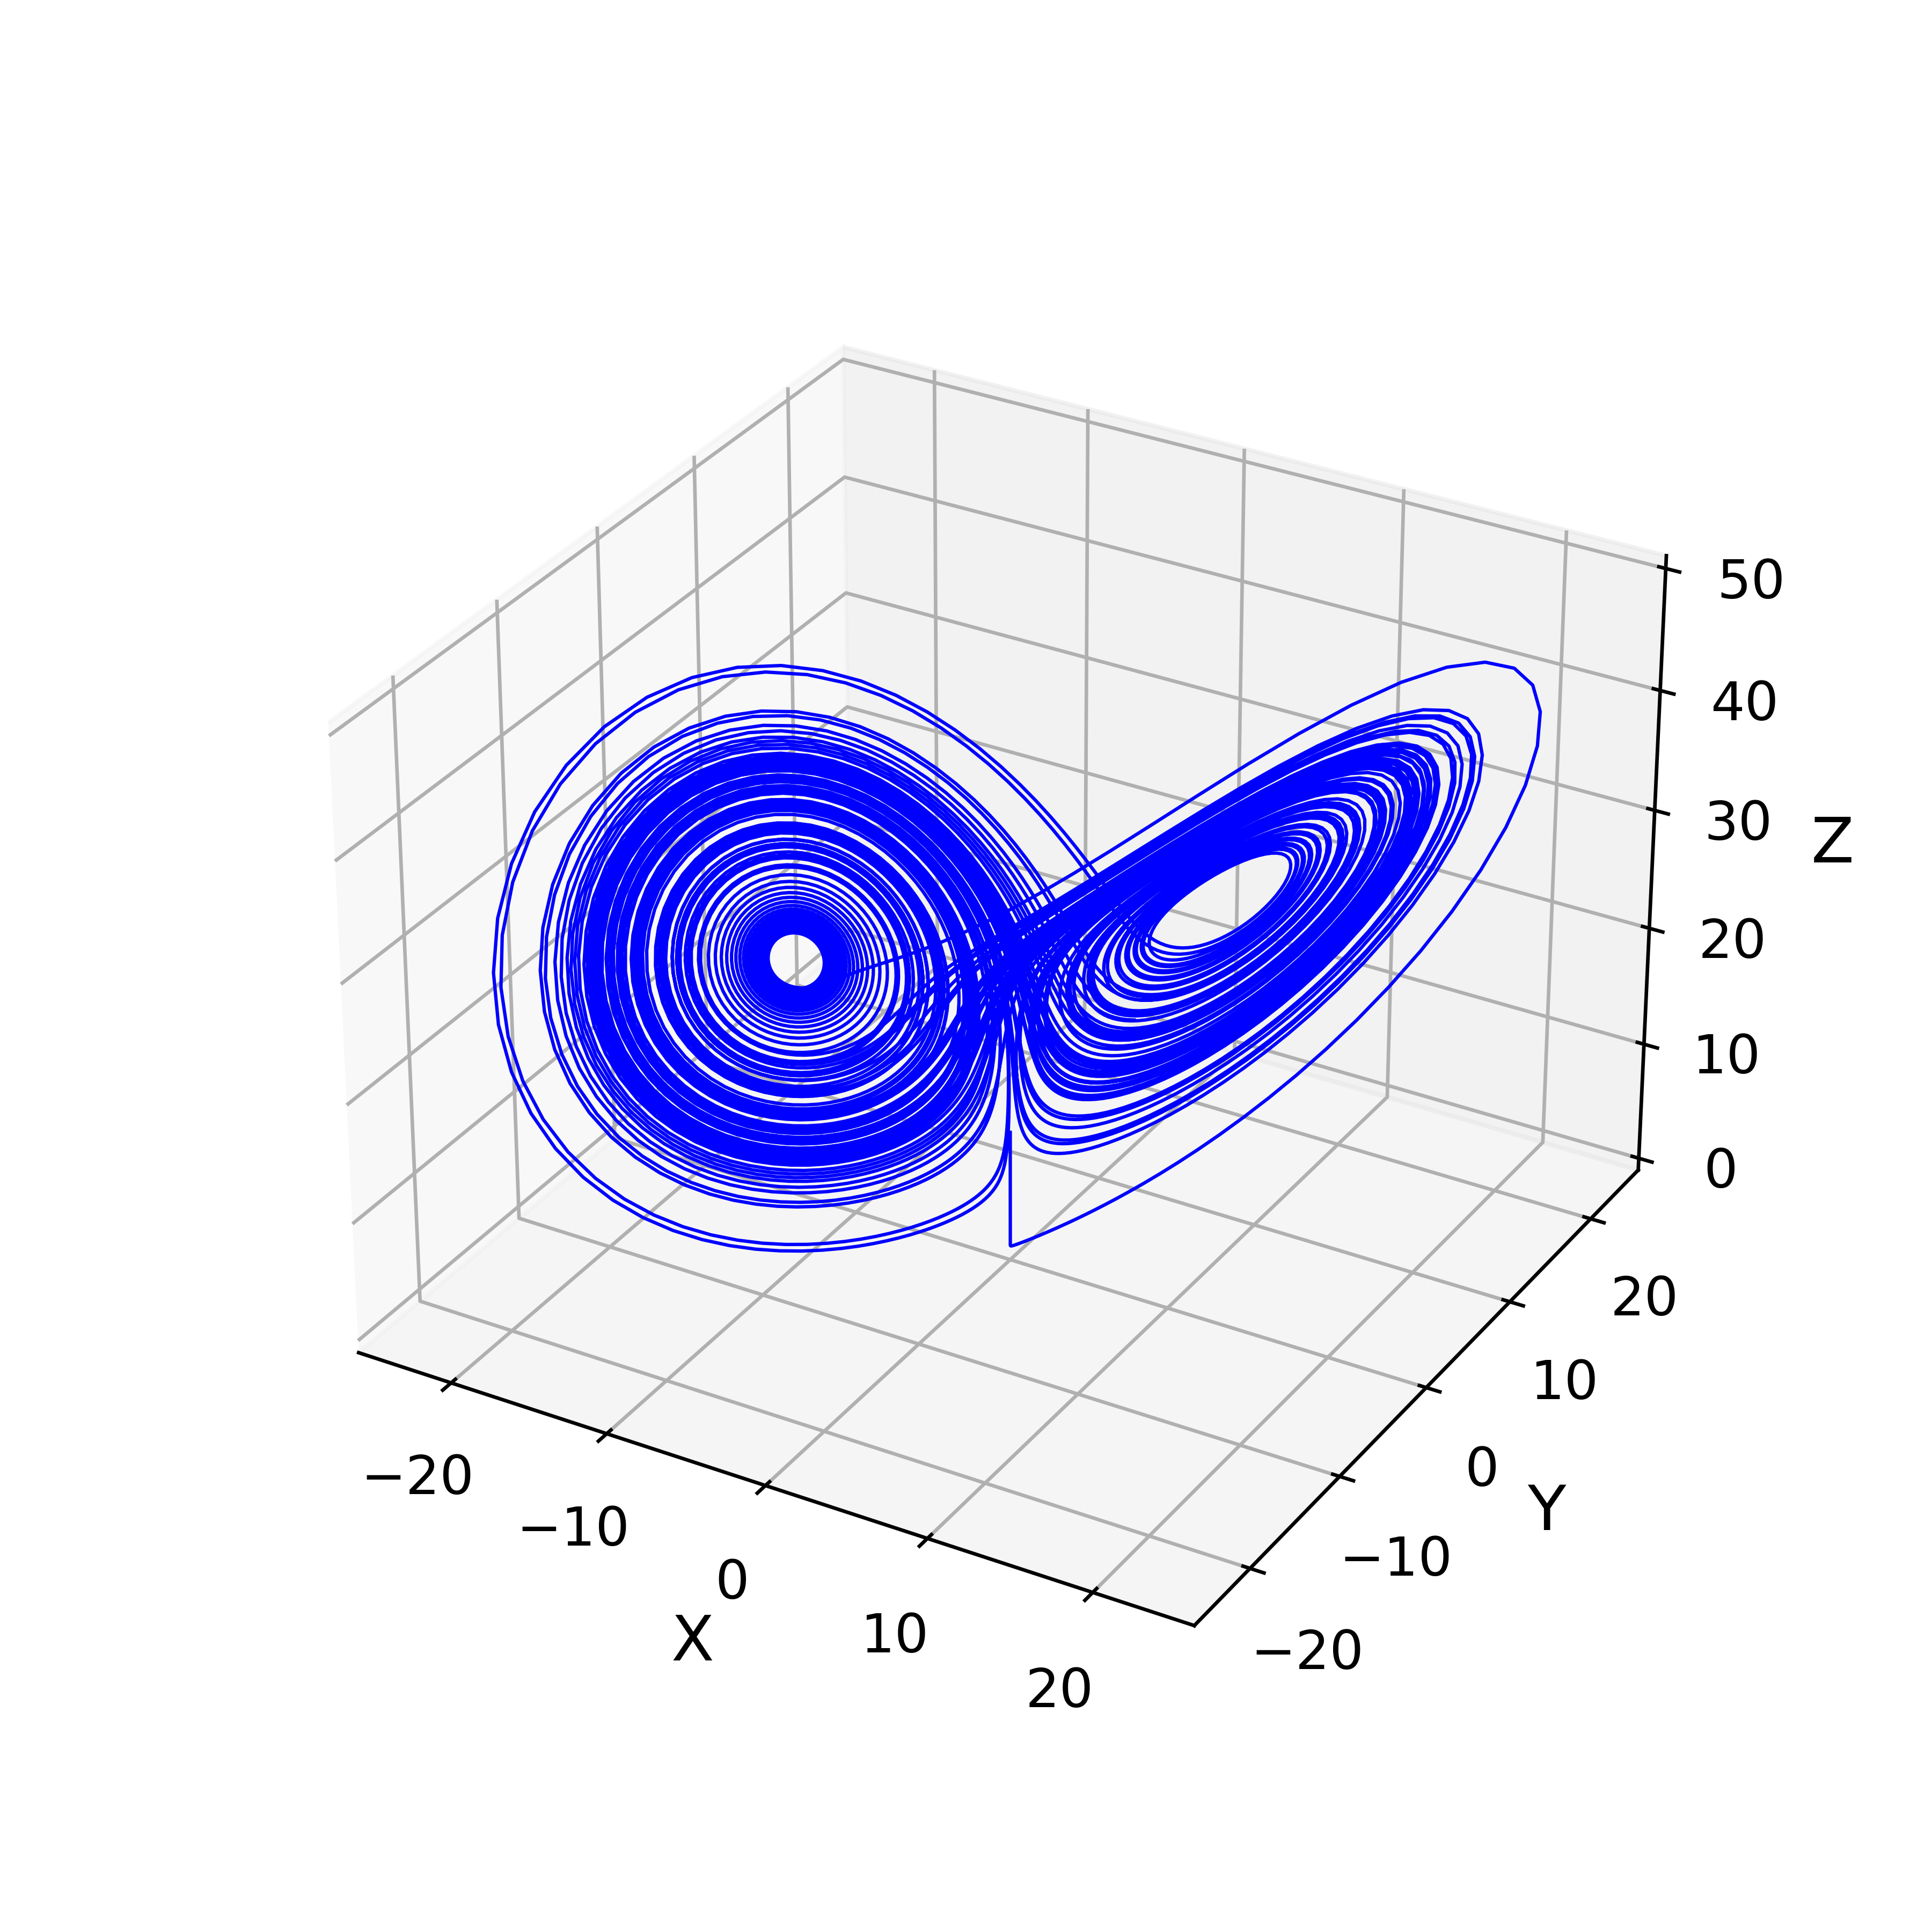
\includegraphics[width=\textwidth]{media/attractor_28.00.png}
		\caption{}
		\label{fig:sub1}
	\end{subfigure}
	\hfill
	\begin{subfigure}[b]{0.505\textwidth}
		\centering
		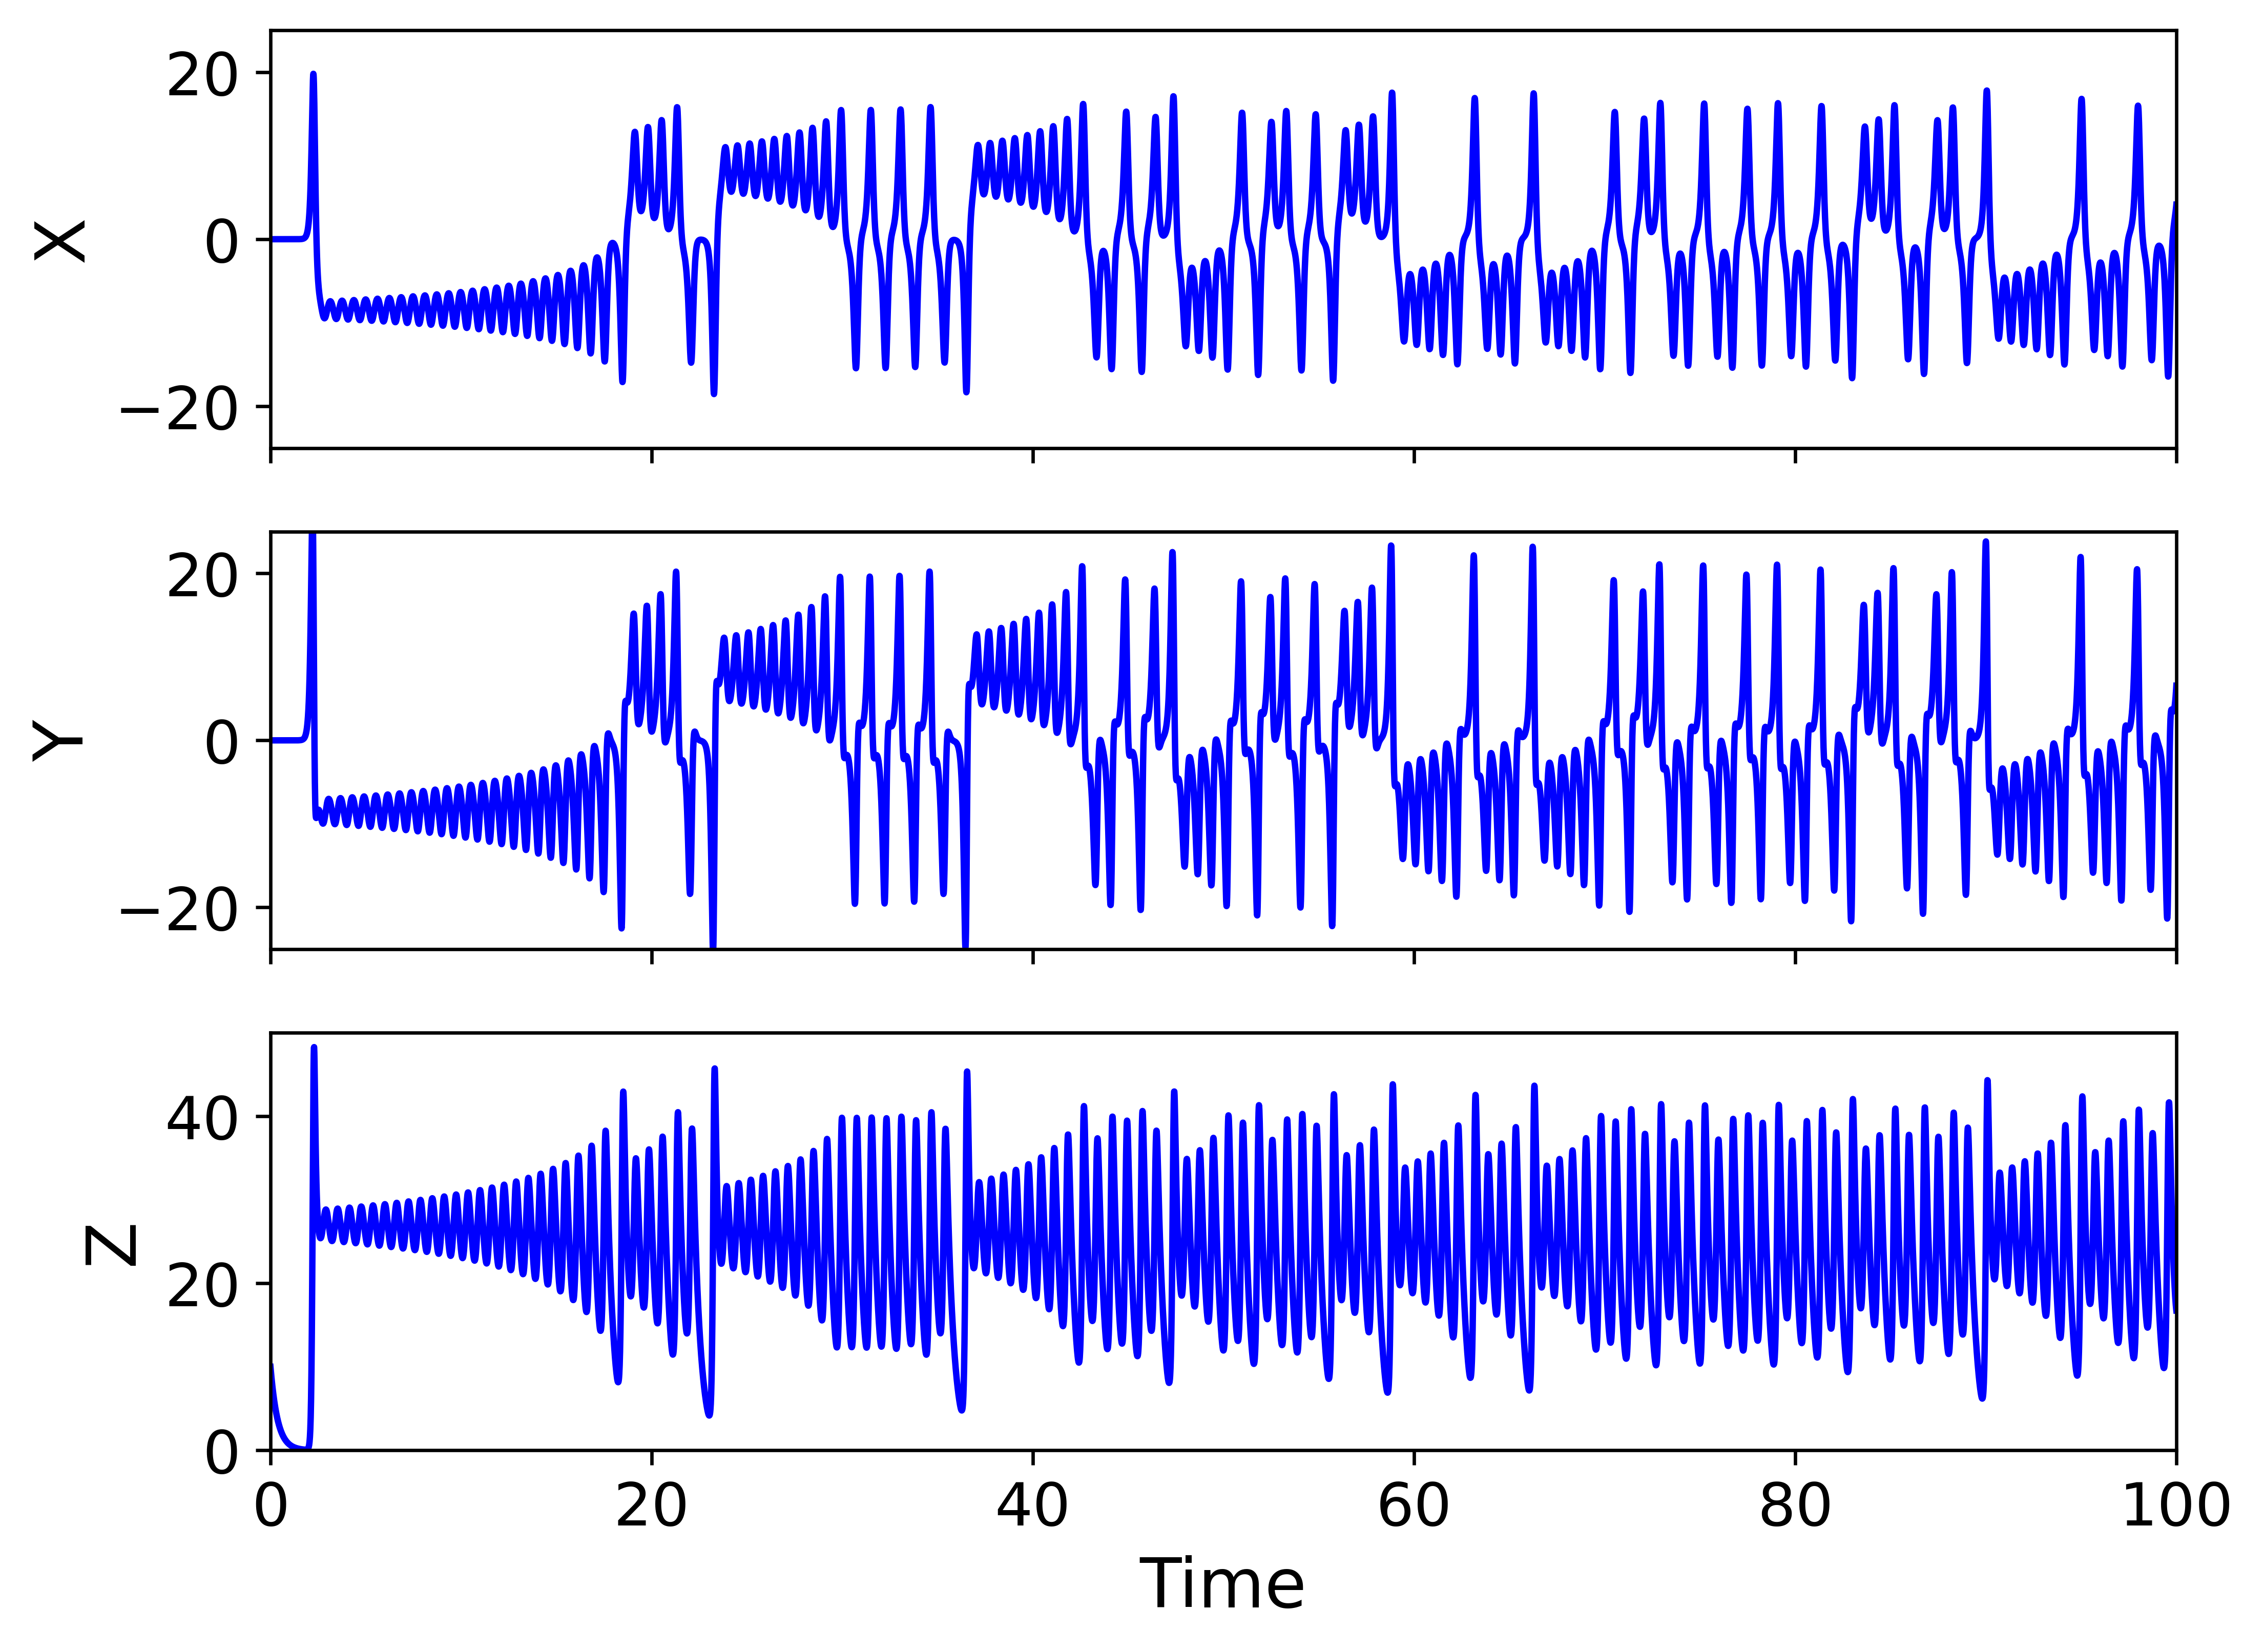
\includegraphics[width=\textwidth]{media/time_series_28.00.png}
		\caption{}
		\label{fig:sub2}
	\end{subfigure}
	
	\caption{Lorenz strange attractor and corresponding time series for \( r = 28 \).}
	\label{fig:chaos}
\end{figure}

An important characteristic of chaotic systems is their sensitive dependence on initial conditions. In the Lorenz system, even infinitesimally close initial states can lead to vastly different trajectories over time. This behavior is illustrated in Figure~\ref{fig:sensitivity}, where we track the evolution of two trajectories that start from nearly identical initial conditions. Initially, the trajectories remain close, but after some time, they diverge rapidly. The figure also includes a plot of the separation between the trajectories as a function of time. This separation increases exponentially at first but eventually saturates, since the dynamics are confined to a bounded region - the strange attractor - and the trajectories cannot drift arbitrarily far apart.\\

This exponential divergence is quantitatively captured by the largest Lyapunov exponent $\lambda_L$, which measures the average rate of separation of nearby trajectories:

\begin{equation}
	\delta(t) \sim \delta_0 \, e^{\lambda_L t}
\end{equation}
where $\delta(t)$ is the separation between trajectories at time $t$ and $\delta_0$ is the initial separation. A positive value of $\lambda_L$ indicates chaos. From our numerical simulation, we estimate $\lambda_L \approx 0.947$, which aligns well with values reported in the literature for the Lorenz system at $r = 28$, where $\lambda_L \approx 0.9$.

\begin{figure}[hbt!]
	\begin{subfigure}[b]{0.495\textwidth}
		\centering
		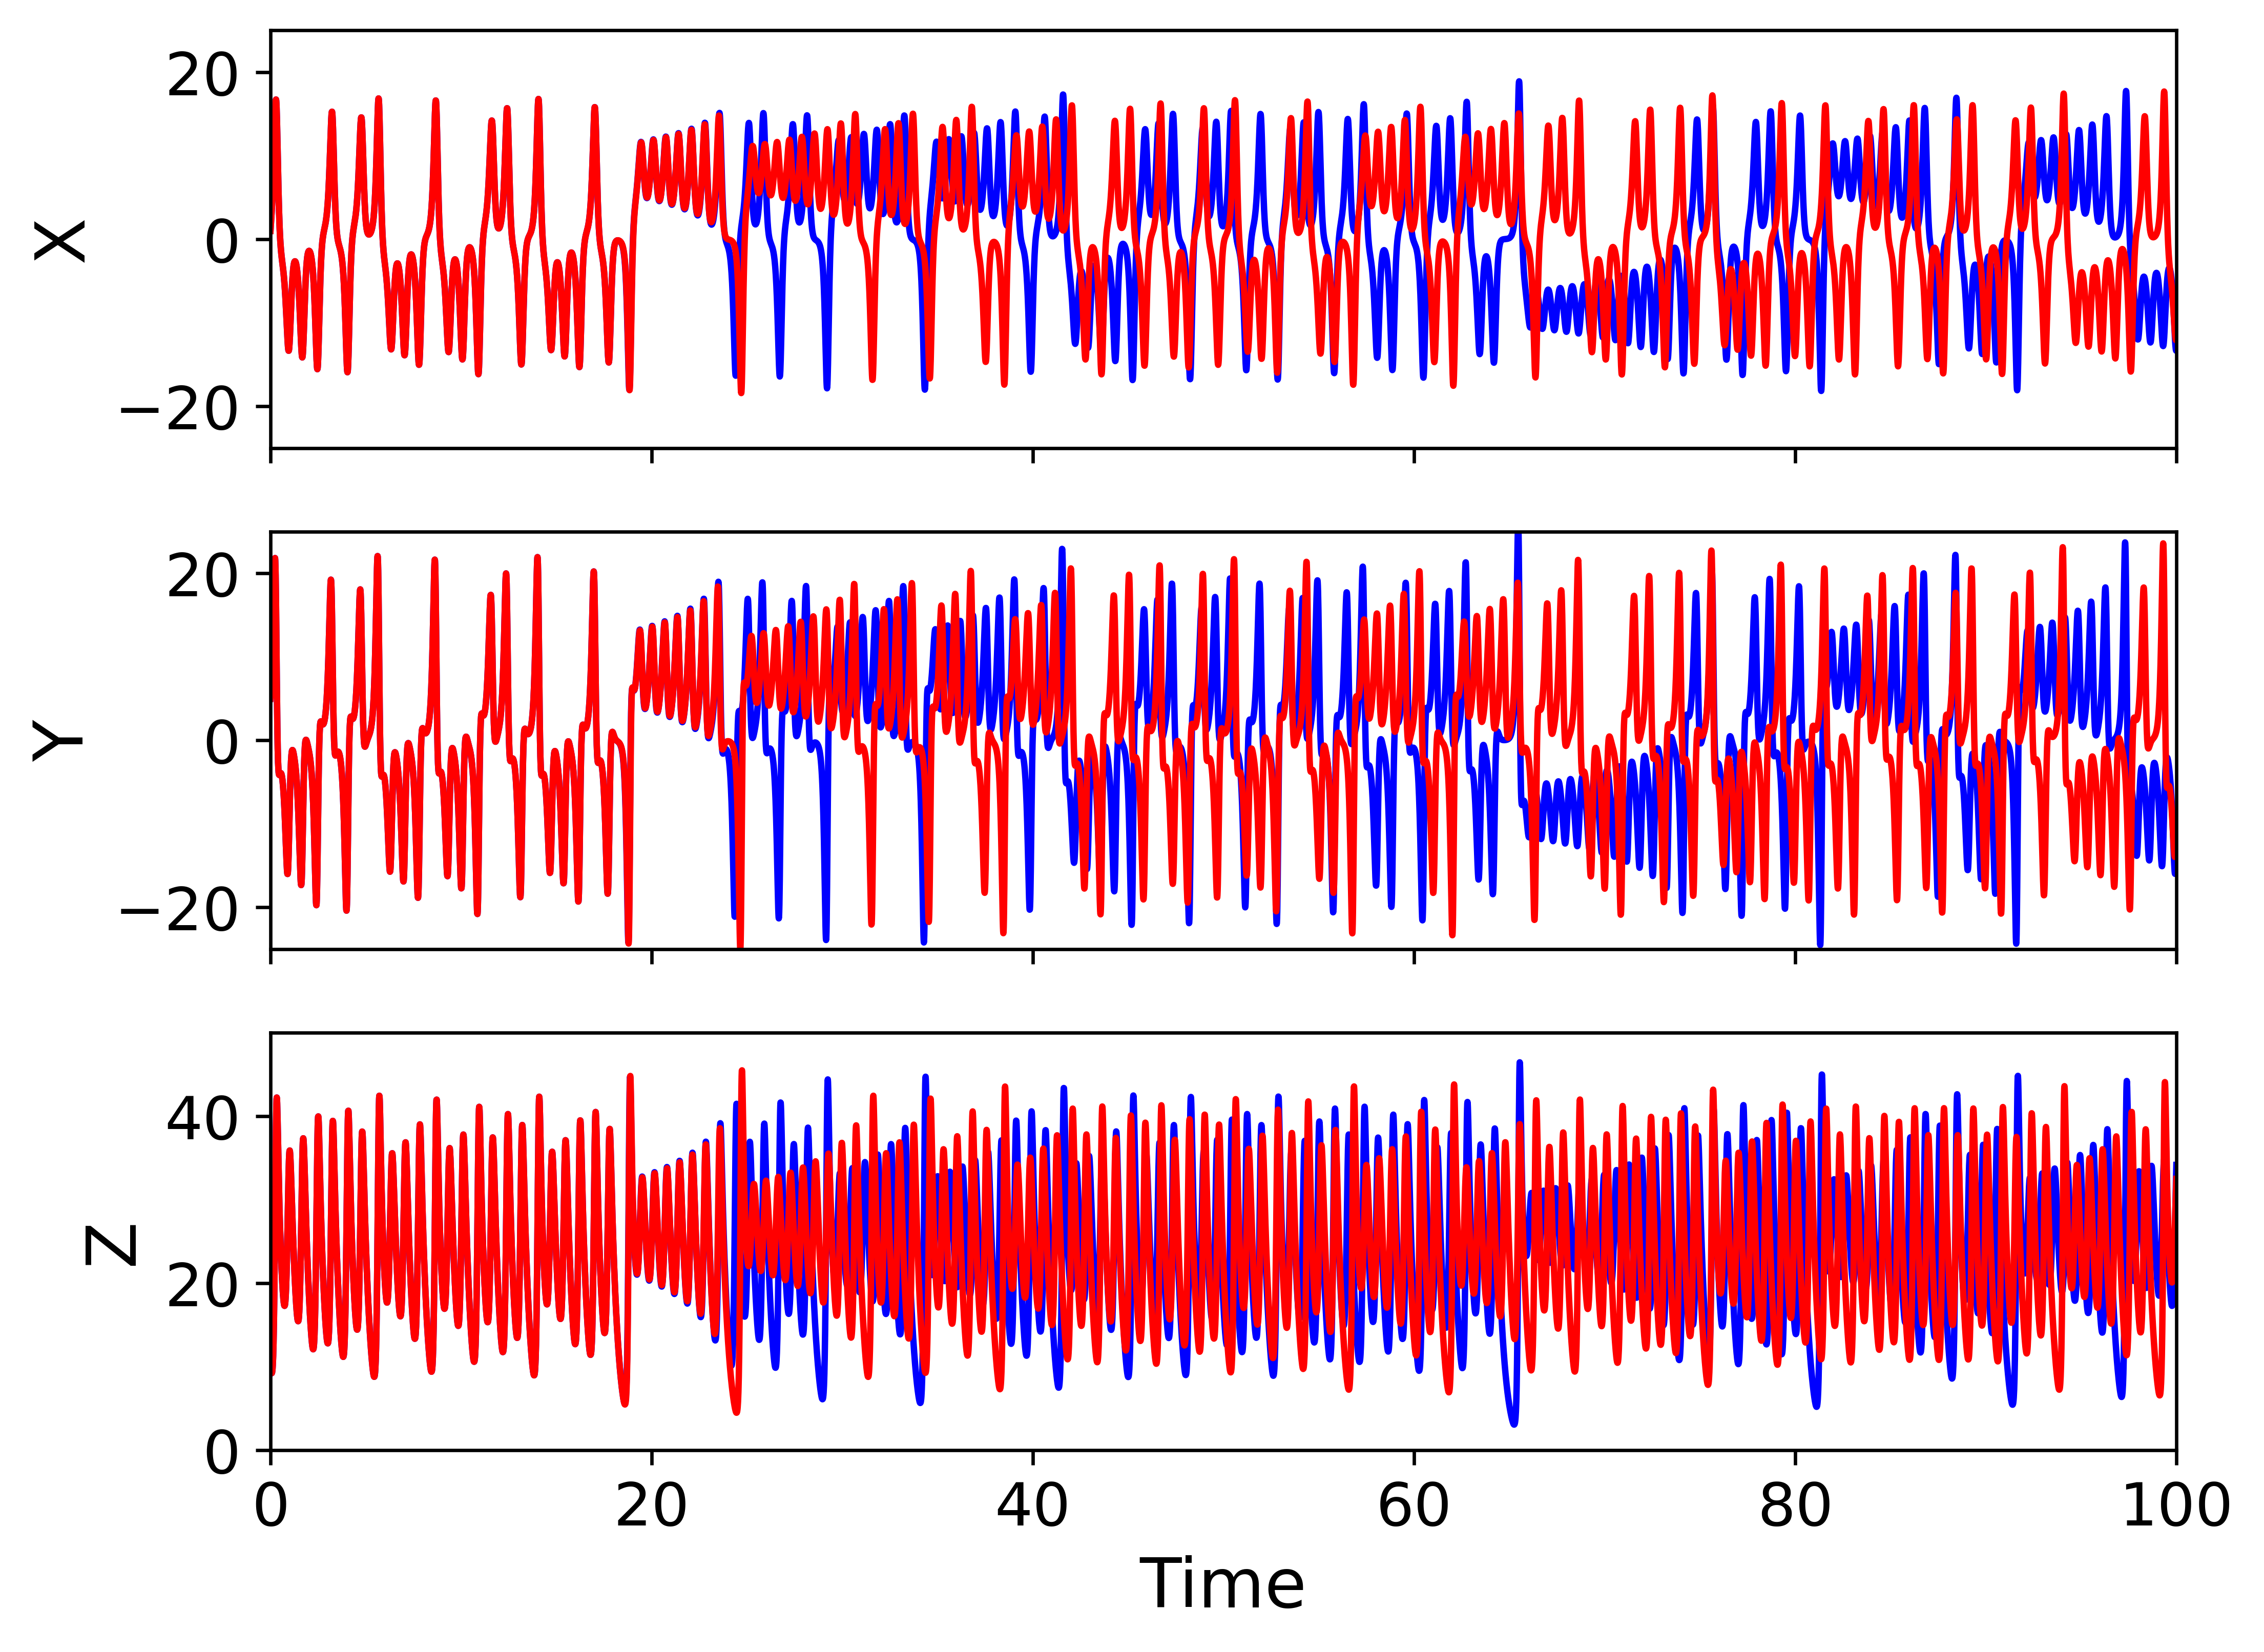
\includegraphics[width=\textwidth]{media/sensitivity_28.00.png}
		\caption{}
		\label{fig:sub1}
	\end{subfigure}
	\hfill
	\begin{subfigure}[b]{0.495\textwidth}
		\centering
		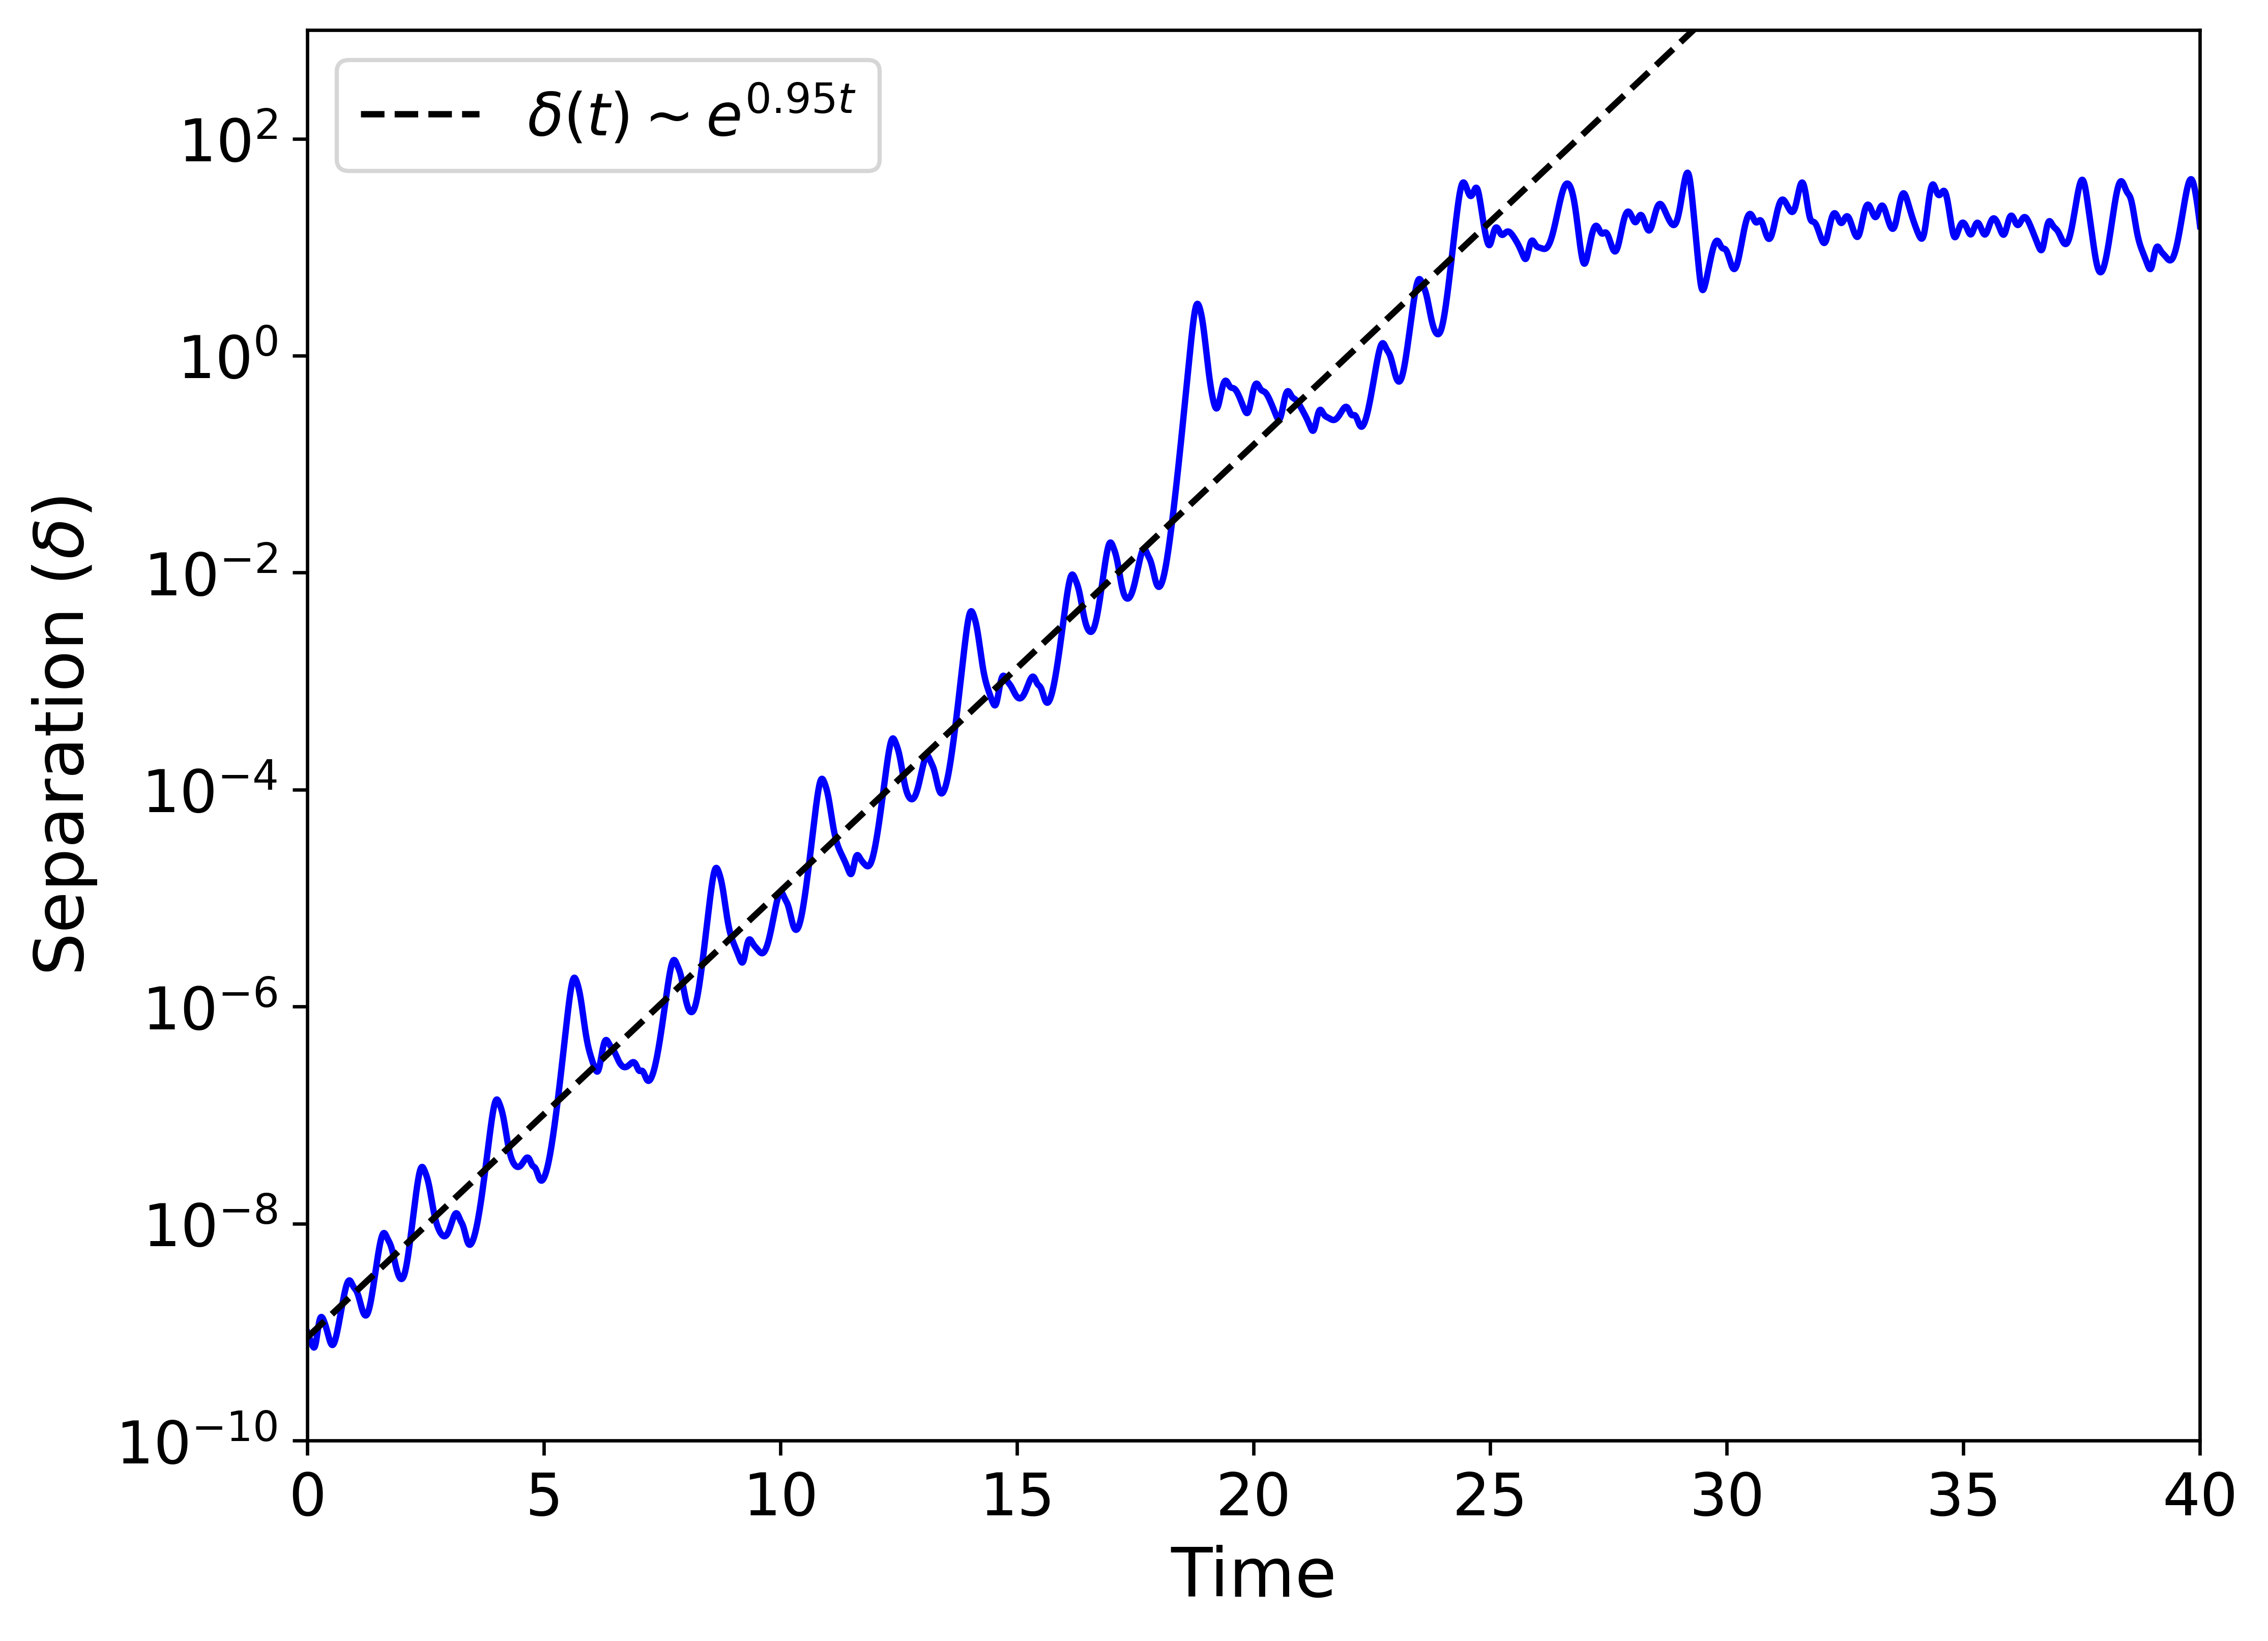
\includegraphics[width=\textwidth]{media/separation_28.00.png}
		\caption{}
		\label{fig:sub2}
	\end{subfigure}
	
	\caption{Sensitivity to initial conditions in the Lorenz system for \( r = 28 \).}
	\label{fig:sensitivity}
\end{figure}

\subsection{Metastable Chaos}
It has been shown by Yorke and Yorke~\cite{Yorke1979} that immediately after the homoclinic bifurcation at \( r = 13.926 \), there exists an ``exceptional'' set---a measure-zero set---of chaotic orbits that oscillate indefinitely. This chaotic set behaves dynamically like a saddle: most trajectories that start near it eventually diverge away. As a result, if an initial condition is randomly chosen from the neighborhood of this set, the probability that it oscillates forever without damping out is effectively zero. Although these truly chaotic orbits are not directly observable, their presence strongly influences nearby trajectories, especially for values of \( r \) approaching 24.74.\\

\begin{figure}[hbt!]
	\begin{subfigure}[b]{0.495\textwidth}
		\centering
		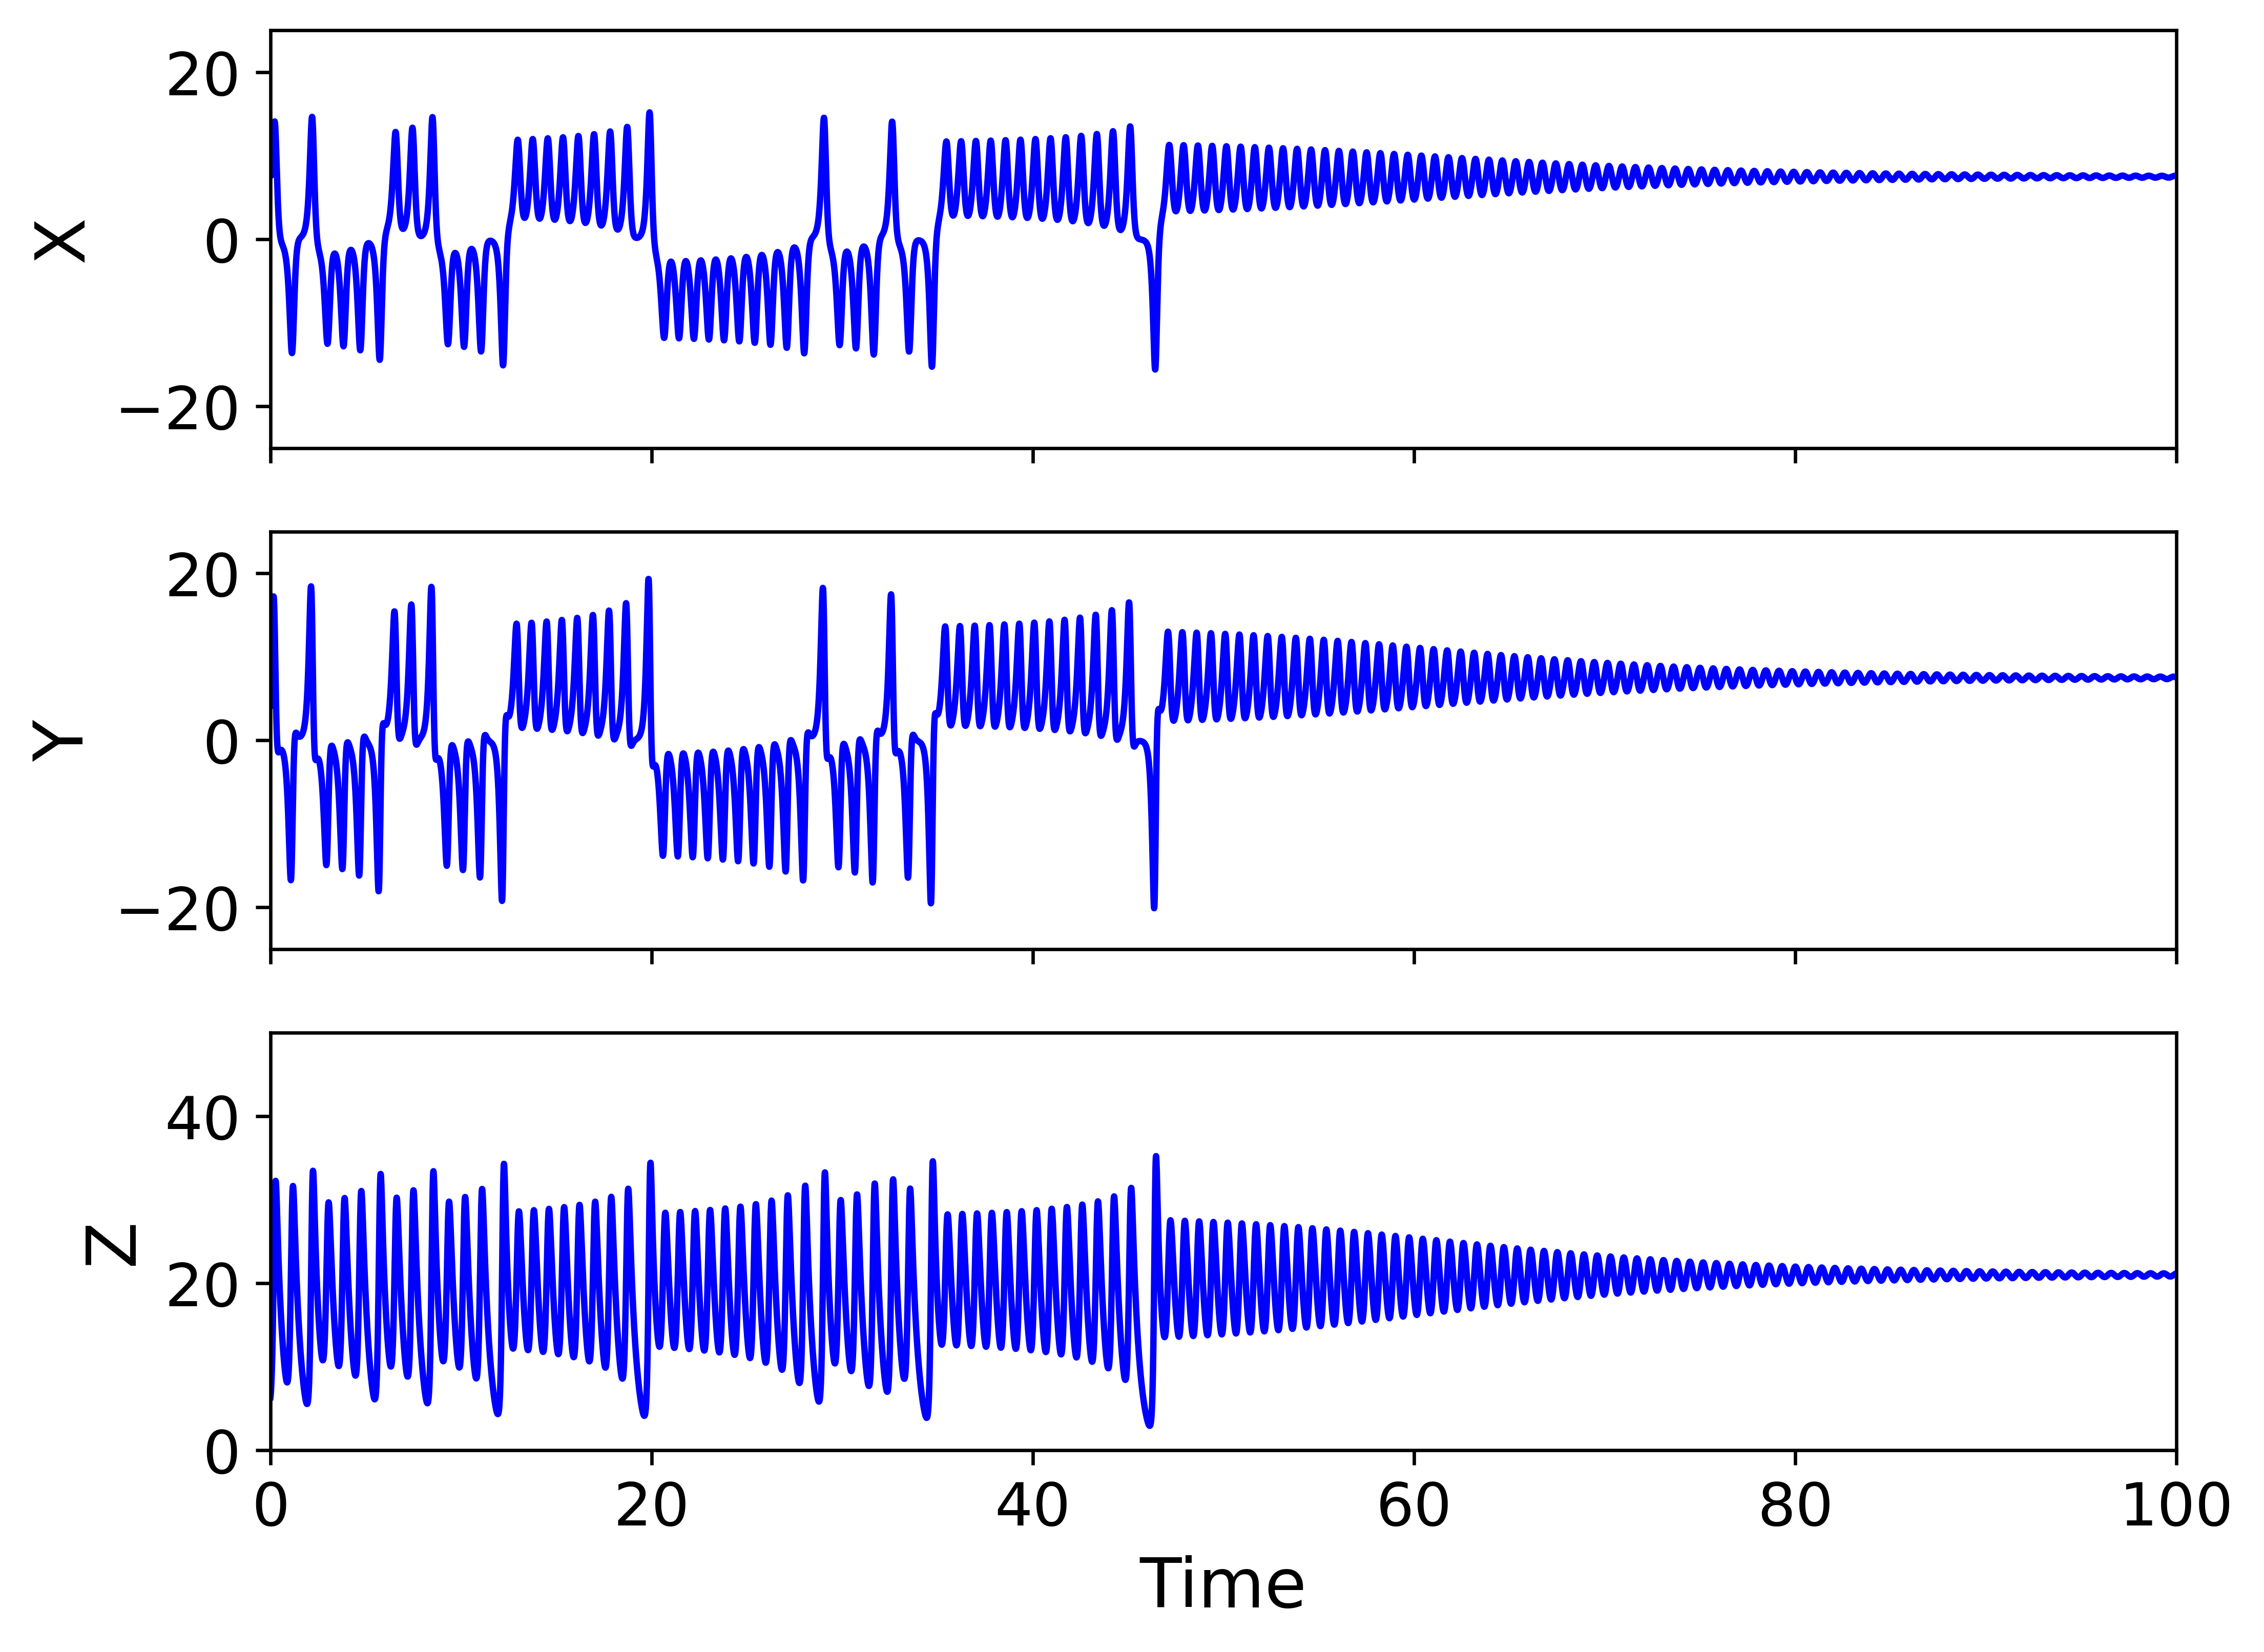
\includegraphics[width=\textwidth]{media/time_series_22.00.png}
		\caption{}
		\label{fig:sub1}
	\end{subfigure}
	\hfill
	\begin{subfigure}[b]{0.495\textwidth}
		\centering
		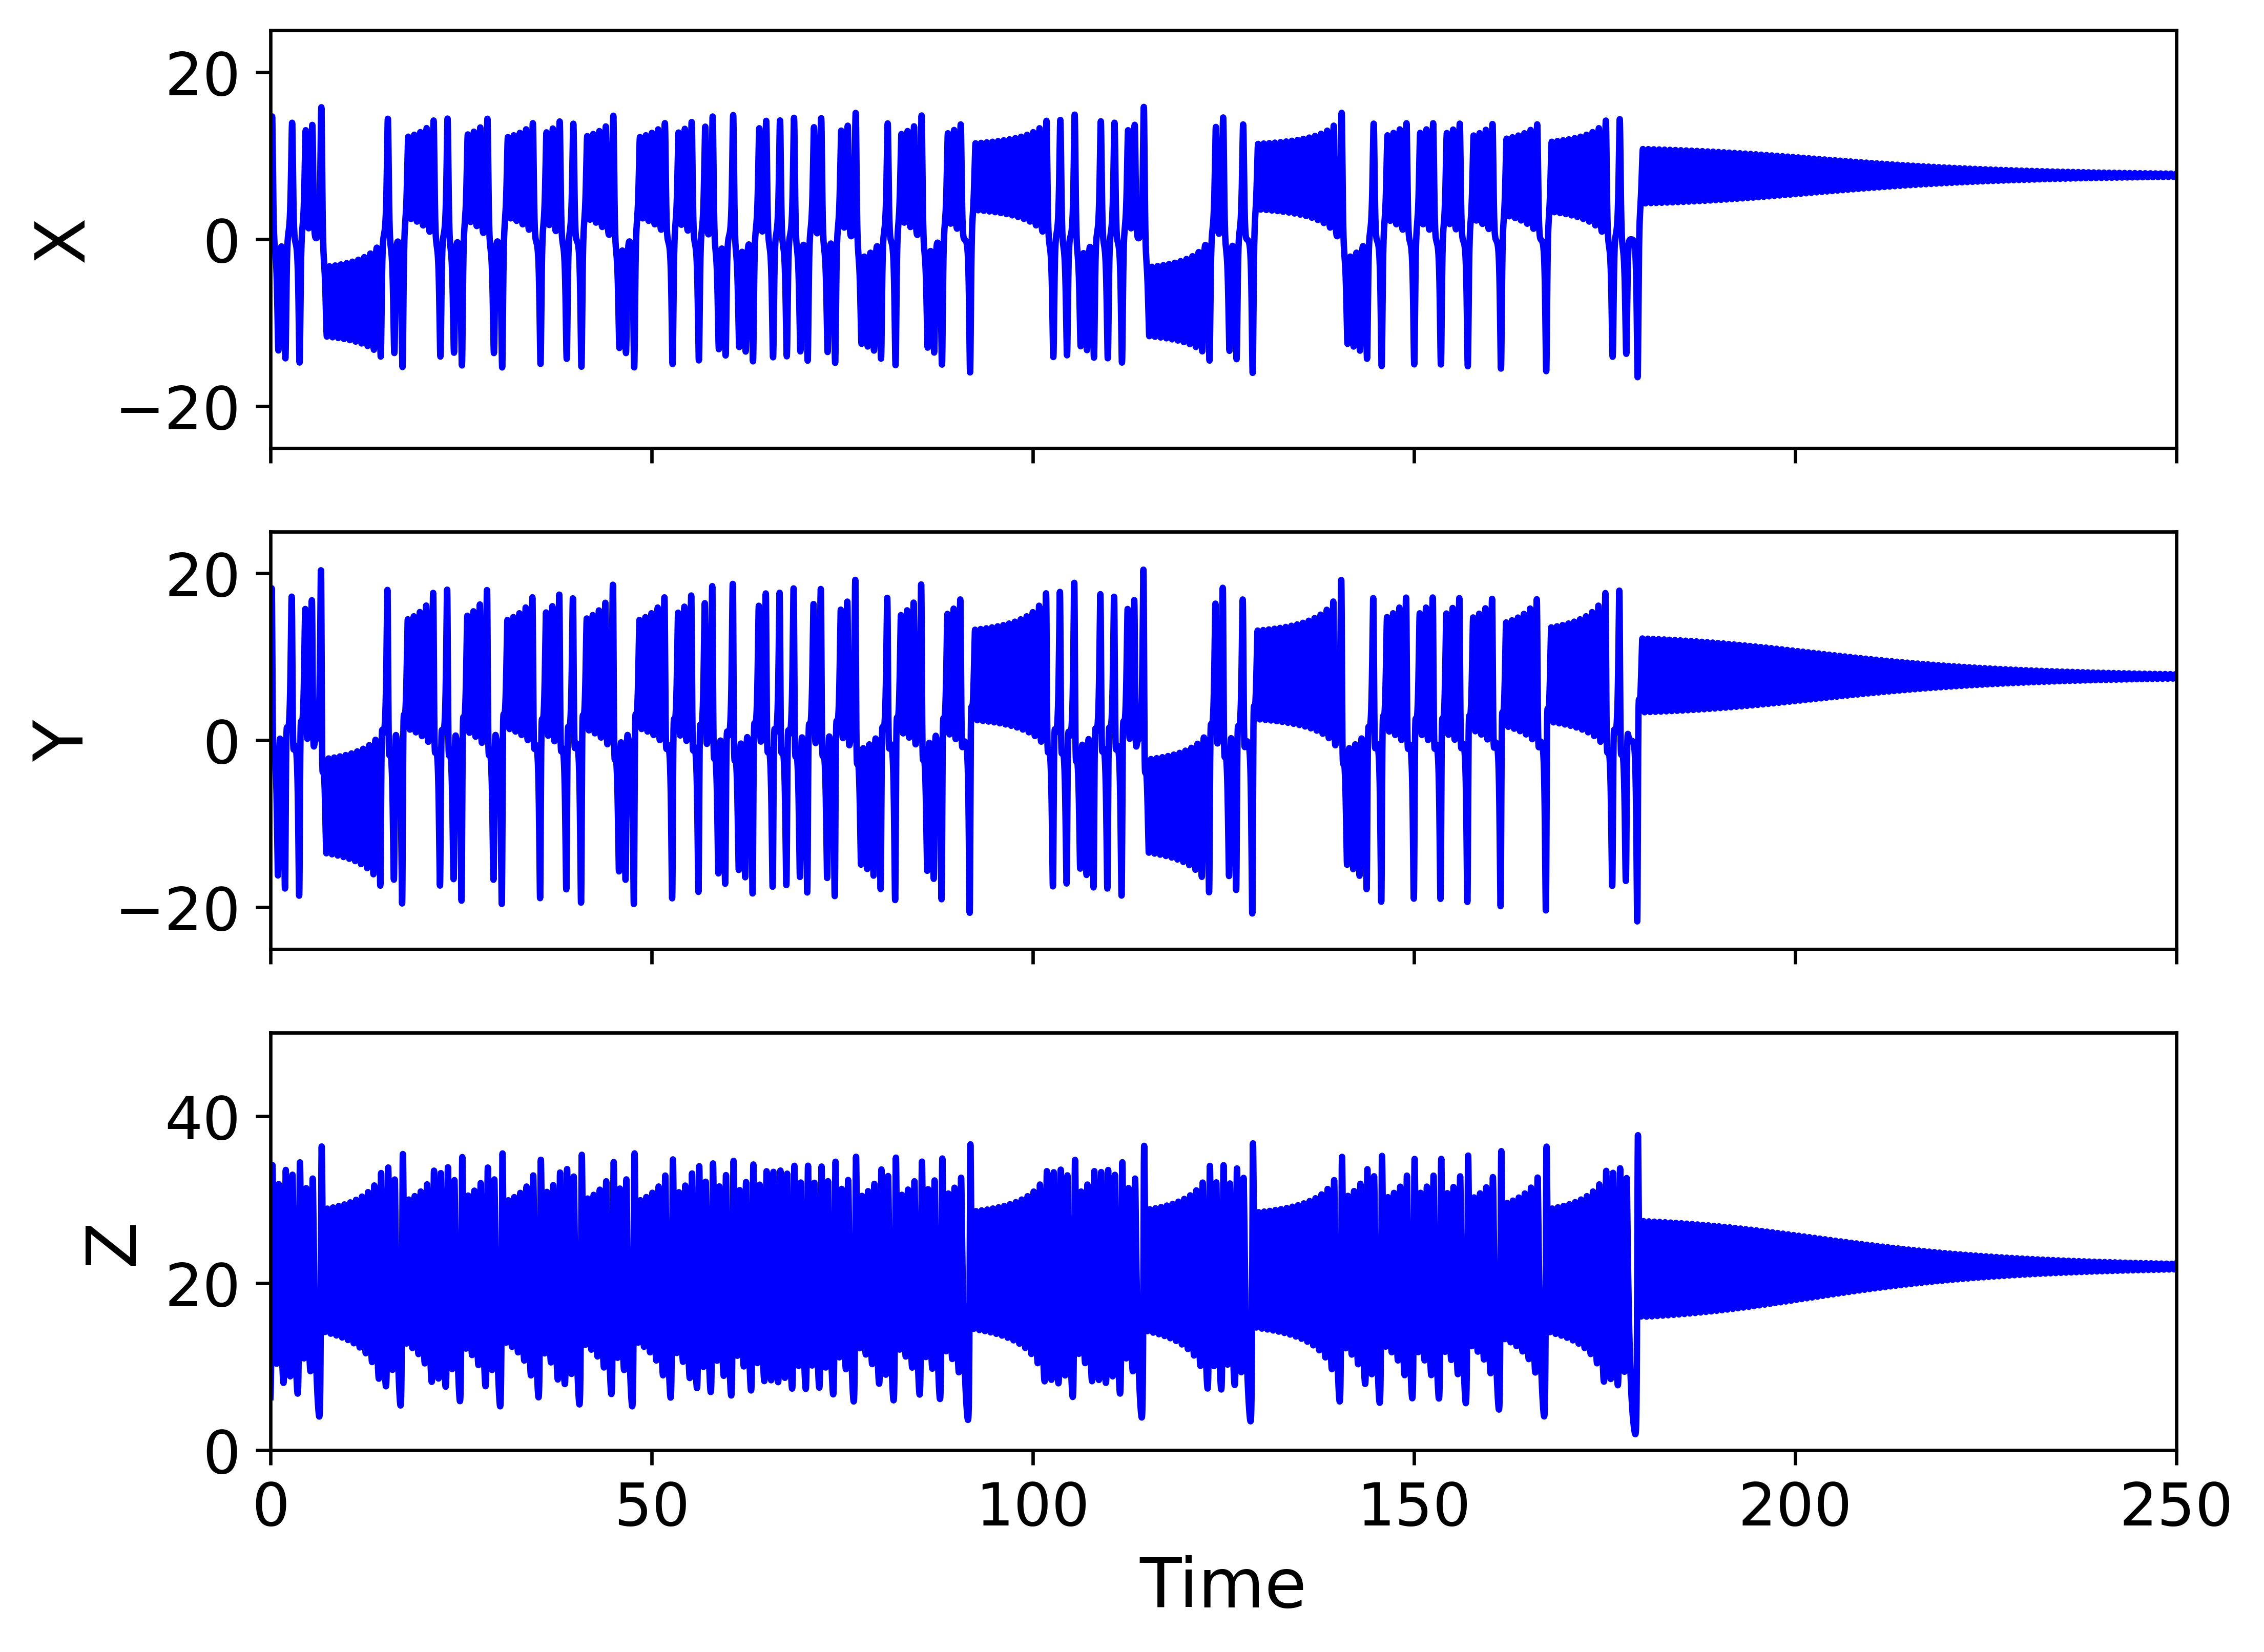
\includegraphics[width=\textwidth]{media/time_series_23.00.png}
		\caption{}
		\label{fig:sub2}
	\end{subfigure}
	
	\caption{Time series displaying metastable chaos for (a) $r = 22$ and (b) $r = 23$.}
	\label{fig:metastabletimeseries}
\end{figure}

This behavior can be seen in Figure~\ref{fig:metastabletimeseries}, which shows the time series of trajectories for two different values of \( r \) with the same initial condition. The trajectories initially exhibit chaotic oscillations, with random-like changes in sign, before eventually converging to one of the fixed points. This phenomenon, referred to as \emph{metastable chaos}, is characterized by an initial period of chaotic behavior followed by eventual stabilization. It is observed that the duration of the transient chaotic phase increases with \( r \): for the same initial conditions, the decay time is approximately 80 time units for \( r = 22 \) and around 240 time units for \( r = 23 \).\\

Figure~\ref{fig:metastableattractor} shows the trajectories in phase space along with the unstable limit cycles for two different initial conditions at $r=22$. The trajectories closely resemble the strange attractor structure seen at higher $r$, with the unstable limit cycles also appearing to lie on the same manifold. Initially, each trajectory is repelled by one of the limit cycles, oscillates around it, switches lobes, and then oscillates around the other limit cycle. This process repeats several times until the trajectory eventually lands inside one of the limit cycles, after which it asymptotically approaches one of the fixed points. It is thus the influence of the unstable limit cycles that gives rise to the observed transient chaotic behavior. Notably, although both trajectories start in the same region of phase space (the first quadrant), they end up settling into different fixed points due to the sensitivity induced by the transient chaos.\\

\begin{figure}[hbt!]
	\centering
	\begin{subfigure}[b]{0.495\textwidth}
		\centering
		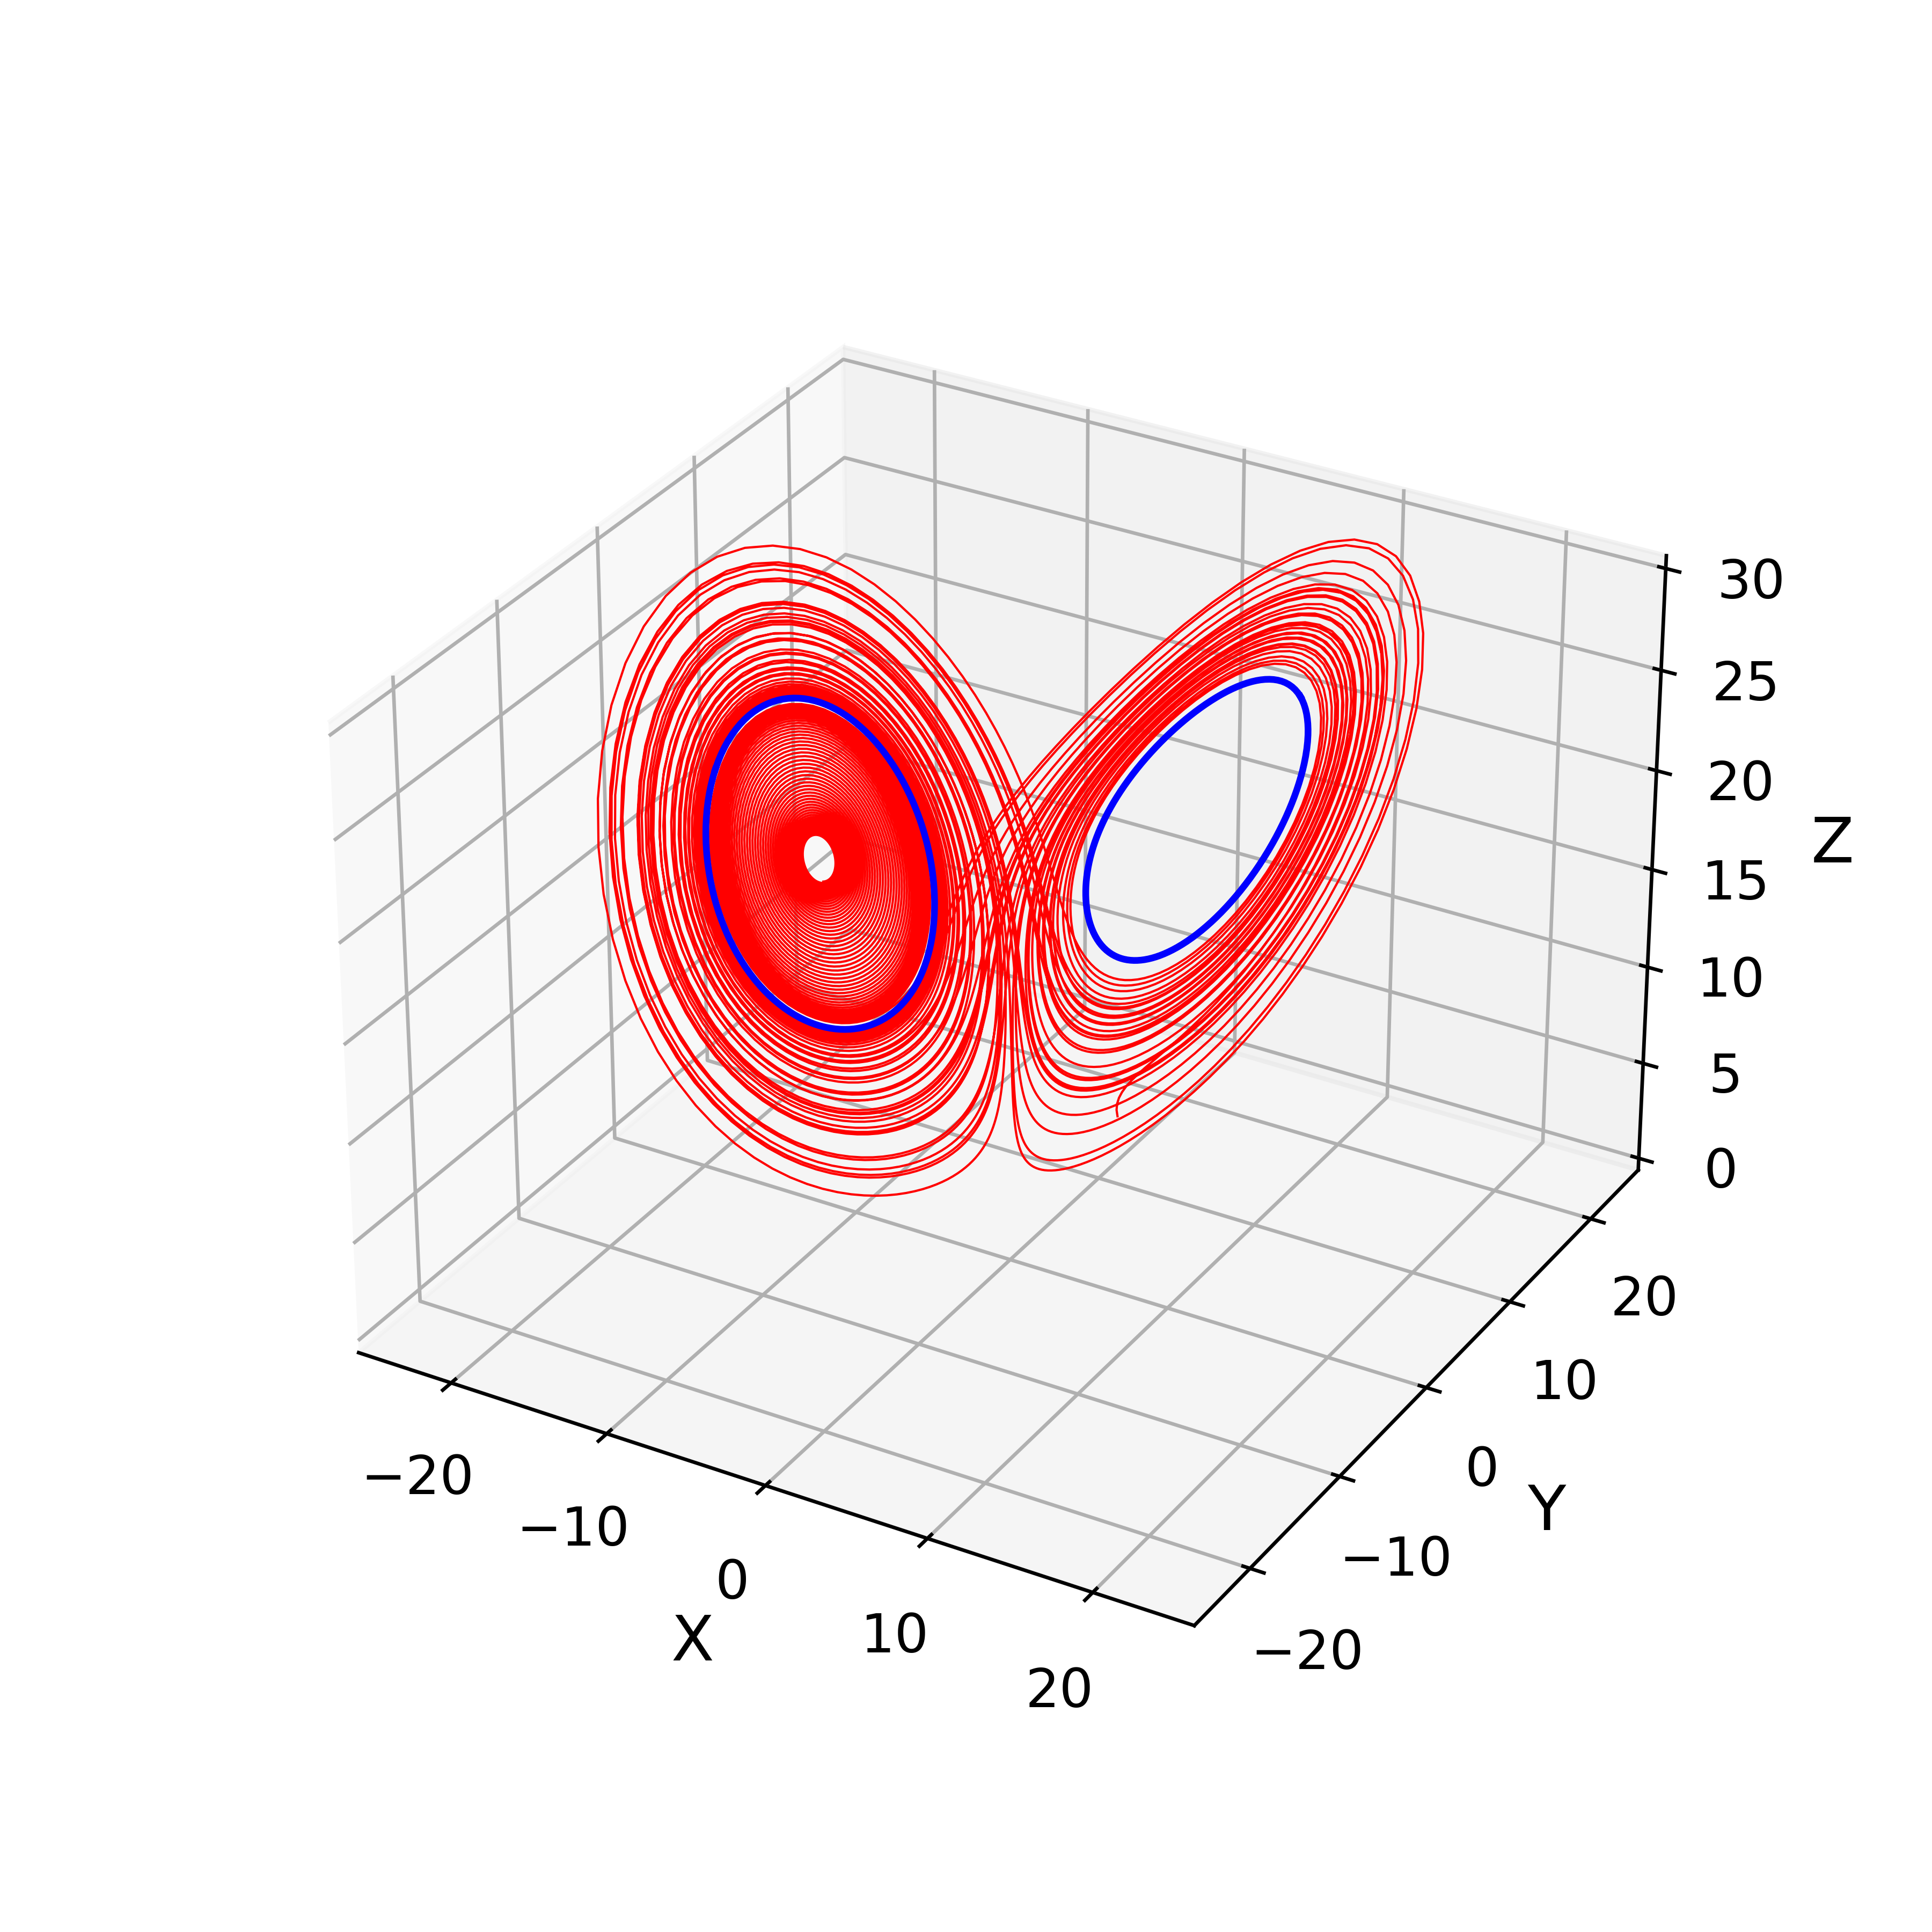
\includegraphics[width=\textwidth]{media/attractor_with_orbit_r_22.08_seed_2.png}
		\caption{}
		\label{fig:sub1}
	\end{subfigure}
	\hfill
	\begin{subfigure}[b]{0.495\textwidth}
		\centering
		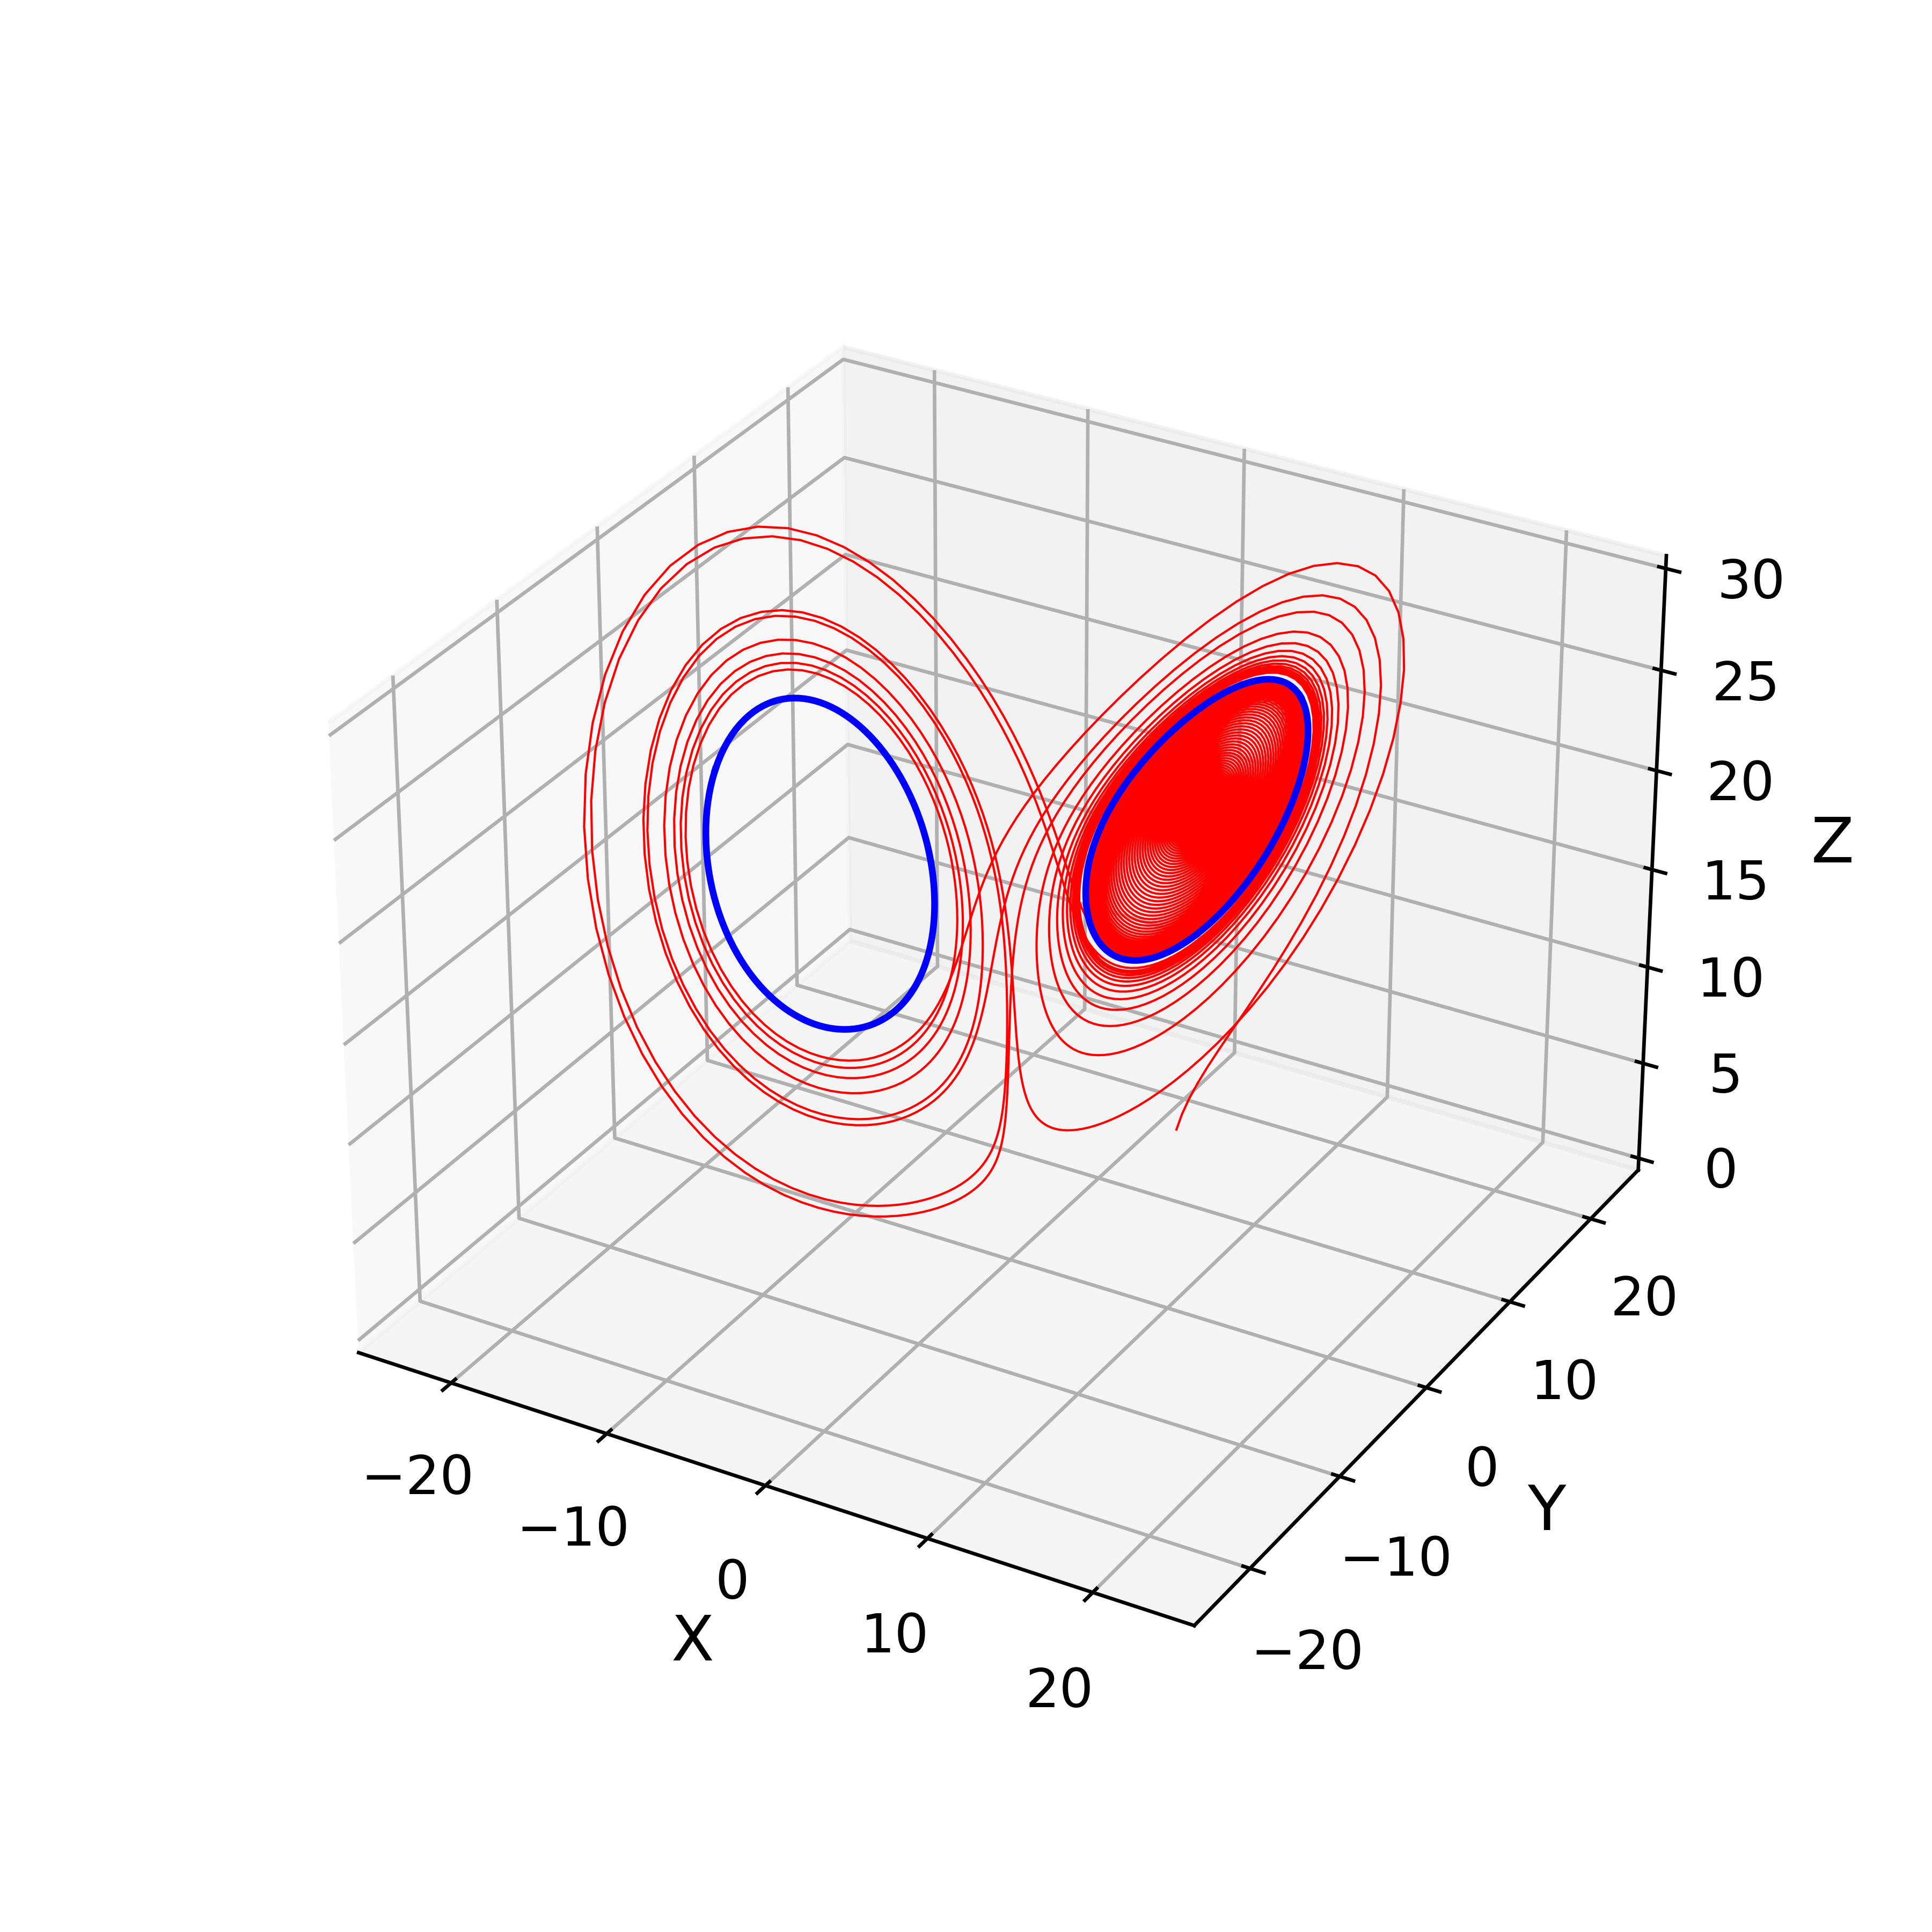
\includegraphics[width=\textwidth]{media/attractor_with_orbit_r_22.08_seed_100.png}
		\caption{}
		\label{fig:sub2}
	\end{subfigure}
	
	\caption{Evolution of the system trajectory (red) in phase space for two different initial conditions, shown alongside the unstable limit cycles (blue) for $r = 22$.}
	\label{fig:metastableattractor}
\end{figure}

As $r$ increases, the average decay time associated with metastable chaos also increases. Eventually, at $r=24.74$, the unstable limit cycles disappear in the Hopf bifurcation, and the system transitions to sustained chaotic behavior characterized by the strange attractor. Beyond this point, trajectories no longer settle into fixed points but continue to exhibit persistent chaotic oscillations.

\section{The Extended Lorenz System}
The Lorenz system modeled using only the sinusoidal horizontal mode, introduces a limitation in that the convection rolls have a fixed geometry. For example, the boundary at $x=0$ represents the division between two neighboring rolls, with only the speed and direction of circulation of the rolls changing over time. This results in a loss of the translational symmetry inherent in the original problem, which assumes an infinite extent in the x-direction. The truncation scheme used in this approach effectively constrains the system to a fixed, spatially periodic pattern, which does not fully capture the true dynamics of the problem. To address this issue, Chen and Price \cite{chen2006} proposed a five-mode truncation scheme that preserves the translational symmetry, leading to an extended Lorenz system capable of more accurately representing the behavior of the fluid convection system.

\subsection{Modeling}
The governing equations \ref{ndstreamfunctioneqn}-\ref{ndtemperatureeqn} are invariant under translation in the x-direction i.e. $(\psi(x,z,t),\theta(x,z,t))$ is a solution \textit{if and only if} $(\psi(x+\Delta x,z,t),\theta(x+\Delta x,z,t))$ is also a solution for any real $\Delta x$. We see that the mode $sin \, kx  \, sin \, \pi z$ always co-exits with the mode $cos \, kx  \, sin \, \pi z$ due to this symmetry property. In particular, 
\begin{equation}
	sin \, k\biggl(x + \frac{\pi}{2k}\biggr) \, cos \, \pi z = cos \, kx \, cos \, \pi z 
\end{equation}
\begin{equation}
	cos \, k\biggl(x + \frac{\pi}{2k}\biggr) \, cos \, \pi z = - sin \, kx \, cos \, \pi z 
\end{equation}

\noindent We thus modify the Lorenz truncation scheme to the form 
\begin{equation}
	\psi(x,z,t) = \hat{\psi_1}(t) \, \phi_{k,1}(x,z) + \hat{\psi_2}(t) \, \varphi_{k,1}(x,z)
	\label{extpsi}
\end{equation}
\begin{equation}
	\theta(x,z,t) = \hat{\theta_1}(t) \, \varphi_{k,1}(x,z) + \hat{\theta_2}(t) \, \phi_{k,1}(x,z) - \hat{\theta_3}(t) \, \vartheta_2 (z)
	\label{exttheta}
\end{equation}

\noindent where the functions $\phi$, $\varphi$ and $\vartheta$ are defined in \ref{initpsi}, \ref{inittheta} and \ref{lorenztheta} respectively.\\

\noindent Substituting \ref{extpsi} and \ref{exttheta} in \ref{ndstreamfunctioneqn}-\ref{ndtemperatureeqn} and neglecting the additional modes generated, we get the following:

\begin{equation}
	\frac{d \hat{\psi_1}}{dt} \, \phi_{k,1} + \frac{d \hat{\psi_2}}{dt} \, \varphi_{k,1} = Pr \biggl[ \frac{k}{\gamma^2} (\hat{\theta_1} \, \phi_{k,1} - \hat{\theta_2} \, \varphi_{k,1}) - \gamma^2 (\hat{\psi_1} \, \phi_{k,1} + \hat{\psi_2} \, \varphi_{k,1})\biggr]
	\label{extpsieqn}
\end{equation}
\begin{equation}
	\begin{split}
		\frac{d \hat{\theta_1}}{dt} \, \varphi_{k,1} + \frac{d \hat{\theta_2}}{dt} \, \phi_{k,1} - \frac{d \hat{\theta_3}}{dt} \, & \vartheta_2 
		=  - \frac{k \pi}{2} (\hat{\psi_1} \hat{\theta_1} - \hat{\psi_2} \hat{\theta_2}) \, \vartheta_2 - k \pi (\hat{\psi_1} \hat{\theta_3} \, \varphi_{k,1} - \hat{\psi_2} \hat{\theta_3} \, \phi_{k,1}) \\ 
		& + Ra \, k (\hat{\psi_1} \, \varphi_{k,1} - \hat{\psi_2} \, \phi_{k,1}) - \gamma^2 (\hat{\theta_1} \, \varphi_{k,1} + \hat{\theta_2} \, \phi_{k,1}) 
		 + 4 \pi^2 \hat{\theta_3} \, \vartheta_2
	\end{split}
	\label{extthetaeqn}
\end{equation}

\noindent Projecting \ref{extpsieqn} and \ref{extthetaeqn} onto the modes, we obtain:
\begin{equation}
	\frac{d \hat{\psi_1}}{dt} = Pr \left( \frac{k}{\gamma^2} \, \hat{\theta_1} - \gamma^2 \, \hat{\psi_1} \right)
\end{equation}
\begin{equation}
	\frac{d \hat{\psi_2}}{dt} = Pr \left( -\frac{k}{\gamma^2} \, \hat{\theta_2} - \gamma^2 \, \hat{\psi_2} \right)
\end{equation}
\begin{equation}
	\frac{d \hat{\theta_1}}{dt} = -k \, \pi \, \hat{\psi_1} \, \hat{\theta_3} + Ra \, k \, \hat{\psi_1} - \gamma^2 \, \hat{\theta_1}
\end{equation}
\begin{equation}
	\frac{d \hat{\theta_2}}{dt} = k \, \pi \, \hat{\psi_2} \, \hat{\theta_3} - Ra \, k \, \hat{\psi_2} - \gamma^2 \, \hat{\theta_2}
\end{equation}
\begin{equation}
	\frac{d \hat{\theta_3}}{dt} = \frac{k \, \pi}{2} (\hat{\psi_1} \, \hat{\theta_1} - \hat{\psi_2} \, \hat{\theta_2}) - 4 \, \pi^2 \, \hat{\theta_3}
\end{equation}

\noindent Finally using scaling analogous to that defined in \ref{ND1}, the following five-dimensional dynamical system is obtained:

\begin{equation}
	\dot{X_1} = - \sigma \, X_1 + \sigma \, Y_1
	\label{extlrzx1}
\end{equation}
\begin{equation}
	\dot{X_2} = - \sigma \, X_2 - \sigma \, Y_2
	\label{extlrzx2}
\end{equation}
\begin{equation}
	\dot{Y_1} = -X_1 \, Z + r \, X_1 - Y_1
	\label{extlrzy1}
\end{equation}
\begin{equation}
	\dot{Y_2} = X_2 \, Z - r \, X_2 - Y_2
	\label{extlrzy2}
\end{equation}
\begin{equation}
	\dot{Z} = X_1 \, Y_1 - X_2 \, Y_2 - b \, Z
	\label{extlrzz}
\end{equation}

\subsection{Bifurcation Analysis}
The base state $\psi = \theta = 0$ is now (0, 0, 0, 0, 0). It can be easily seen that the other fixed points of \ref{extlrzx1}-\ref{extlrzz} satisfy
\begin{equation}
	X_1^2 + X_2^2 = b \, (r-1) \qquad Y_1 = X_1 \qquad Y_2 = - X_2 \qquad Z = r - 1
\end{equation}

\noindent This shows that for a given $r$, the fixed points exist on a circle in the $X_1 - X_2$ space and are given by
\begin{equation}
	\begin{split}
		& X_1 = \sqrt{b(r-1)} \, cos \, \omega \qquad X_2 = \sqrt{b(r-1)} \, sin \, \omega \\
		& Y_1 = \sqrt{b(r-1)} \, cos \, \omega \qquad Y_2 = - \sqrt{b(r-1)} \, sin \, \omega \\
		& \qquad \quad Z = r - 1 \qquad \qquad \qquad 0 \leq \omega \leq 2 \, \pi
	\end{split} 
	\label{circfp}
\end{equation}
In particular, solutions \ref{circfp} for $\omega = 0$ and $\omega = \pi$ give the pair of fixed points of the Lorenz system.\\

\noindent The Jacobian matrix for the system is 
\begin{equation}
J =
\begin{bmatrix}
	-\sigma & 0 & \sigma & 0 & 0 \\
	0 & -\sigma & 0 & -\sigma & 0 \\
	r - Z & 0 & -1 & 0 & -X_1 \\
	0 & -r + Z & 0 & -1 & X_2 \\
	Y_1 & -Y_2 & X_1 & -X_2 & -b
\end{bmatrix}
\end{equation}

\noindent For $r \leq 1$, the base state $(0,0,0,0,0)$ is the only fixed point. The Jacobian for this state is given by 
\begin{equation}
	J =
	\begin{bmatrix}
		-\sigma & 0 & \sigma & 0 & 0 \\
		0 & -\sigma & 0 & -\sigma & 0 \\
		 r & 0 & -1 & 0 & 0 \\
		0 & - r & 0 & -1 & 0 \\
		0 & 0 & 0 & 0 & -b
	\end{bmatrix}
\end{equation}
The eigenvalues of this matrix are such that they satisfy 
\begin{equation}
	\lambda_1 = \lambda_3 \qquad \lambda_2 = \lambda_4
\end{equation}
\begin{equation}
	\lambda_1 + \lambda_2 = - (\sigma + 1) < 0
\end{equation}
\begin{equation}
	\lambda_1 \lambda_4 = \sigma (1-r) < 0
\end{equation}
\begin{equation}
	\lambda_5 = -b < 0
\end{equation}

\begin{figure}[hbt!]
	\centering
	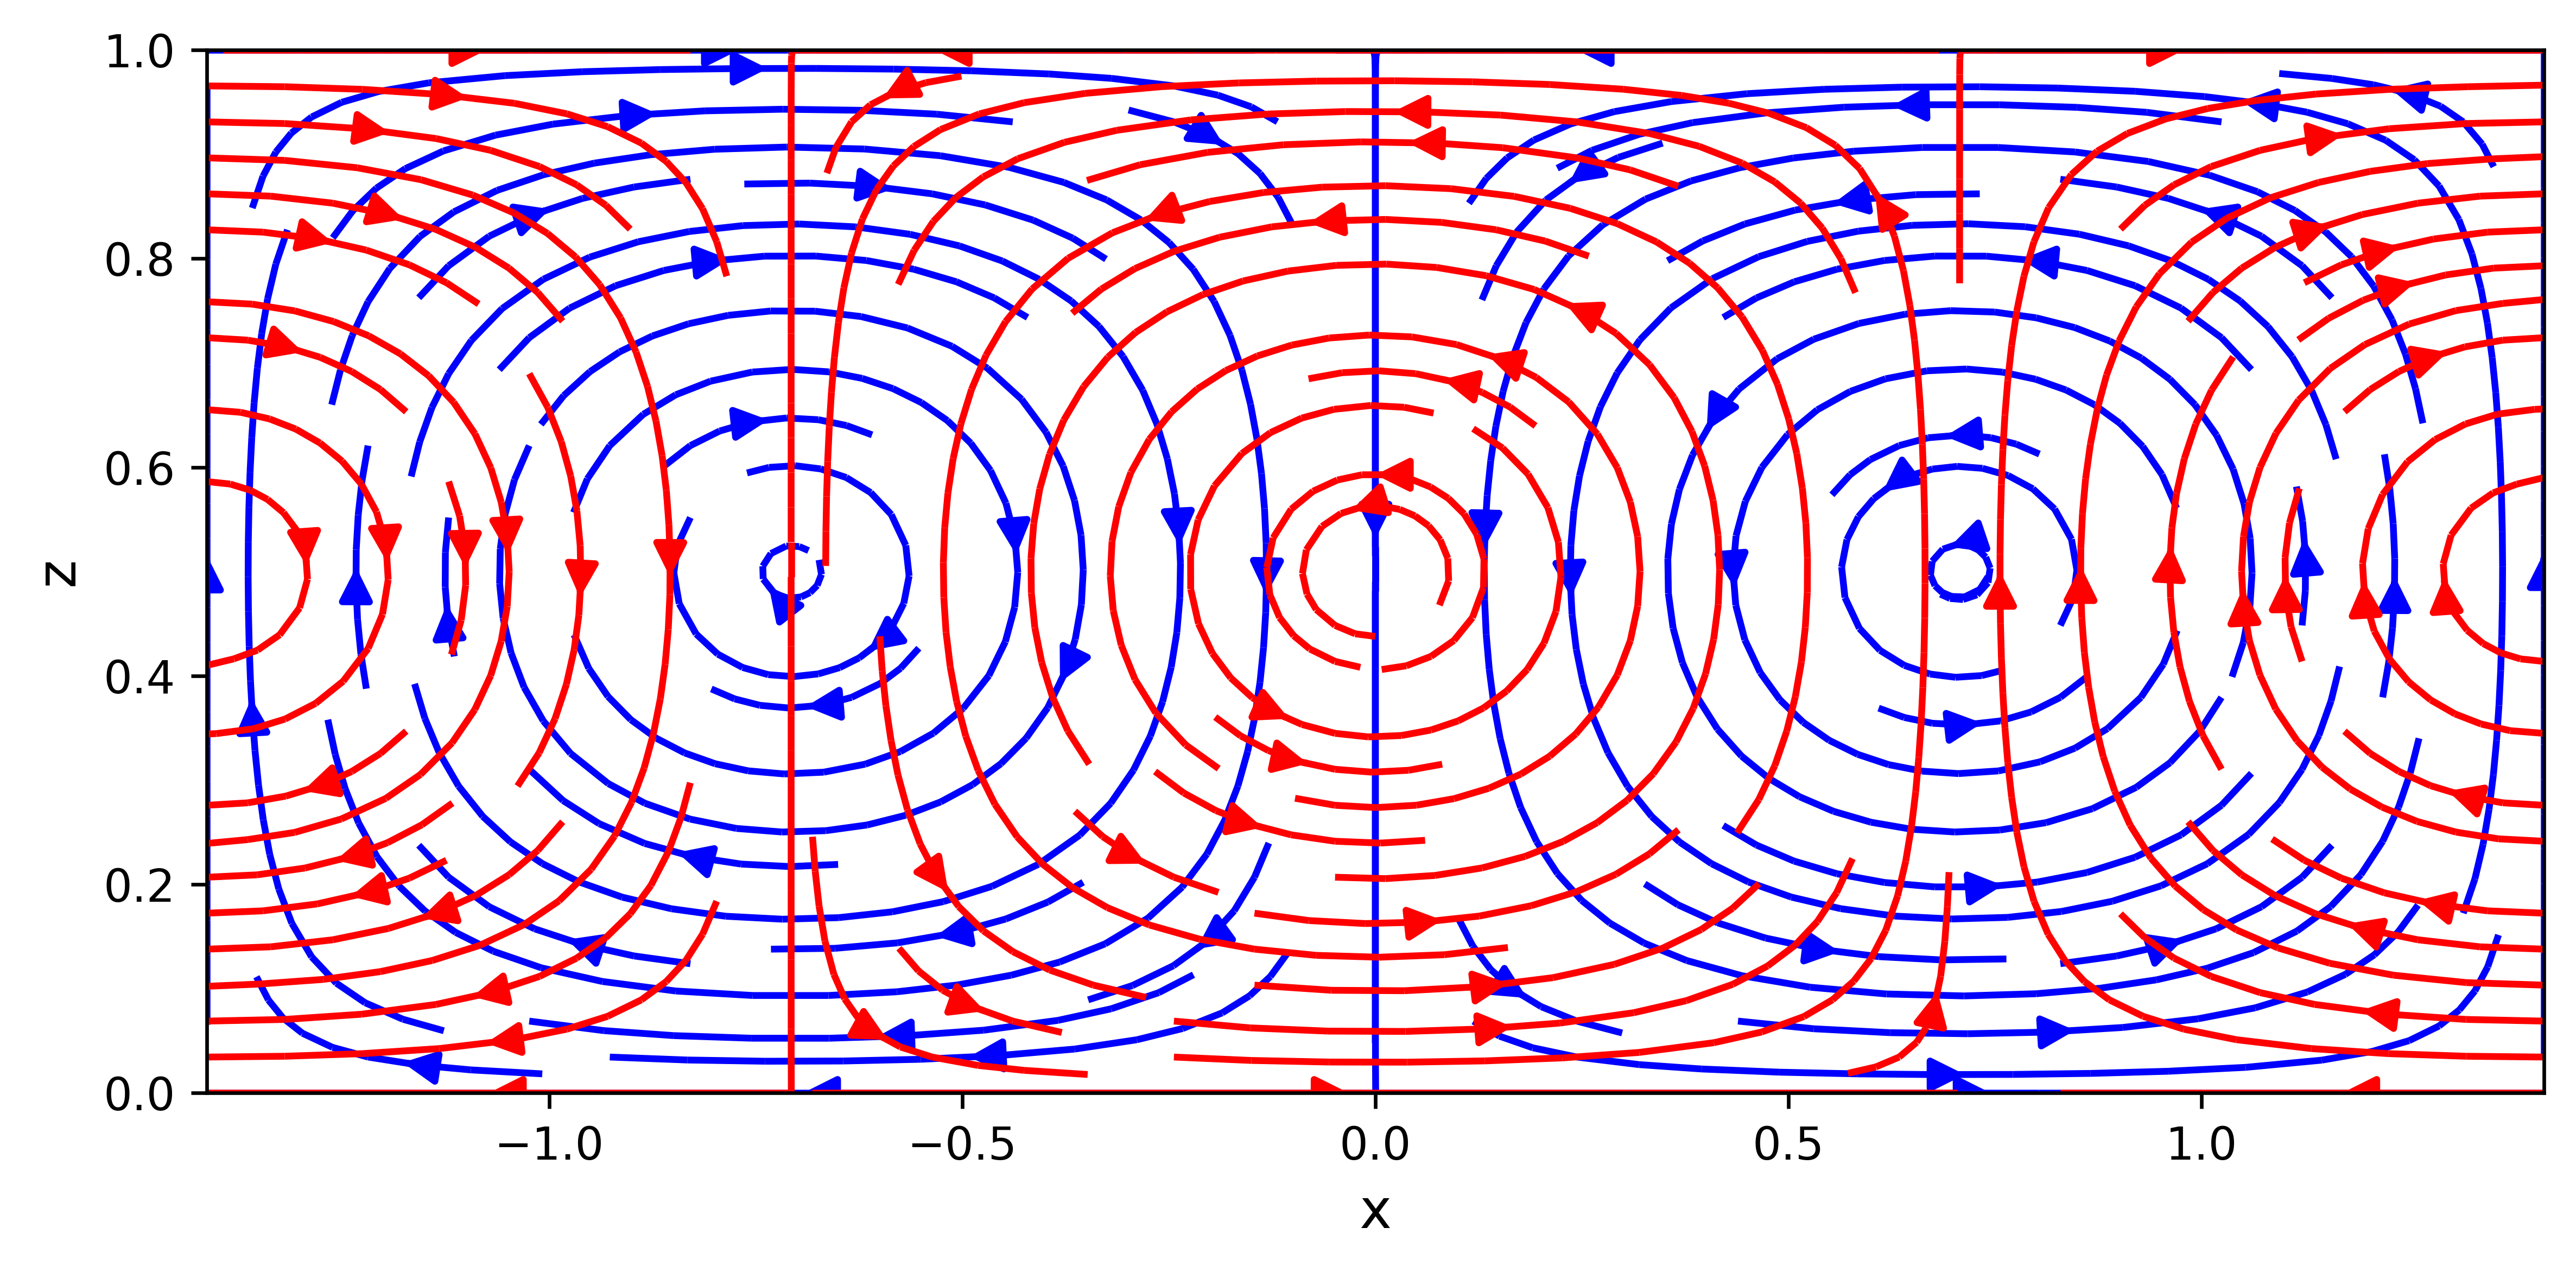
\includegraphics[width=0.9\textwidth]{media/extendedstreamlines.png}
	\caption{Streamlines for $\psi = sin \, kx \, sin \, \pi z$ (blue) and $\psi = cos \, kx \, sin \, \pi z$ (red).}
	\label{fig:extendedstreamlines}
\end{figure}


\begin{figure}[hbt!]
	\centering
	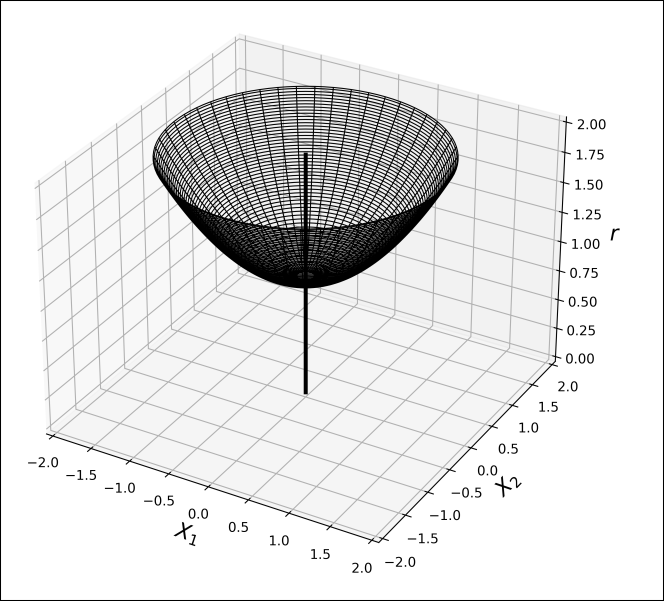
\includegraphics[width=0.7\textwidth]{media/extendedbifurcationdiagram.png}
	\caption{Partial bifurcation diagram for the extended Lorenz system.}
	\label{fig:extbifurcationdiag}
\end{figure}

Thus, the eigenvalues behave similarly to those of the Lorenz system, as shown in Figure \ref{fig:origineigs}. In particular, the base state is stable for $r<1$ and becomes unstable for $r>1$. At $r=1$, the stable attractor described in \ref{circfp} emerges. This attractor corresponds to a family of steady states representing patterns of consecutive convective rolls, with an arbitrary phase shift that preserves translational symmetry. A schematic of this is shown in Figure \ref{fig:extendedstreamlines}. Figure \ref{fig:extbifurcationdiag} presents a partial bifurcation diagram illustrating the emergence of this attractor. A cross-section of this diagram recovers the bifurcation behavior of the classical Lorenz system.\\

\noindent The Jacobian matrix at any of these fixed points is given by
\begin{equation}
J = \begin{bmatrix}
	-\sigma & 0 & \sigma & 0 & 0 \\
	0 & -\sigma & 0 & -\sigma & 0 \\
	1 & 0 & -1 & 0 & -\sqrt{b (r - 1)} \cos \, \omega \\
	0 & -1 & 0 & -1 & \sqrt{b (r - 1)} \sin \, \omega \\
	\sqrt{b (r - 1)} \cos \, \omega & \sqrt{b (r - 1)} \sin \, \omega & \sqrt{b (r - 1)} \cos \, \omega & -\sqrt{b (r - 1)} \sin \, \omega & -b
\end{bmatrix}
\end{equation}\\

Figure \ref{fig:exthopf_eigs} shows how the real and imaginary parts of the eigenvalues evolve as the parameter $r$ varies. There is always a zero eigenvalue, which arises due to the degeneracy of the fixed points, as they lie on a continuous circle. The other eigenvalues behave similarly to those in the Lorenz system, but with the addition of a real negative eigenvalue. This suggests that the attractor, consisting of fixed points, exhibits neutral stability along the direction of the circle (due to the zero eigenvalue) and is stable in all other directions for $r < 24.74$. Above this threshold, the attractor loses its stability and the system becomes chaotic.\\

\begin{figure}[hbt!]
	\centering
	
	\begin{subfigure}[b]{0.49\textwidth}
		\centering
		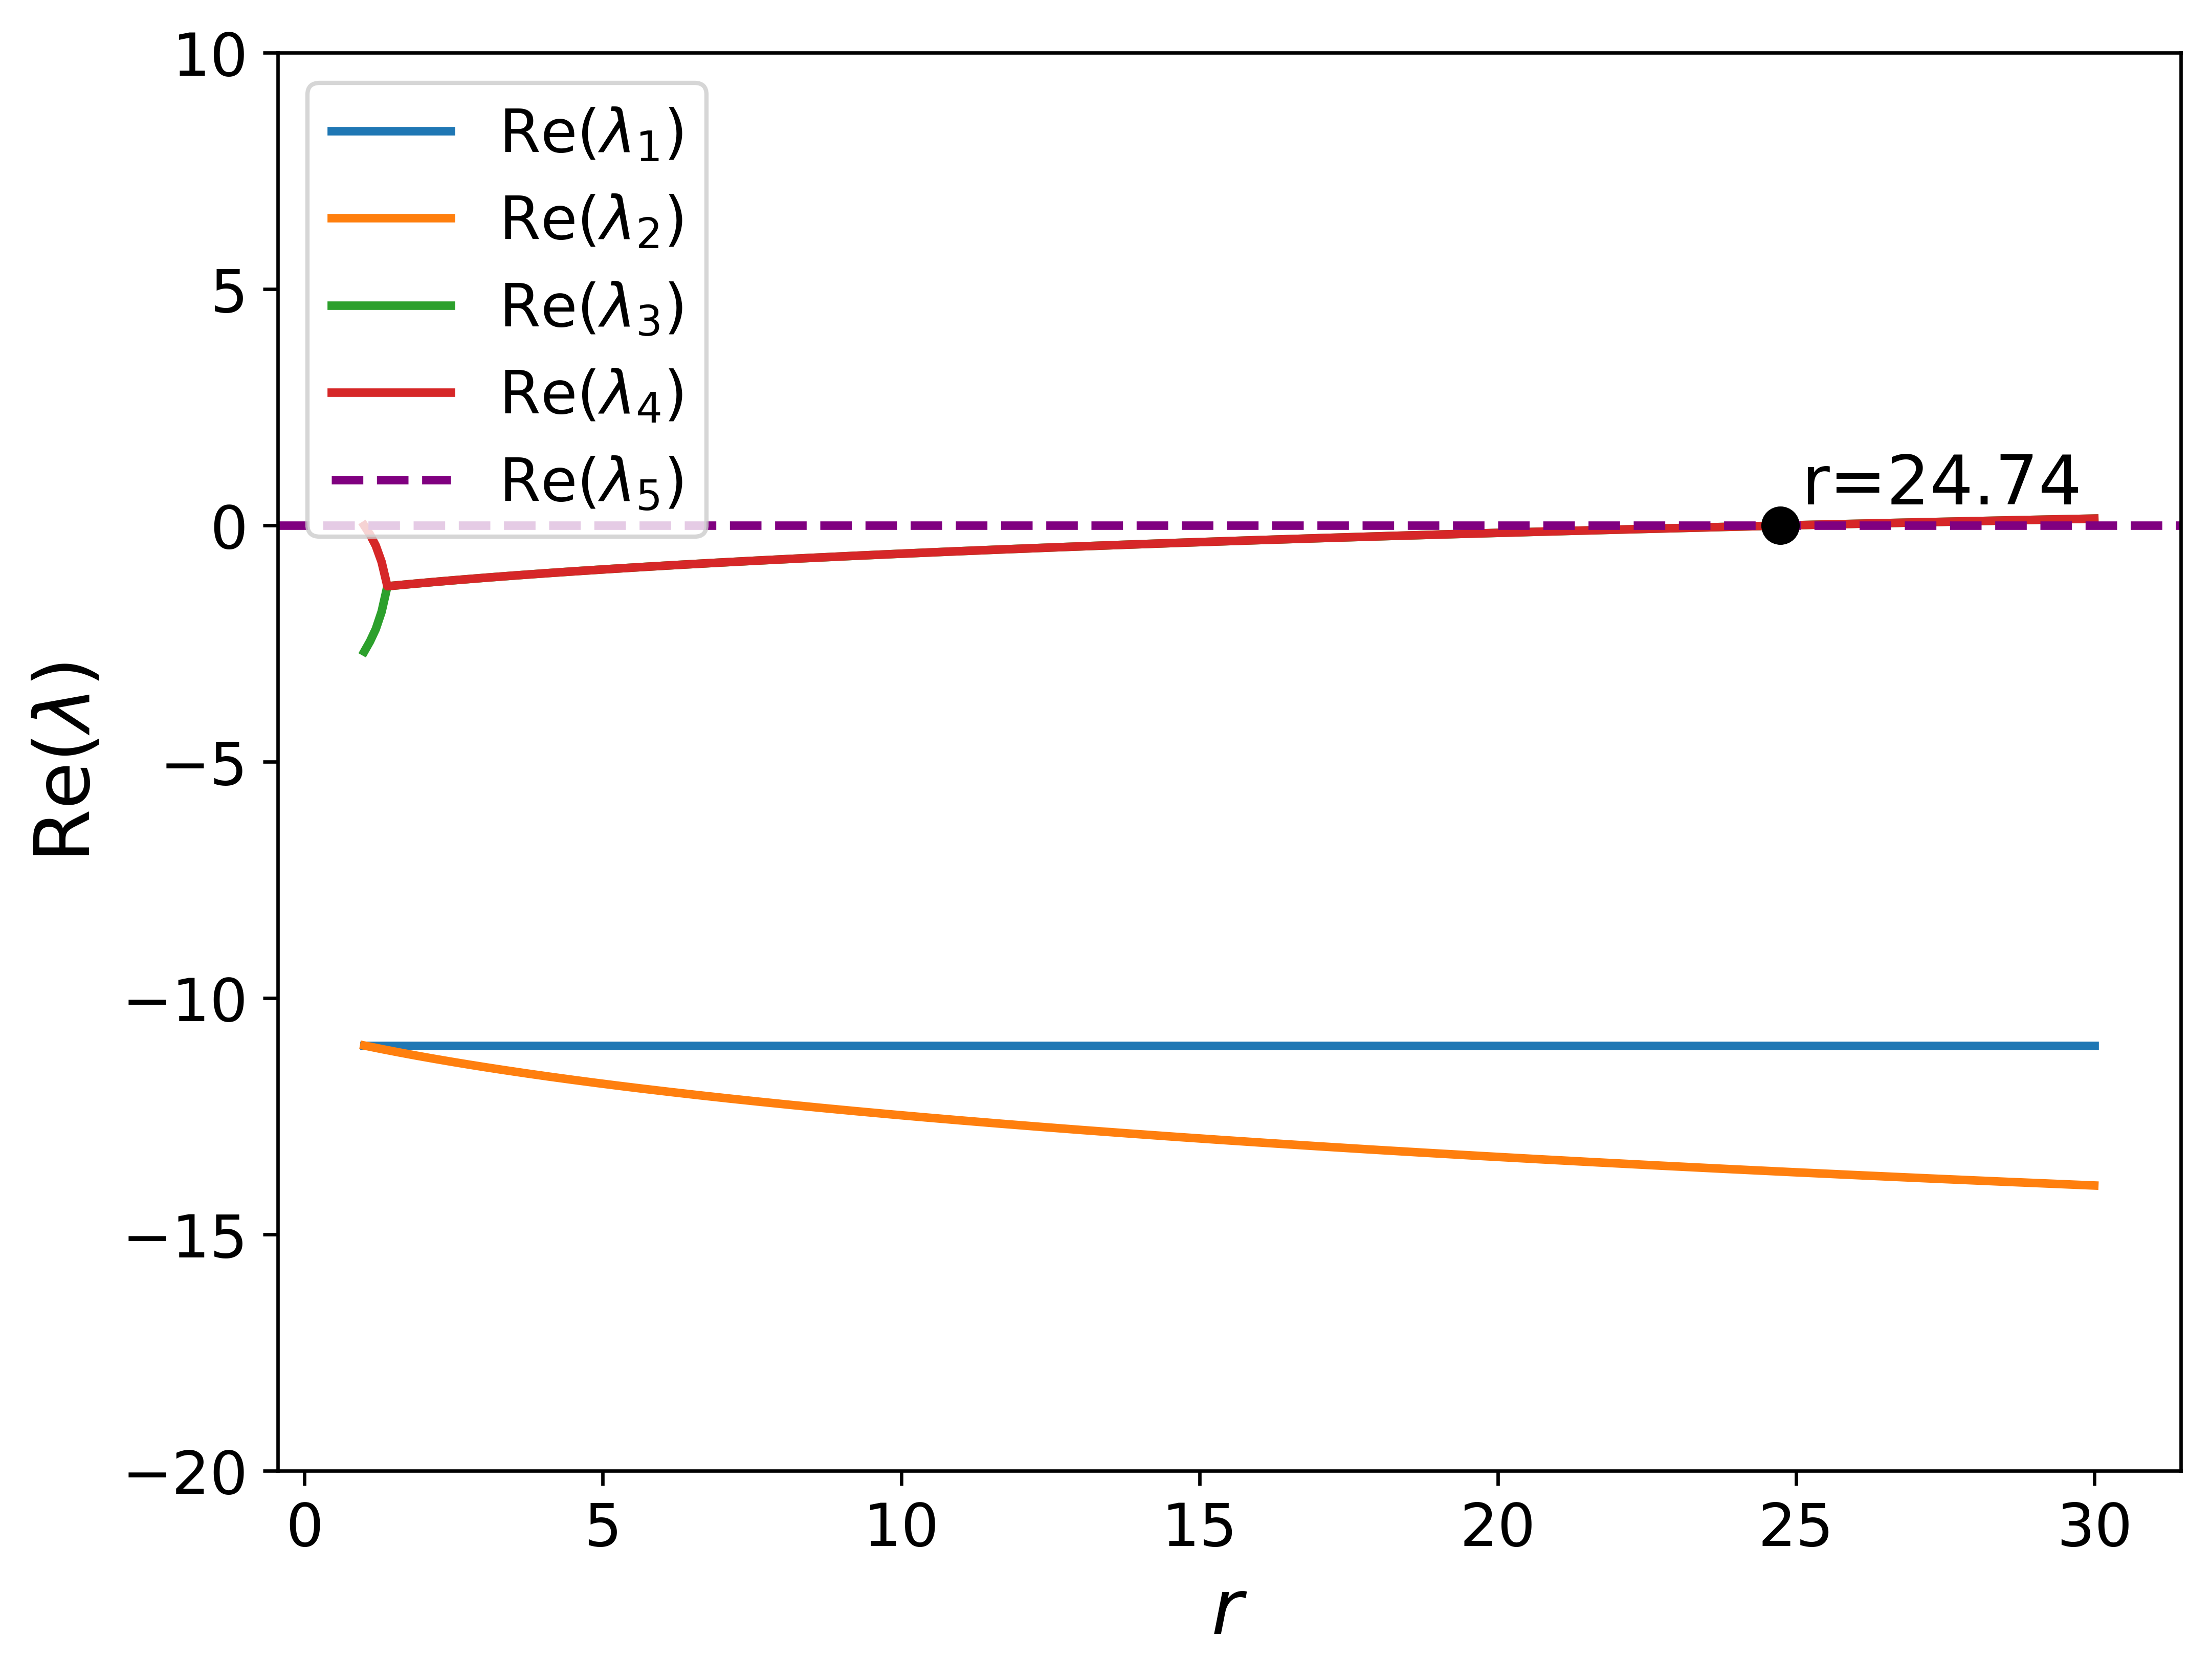
\includegraphics[width=\textwidth]{media/extendedhopf_eigs_real.png}
		\caption{}
		\label{fig:sub1}
	\end{subfigure}
	\hfill
	\begin{subfigure}[b]{0.49\textwidth}
		\centering
		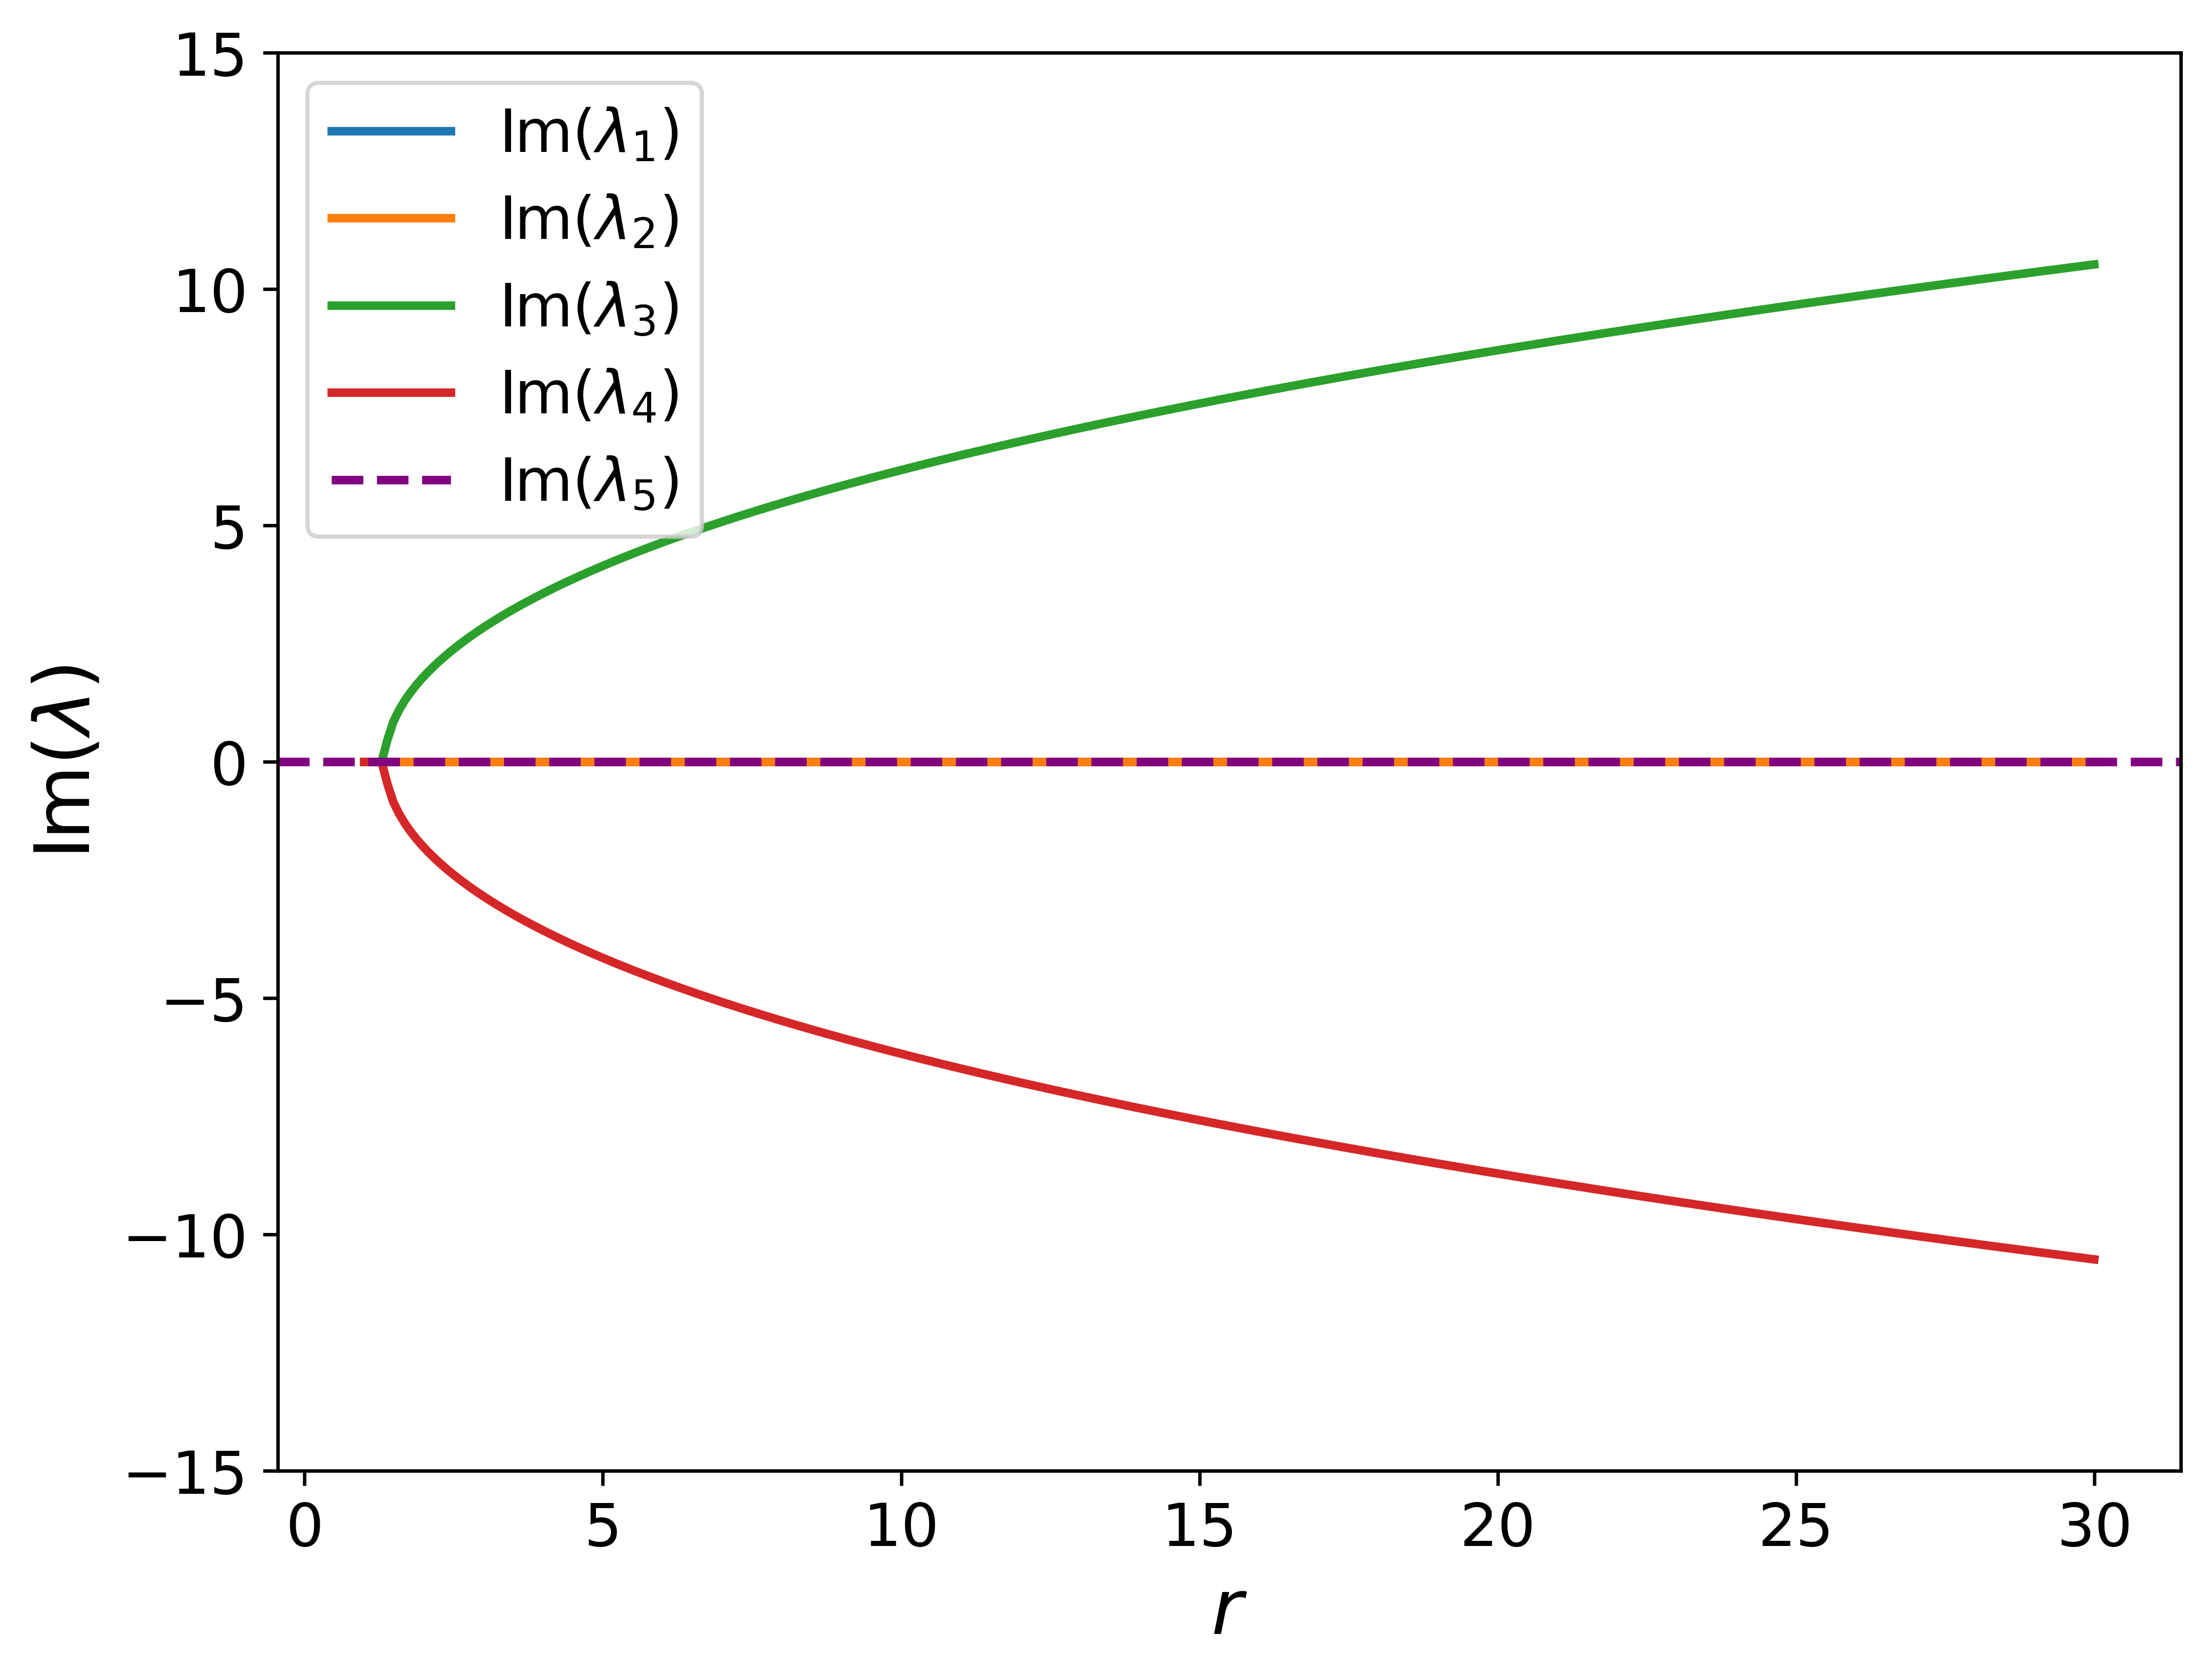
\includegraphics[width=\textwidth]{media/extendedhopf_eigs_imag.png}
		\caption{}
		\label{fig:sub2}
	\end{subfigure}
	
	\caption{Real and imaginary parts of the eigenvalues of the fixed points on the attractor for the extended Lorenz system versus the parameter $r$.}
	\label{fig:exthopf_eigs}
\end{figure}

\subsection{Geometry of the Strange Attractor}
\noindent Consider a trajectory originating at a point 
\begin{equation}
	\begin{split}
		&X_1 = X_0 \, cos \, \omega \qquad X_2 = X_0 \, sin \, \omega \\
		& \; Y_1 = Y_0 \, cos \, \omega \qquad Y_2 = - Y_0 \, sin \, \omega \\
		& \qquad  Z = Z_0 \qquad \qquad  0 \leq \omega \leq 2 \, \pi
	\end{split} 
	\label{init}
\end{equation}

\noindent Substituting in \ref{extlrzx1}-\ref{extlrzz}, we get
\begin{equation}
	\dot{X_1} =  \sigma \, (-X_0 + Y_0) \, cos \, \omega
	\label{extlrzx1inv}
\end{equation}
\begin{equation}
	\dot{X_2} =  \sigma \, (-X_0 + Y_0) \, sin \, \omega
	\label{extlrzx2inv}
\end{equation}
\begin{equation}
	\dot{Y_1} = (-X_0 \, Z_0 + r \, X_0 - Y_0) \, cos \, \omega
	\label{extlrzy1inv}
\end{equation}
\begin{equation}
	\dot{Y_2} = -(-X_0 \, Z_0 + r \, X_0 - Y_0) \, sin \, \omega
	\label{extlrzy2inv}
\end{equation}
\begin{equation}
	\dot{Z} = X_0 \, Y_0 - b \, Z
	\label{extlrzzinv}
\end{equation}\\

Equations \ref{extlrzx1inv}–\ref{extlrzzinv} satisfy $d(X_1/X_2)/dt = d(Y_1/Y_2)/dt = 0$, implying that the ratios $X_1/X_2$ and $Y_1/Y_2$ remain constant along trajectories. Consequently, the dynamics starting from an initial condition of the form \eqref{init} are confined to a lower-dimensional invariant set — meaning trajectories starting in this set remain within it for all time.\\

Importantly, for each fixed value of $\omega$, the governing equations \ref{extlrzx1inv}–\ref{extlrzzinv} reduce to the Lorenz system equations, with $(X_0, Y_0, Z_0)$ playing the role of the Lorenz system variables. Thus, for every value of $\omega \in [0, 2\pi]$, the extended system contains a copy of the Lorenz system embedded within it. In this way, the Lorenz system appears as a continuous family of invariant subsets in the extended system.\\

Therefore, the projection of the chaotic attractor of the extended Lorenz system in the $X_1-X_2-Z$ space forms a volume of revolution of the Lorenz attractor in the $X-Z$ plane. The same holds for the $Y_1-Y_2-Z$ projection. This geometric structure is illustrated in Figure \ref{fig:extendedattractor}.\\
	
\begin{figure}[hbt!]
	\centering
	\begin{subfigure}[b]{0.495\textwidth}
		\centering
		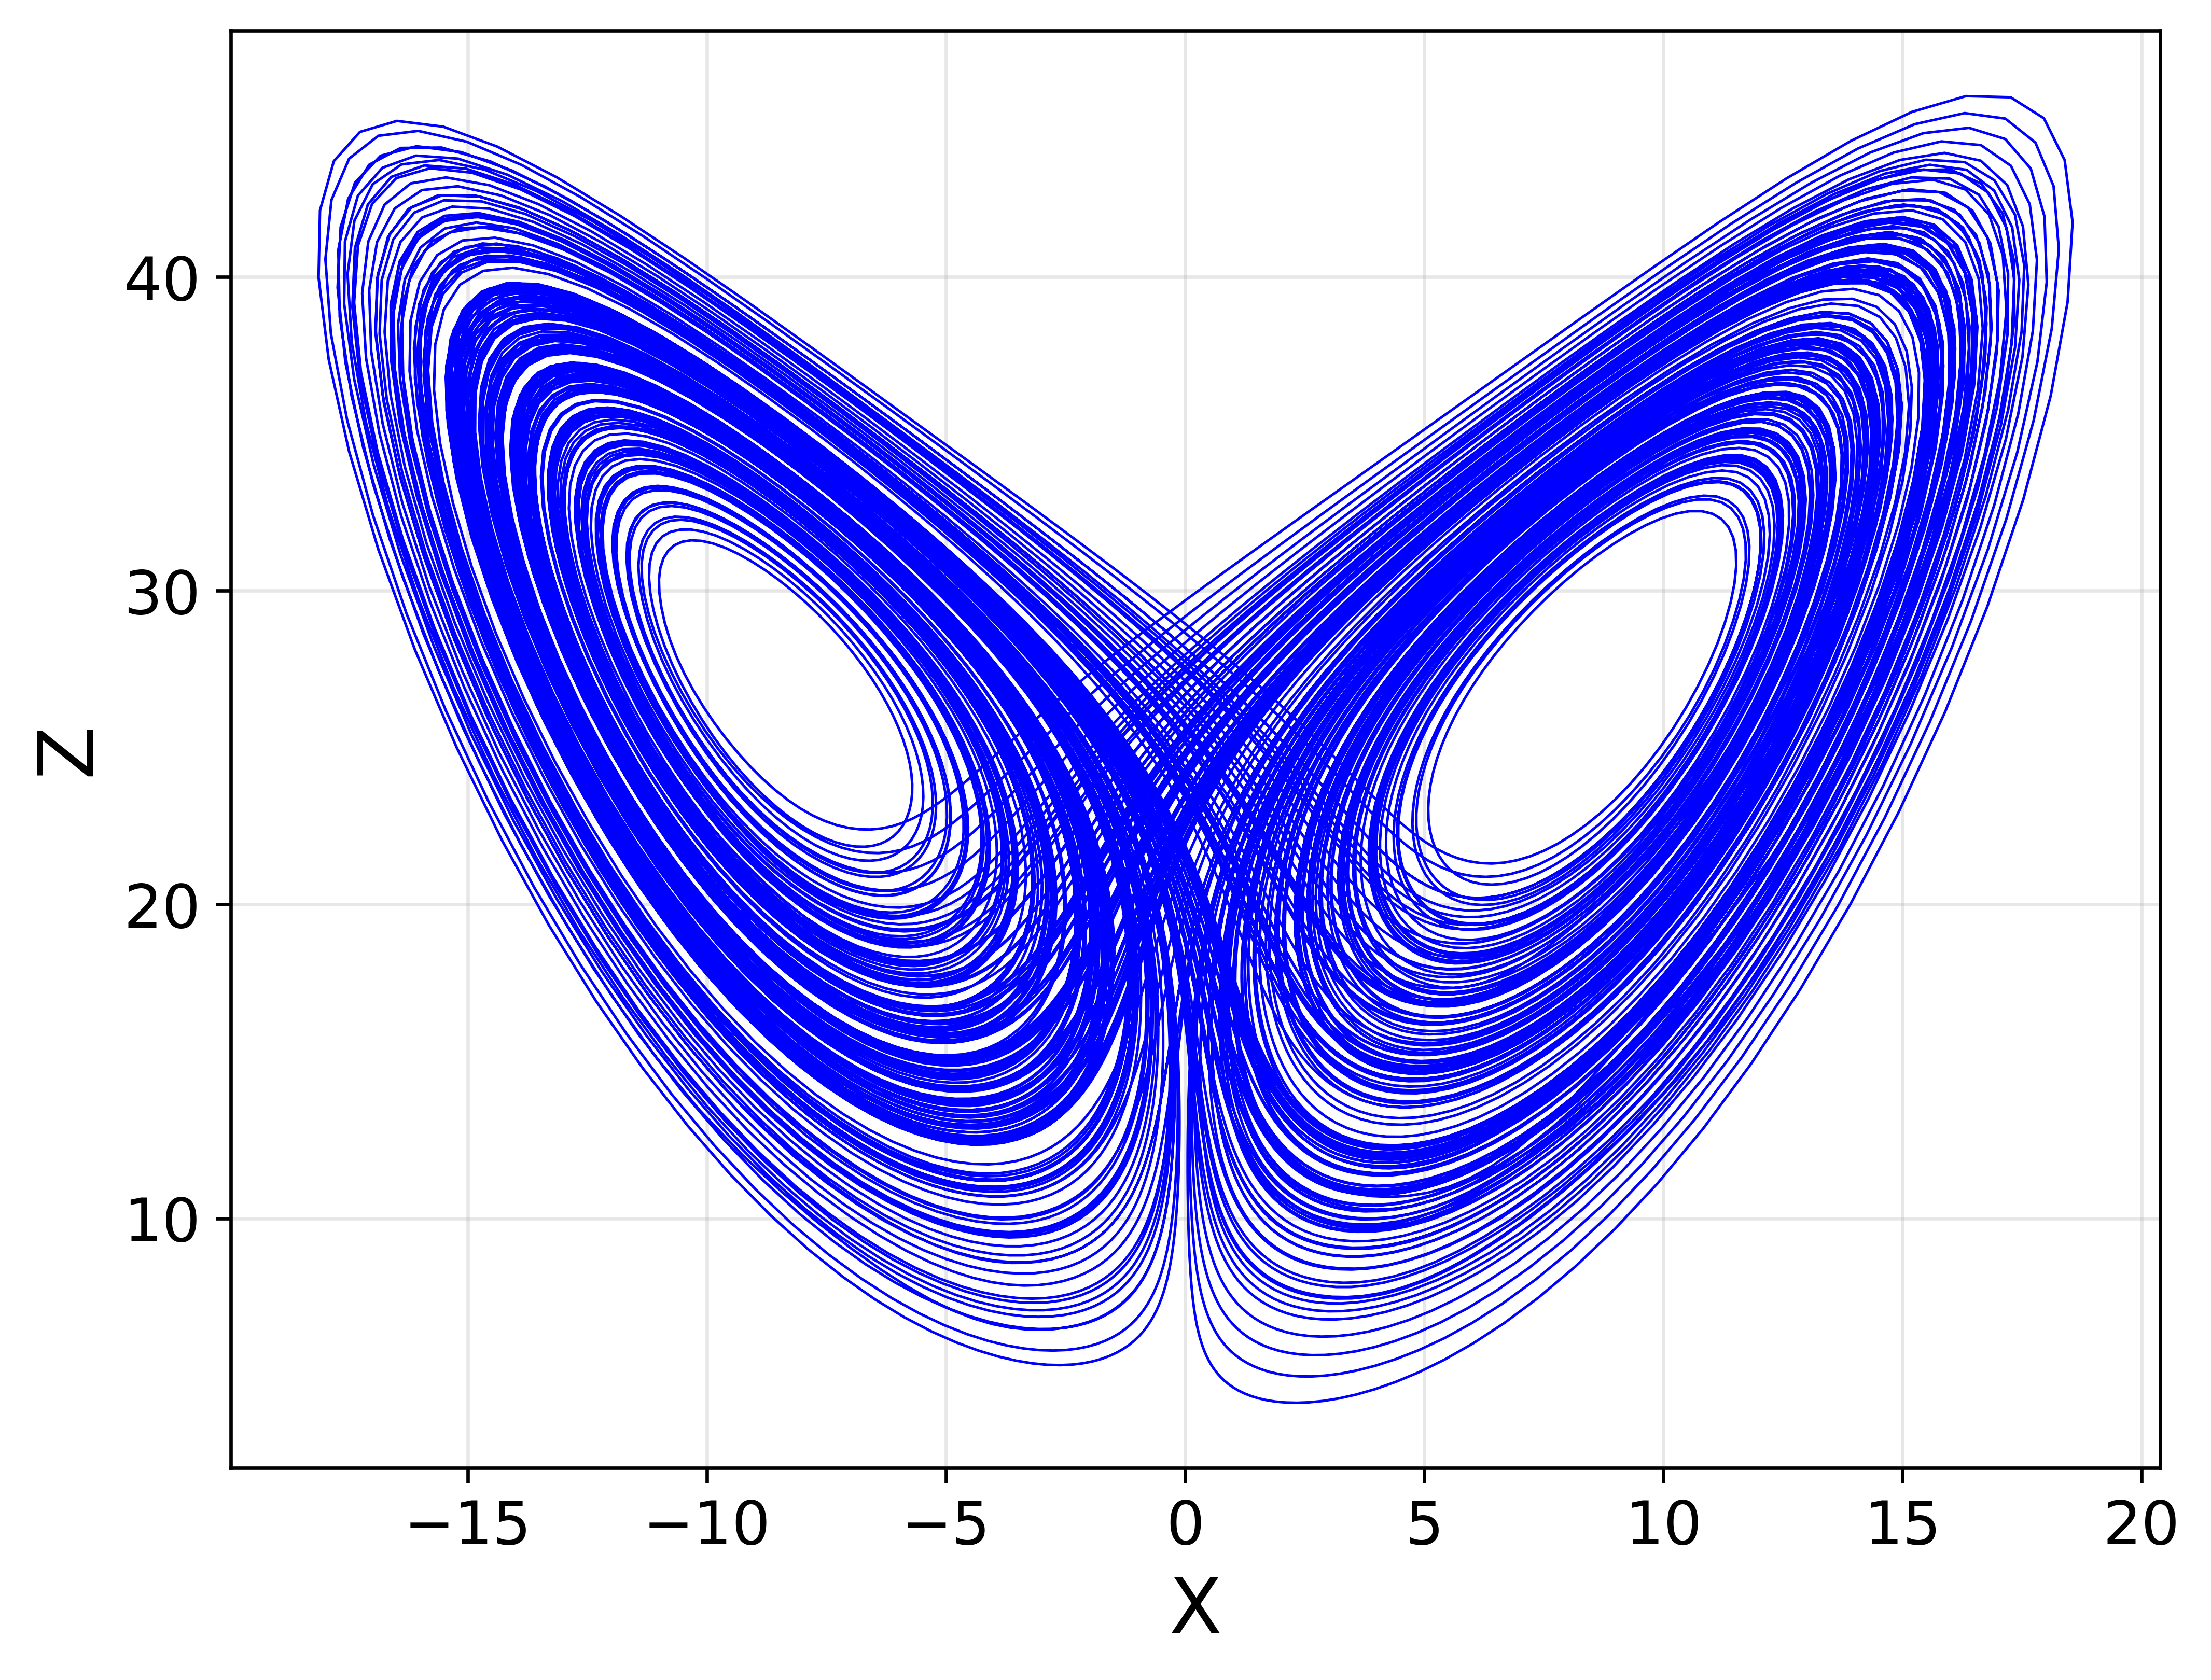
\includegraphics[width=\textwidth]{media/lorenz_xz_projection.png}
		\caption{}
		\label{fig:sub1}
	\end{subfigure}
	\hfill
	\begin{subfigure}[b]{0.495\textwidth}
		\centering
		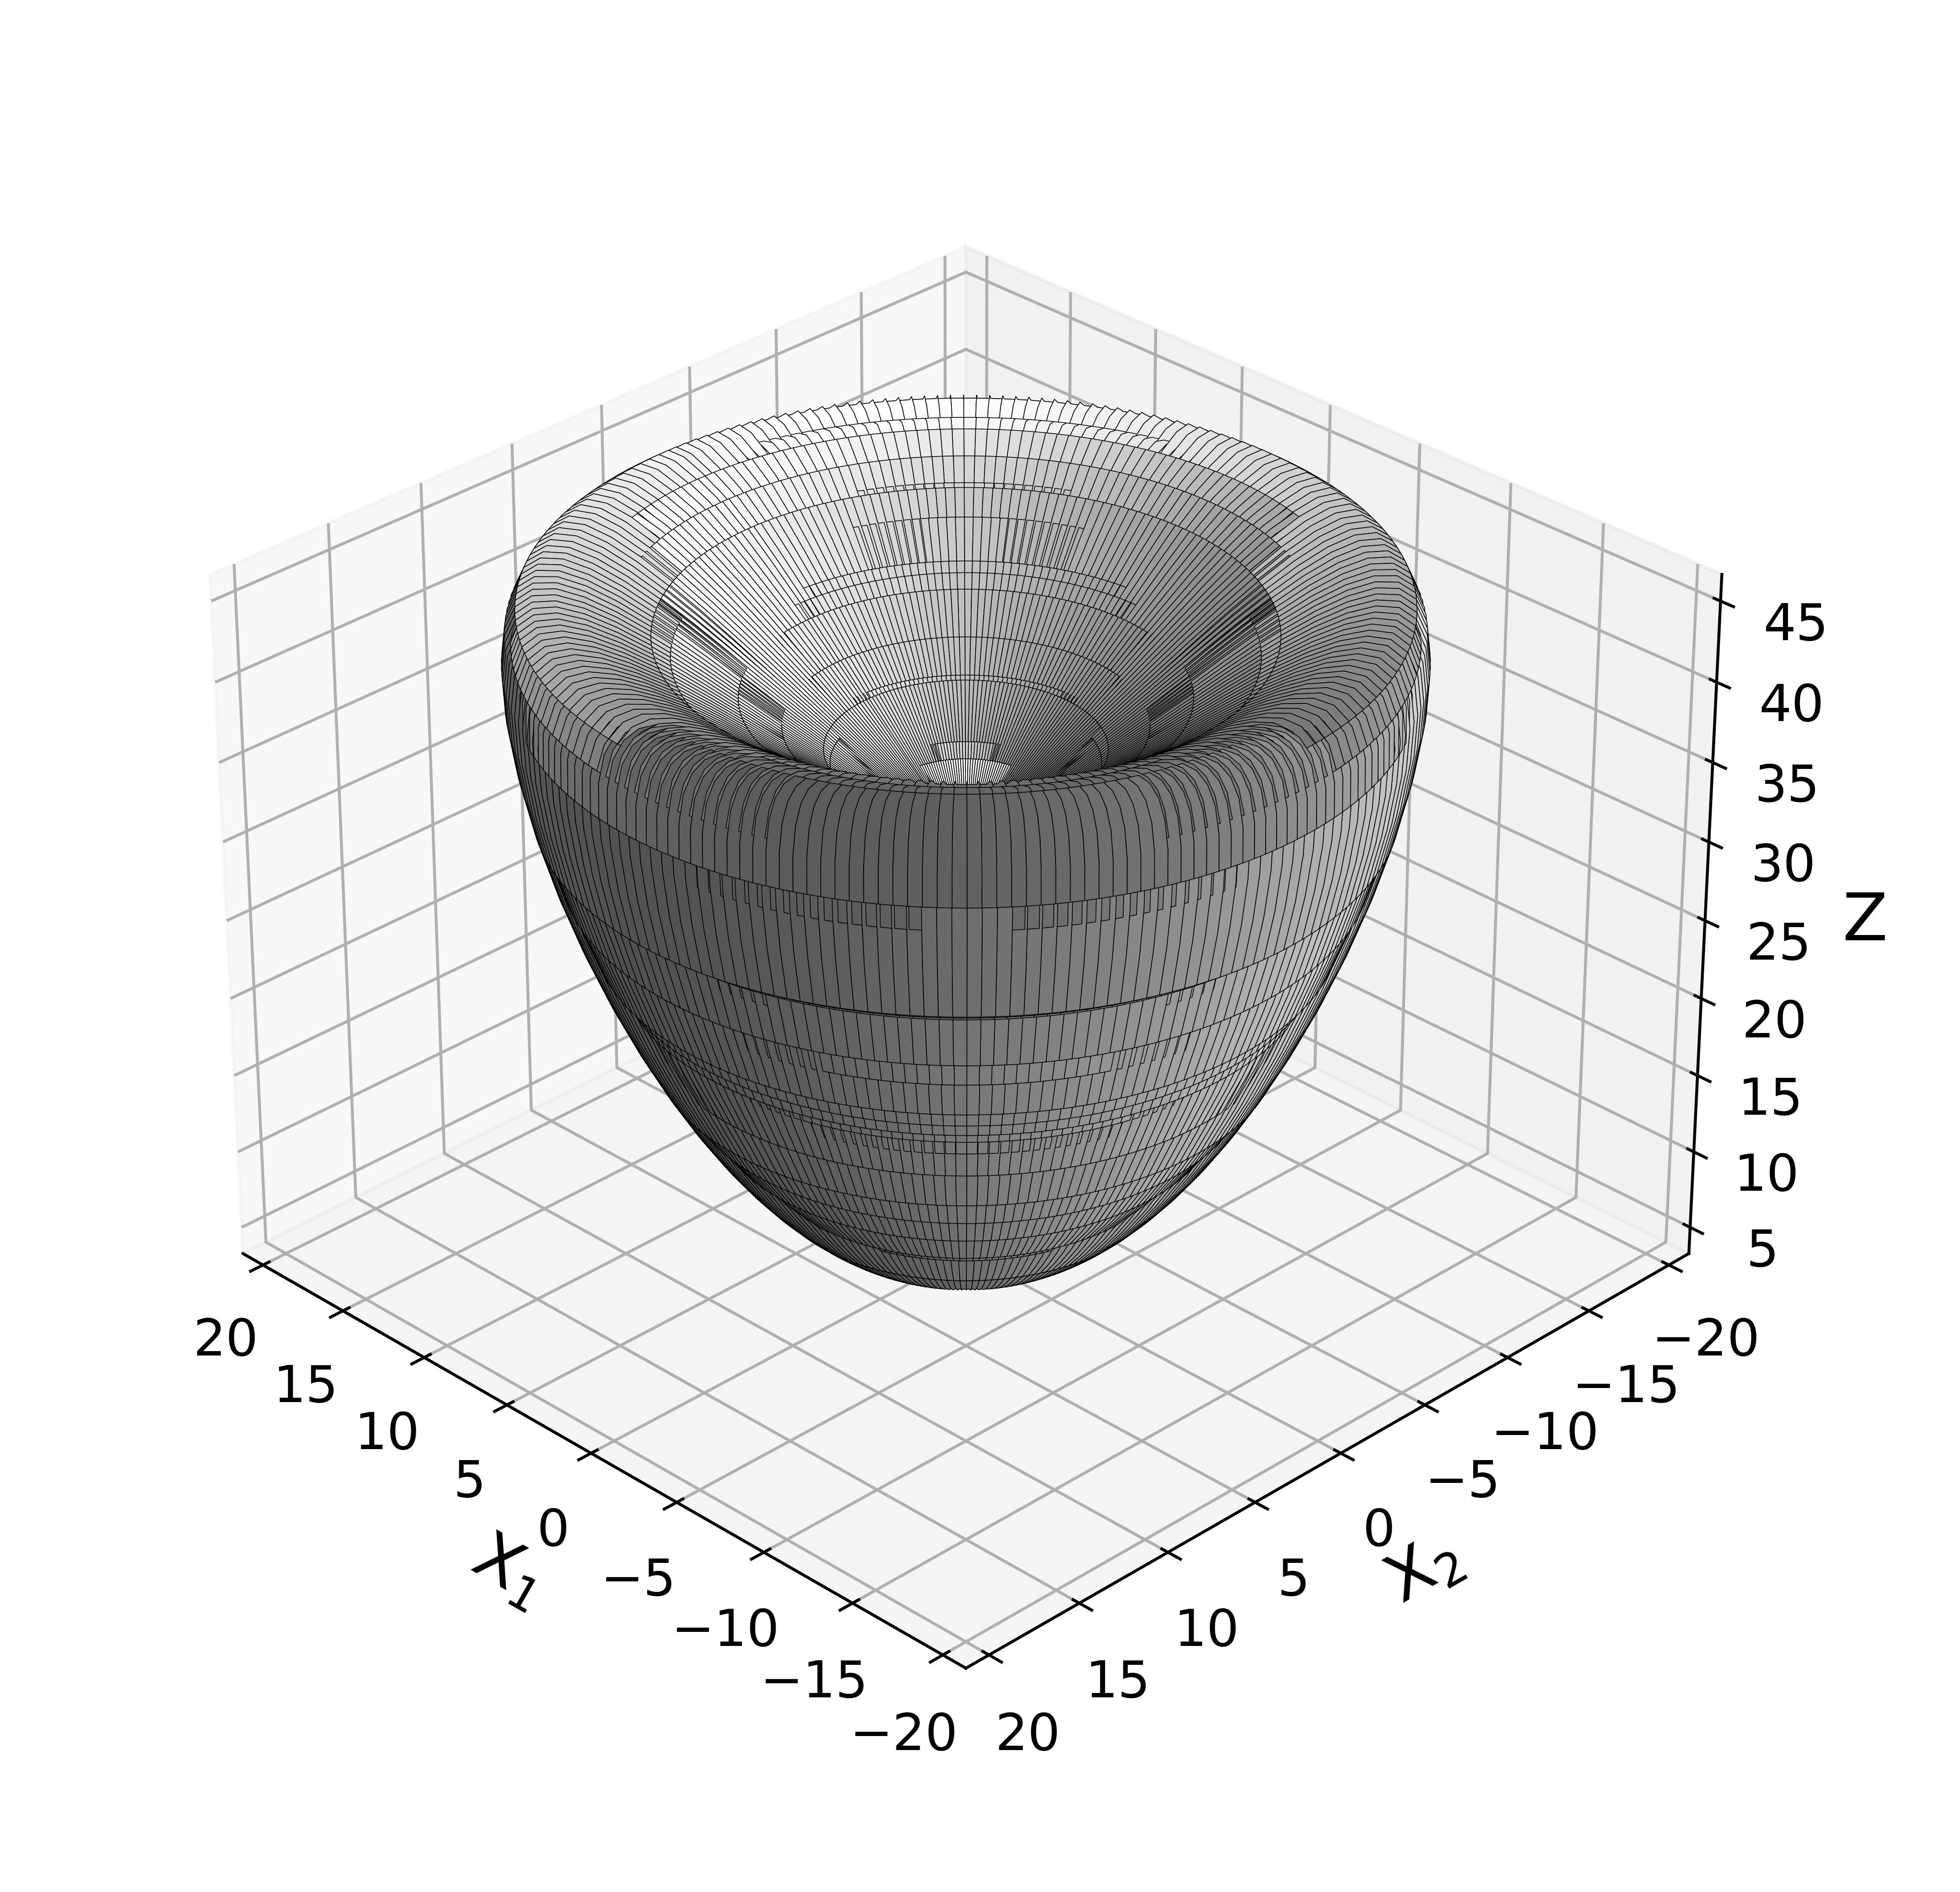
\includegraphics[width=\textwidth]{media/lorenz_surface_of_revolution.png}
		\caption{}
		\label{fig:sub2}
	\end{subfigure}
	\hfill
	\begin{subfigure}[b]{0.495\textwidth}
		\centering
		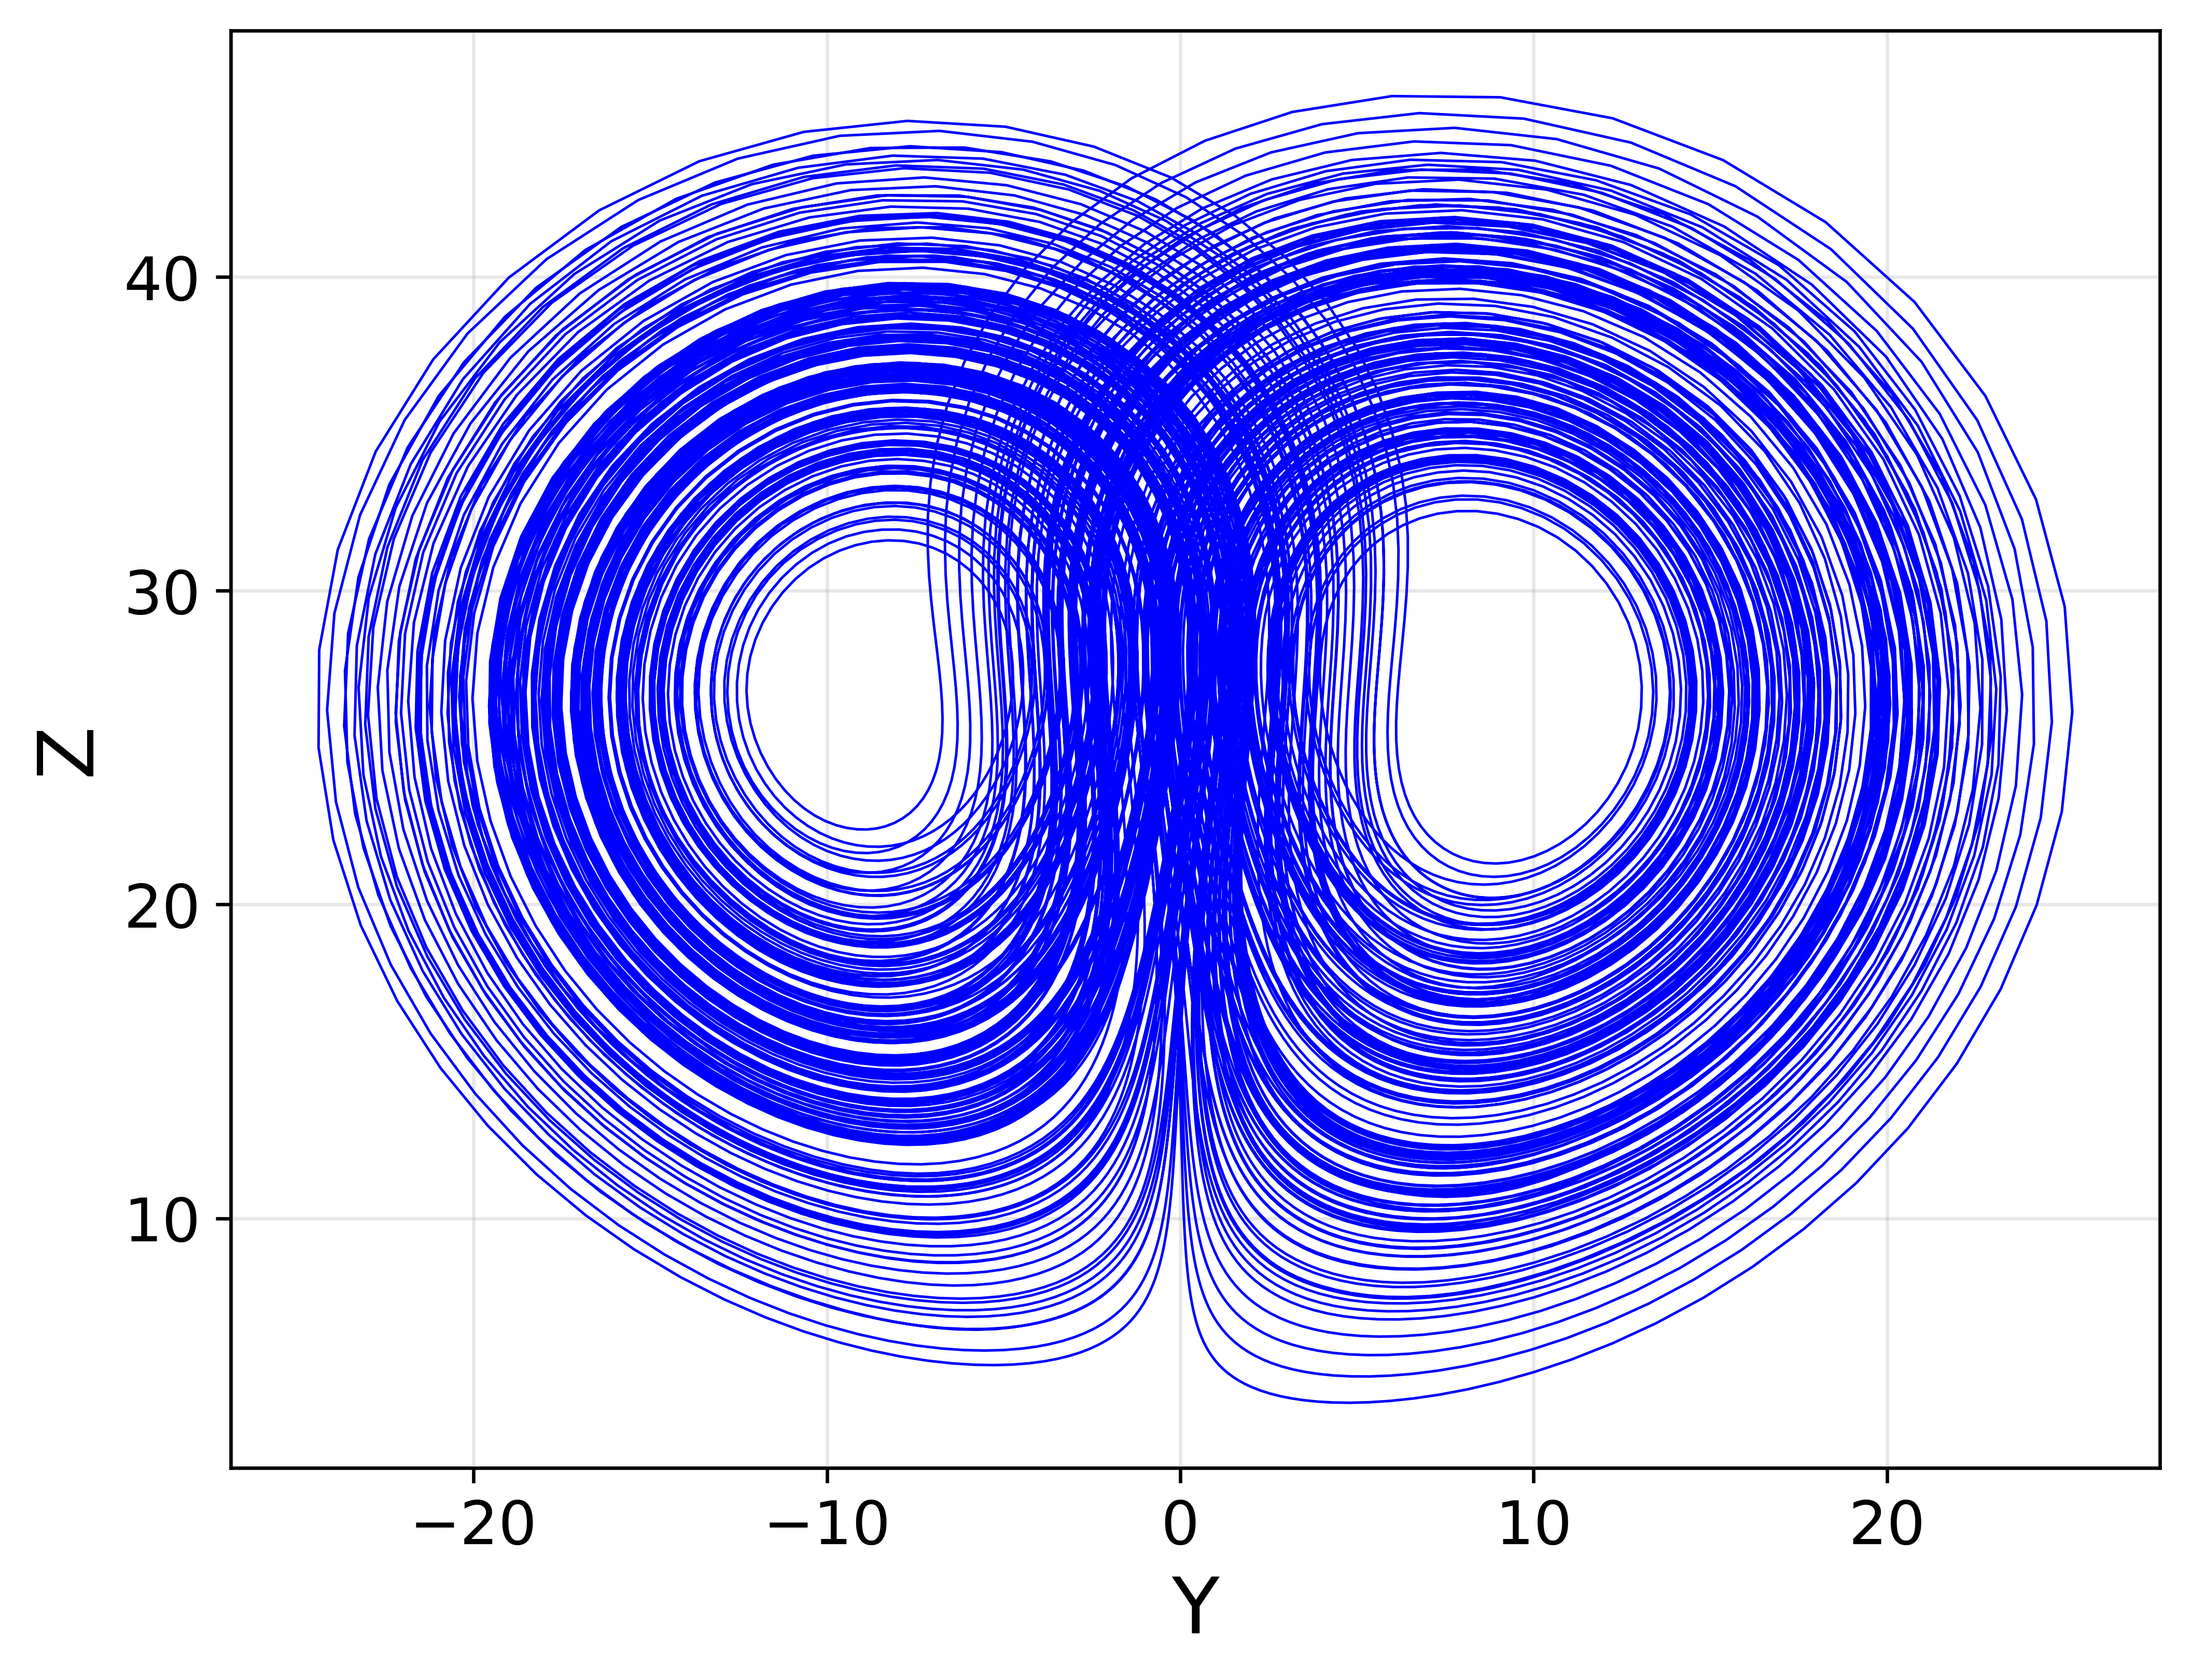
\includegraphics[width=\textwidth]{media/lorenz_yz_projection.png}
		\caption{}
		\label{fig:sub1}
	\end{subfigure}
	\hfill
	\begin{subfigure}[b]{0.495\textwidth}
		\centering
		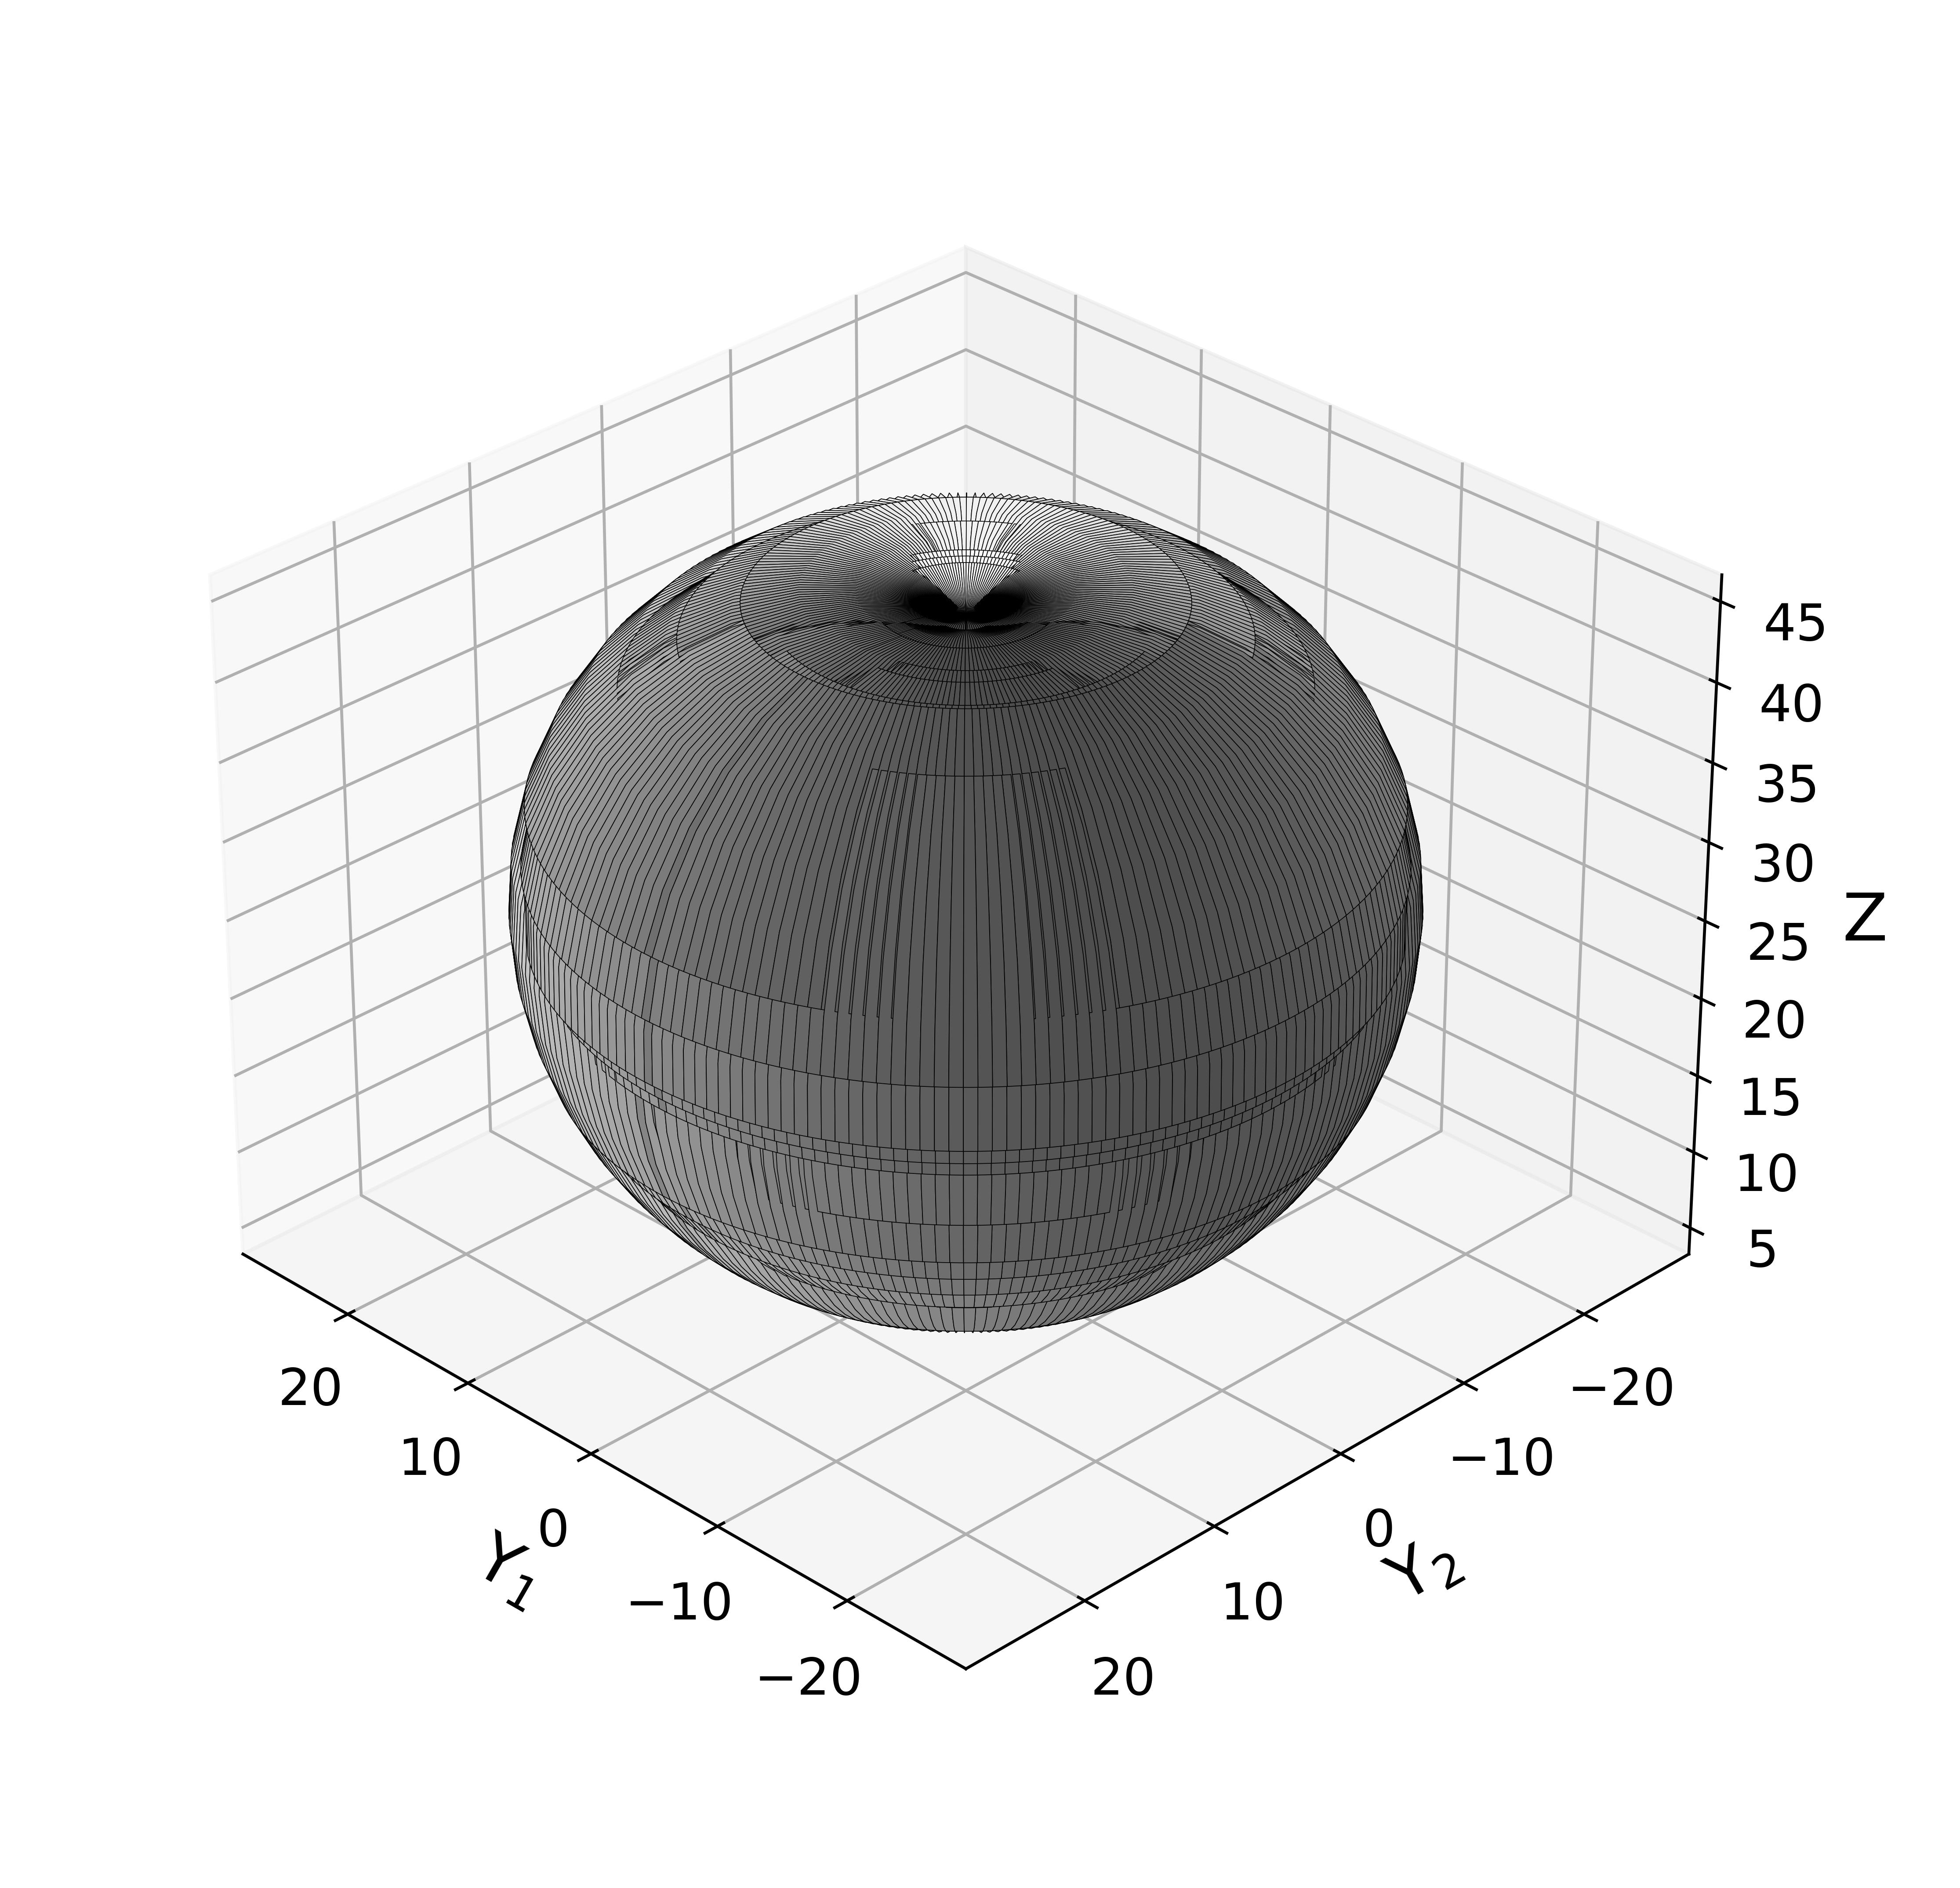
\includegraphics[width=\textwidth]{media/lorenz_y_surface_of_revolution.png}
		\caption{}
		\label{fig:sub2}
	\end{subfigure}
	
	\caption{(a and c) Projections of phase portraits of the chaotic attractor or the Lorenz system on the X-Z and Y-Z planes for $r = 28$. (b and d) Solids of revolution of the phase portraits of the Lorenz system about the Z-axis visualizing the attractor of the extended Lorenz system.}
	\label{fig:extendedattractor}
\end{figure}
	
Although the projections of the attractor in the \( X_1\text{--}X_2\text{--}Z \) and \( Y_1\text{--}Y_2\text{--}Z \) spaces appear fully three-dimensional, the entire attractor is not explored by individual trajectories. This is evident in Figure~\ref{fig:extendedsimulations}, which shows the system’s evolution for two different initial conditions. The trajectories, though not initially lying on an invariant set, rapidly settle onto one within a short time and remain confined to it thereafter. Thus, the long-term dynamics unfold on a lower-dimensional invariant manifold of the full attractor. The ratios \( X_1/X_2 \) and \( -Y_1/Y_2 \) stabilize to constant values, uniquely characterizing the invariant manifold on which the trajectory resides. Physically, in the context of the convection problem, this implies that a specific spatial pattern of convective rolls establishes itself early on, and only the strength and direction of the roll circulation continue to vary aperiodically with time. This spatial pattern is determined by the initial conditions and can vary from one trajectory to another—unlike in the classical Lorenz system, where the spatial pattern is fixed.

\begin{figure}[hbt!]
	\centering
	\begin{subfigure}[b]{0.495\textwidth}
		\centering
		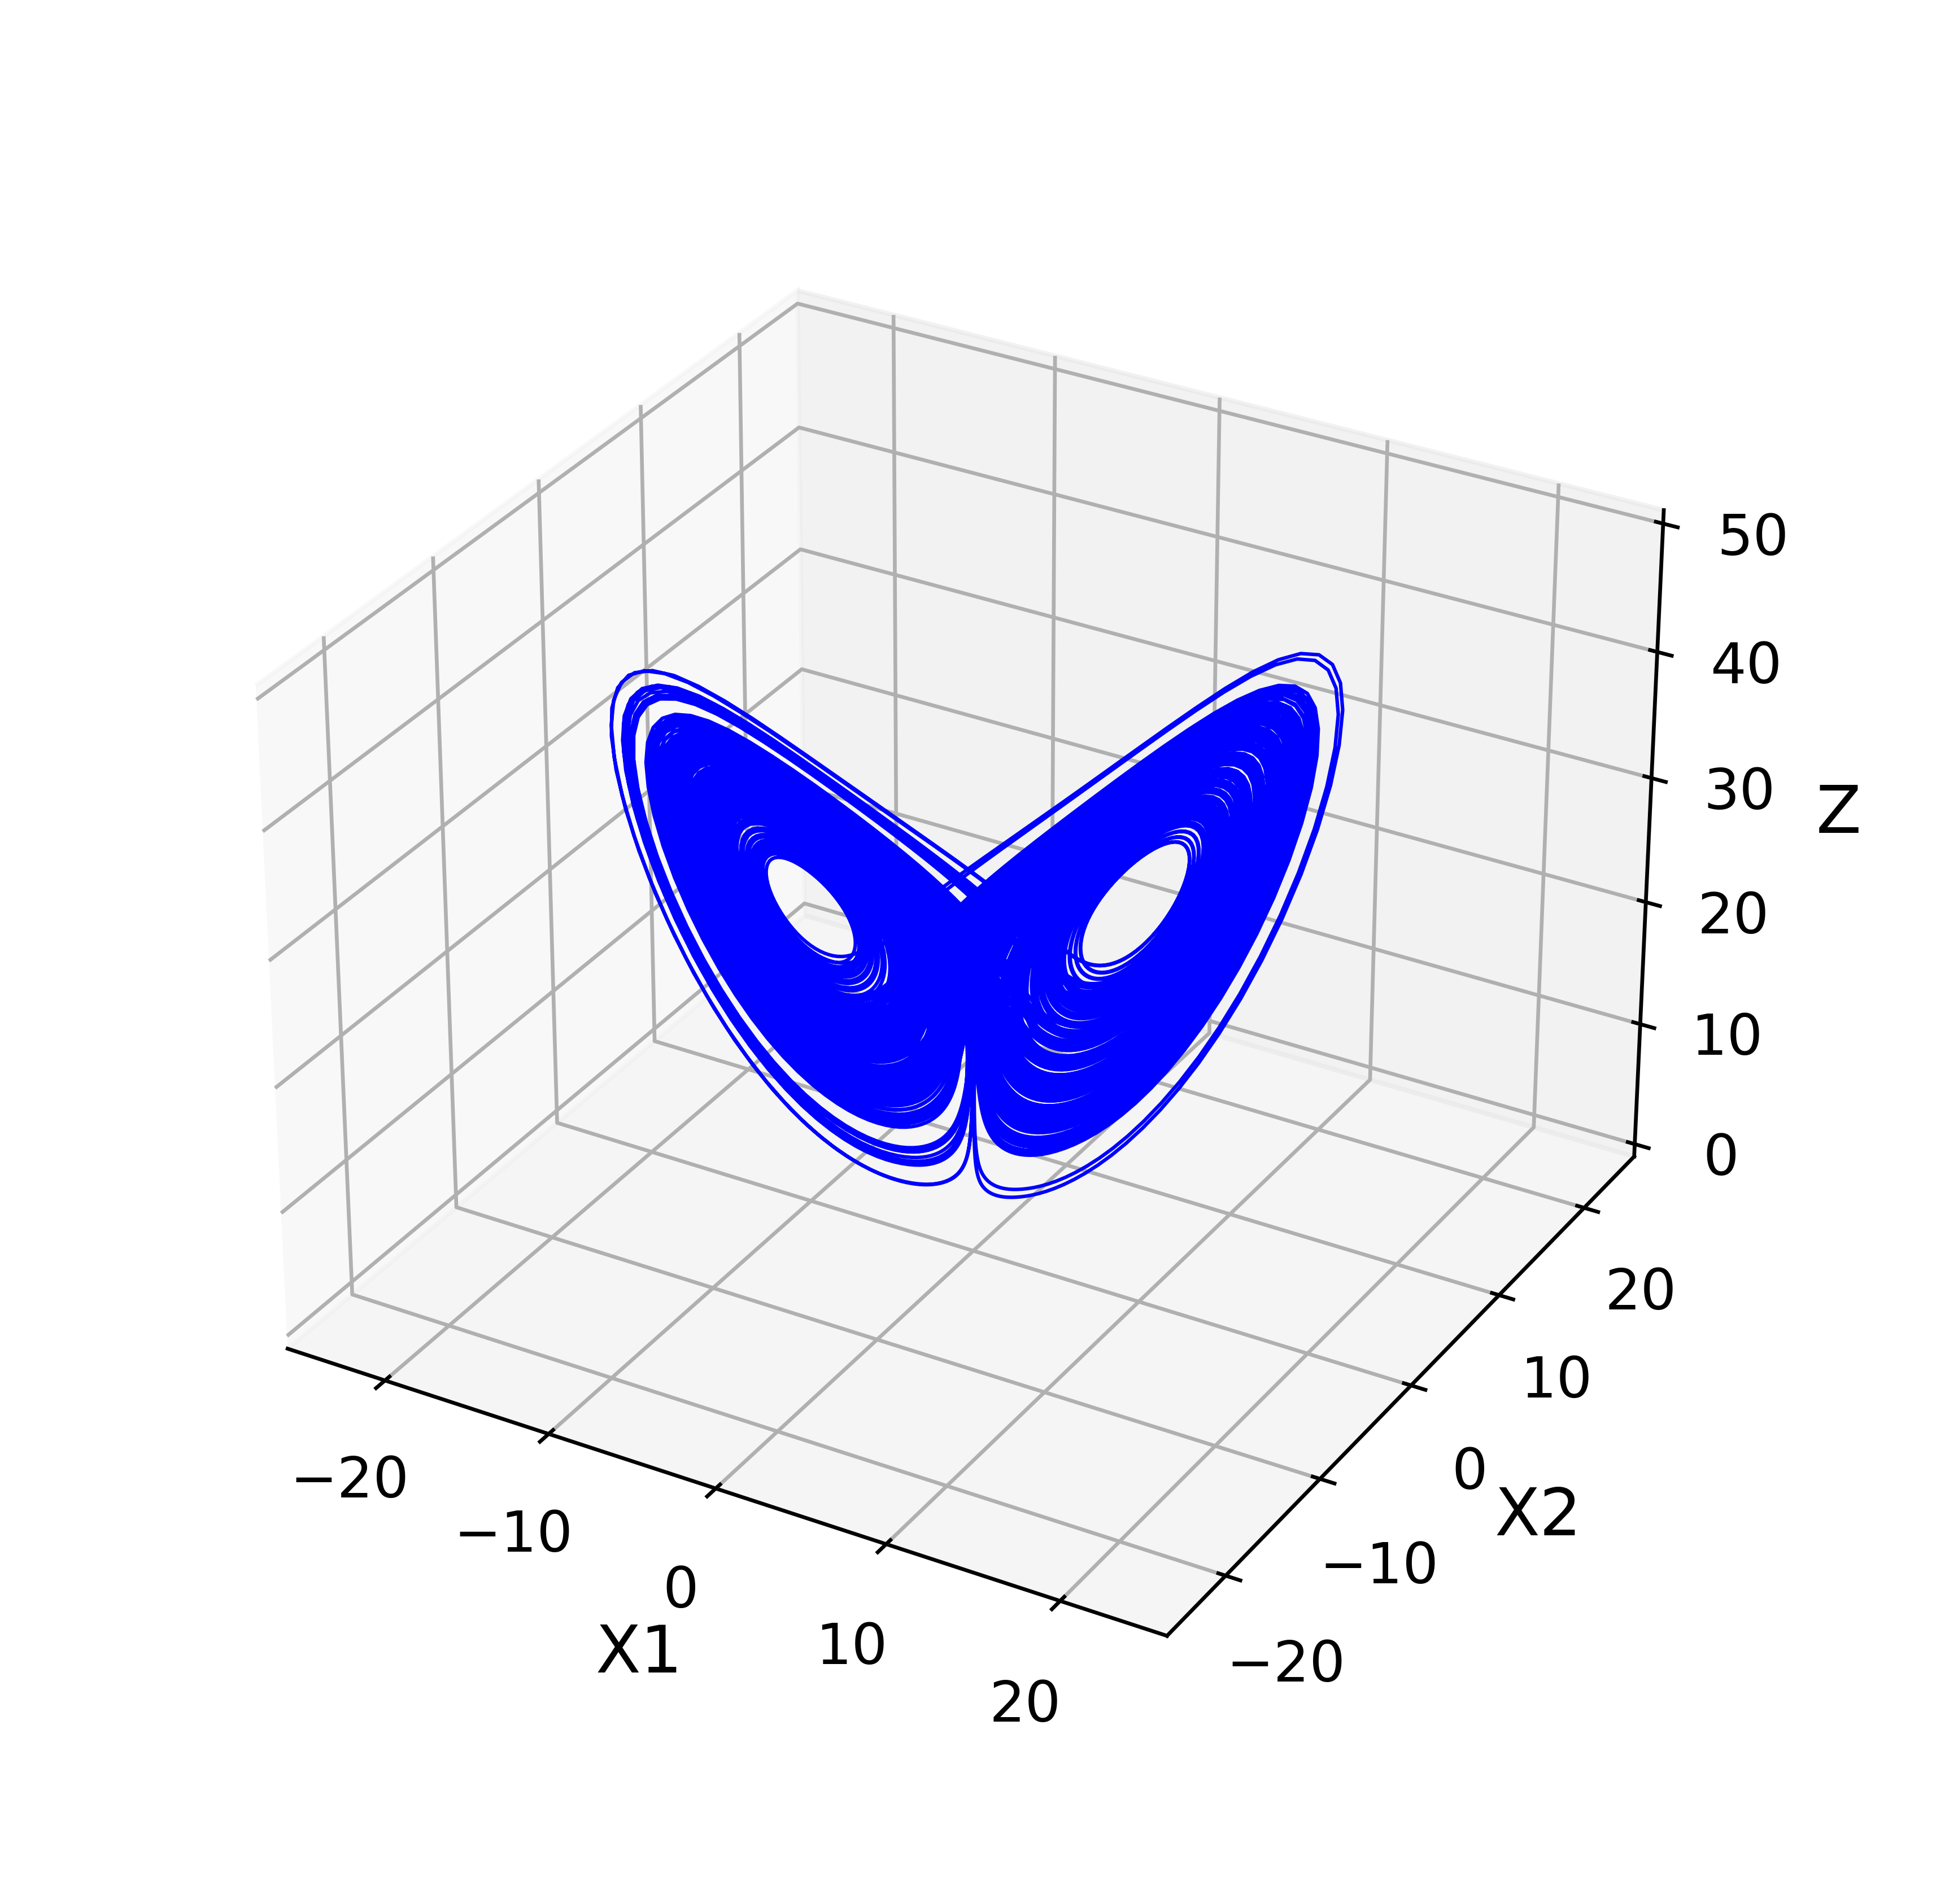
\includegraphics[width=\textwidth]{media/extendedattractor_seed_50.png}
		\caption{}
		\label{fig:sub2}
	\end{subfigure}
	\hfill
	\begin{subfigure}[b]{0.495\textwidth}
		\centering
		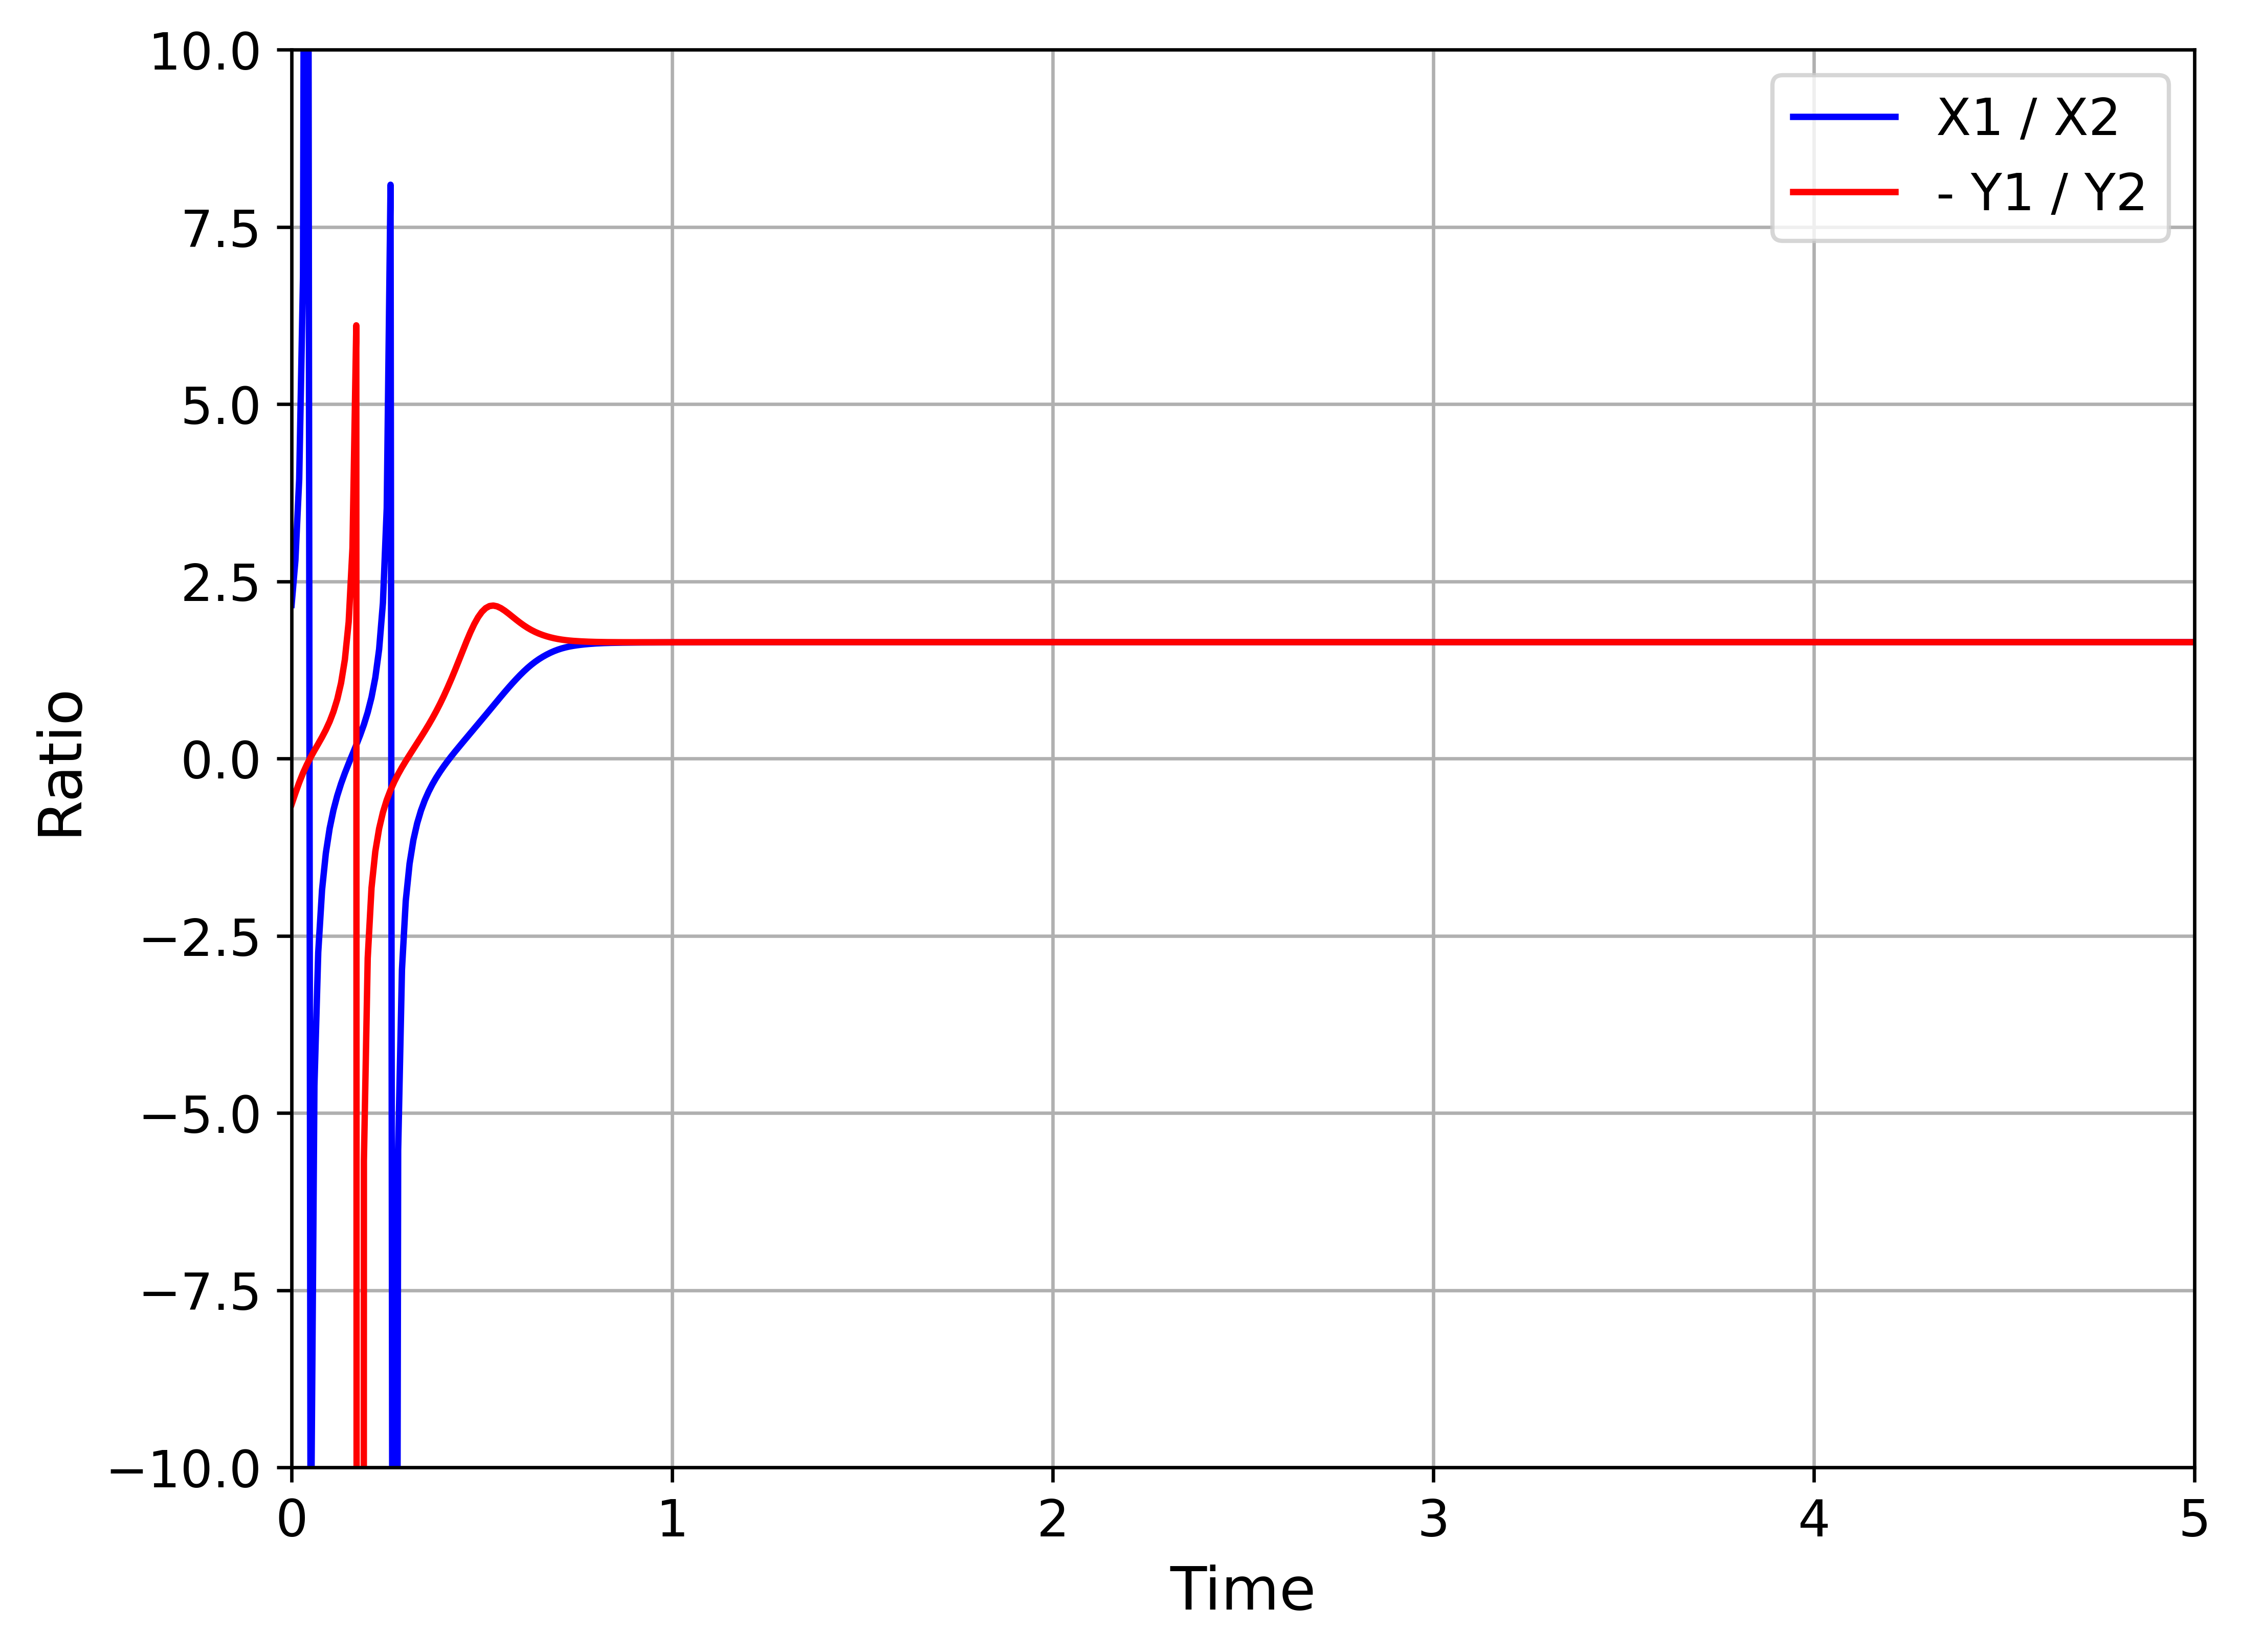
\includegraphics[width=\textwidth]{media/X1_X2_Y1_Y2_vs_time_seed_50.png}
		\caption{}
		\label{fig:sub2}
	\end{subfigure}
		\hfill
	\begin{subfigure}[b]{0.495\textwidth}
		\centering
		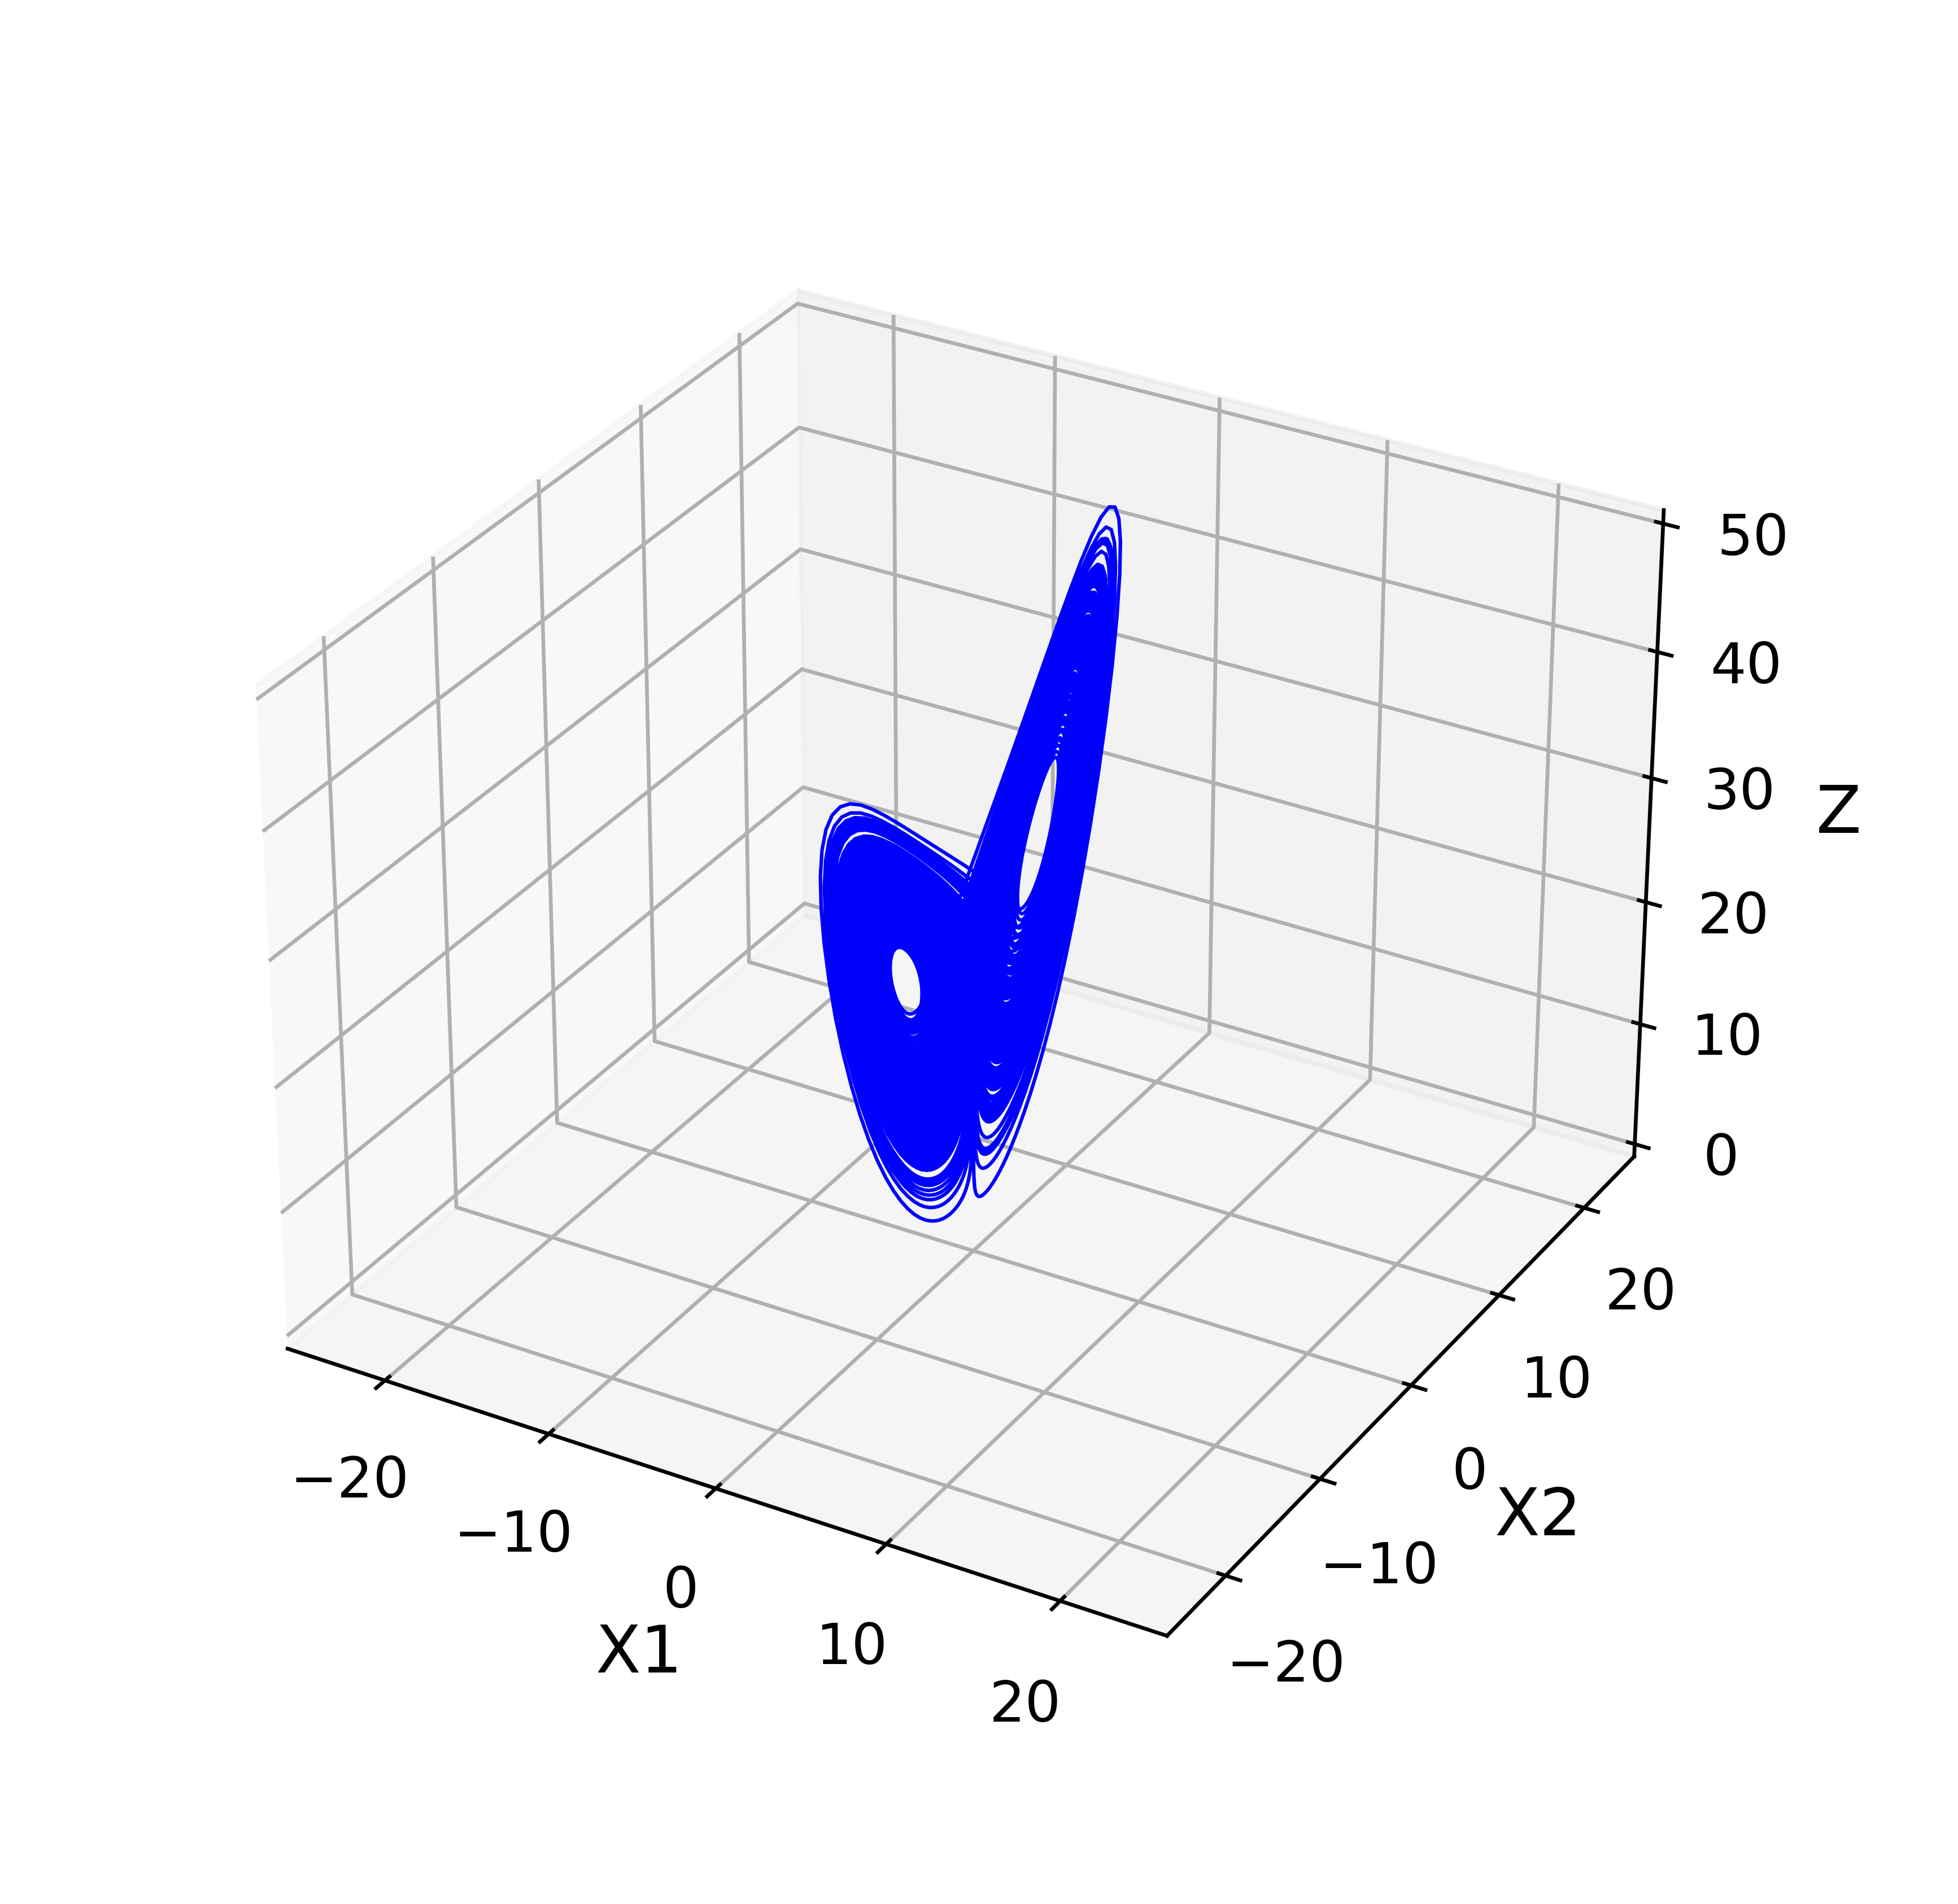
\includegraphics[width=\textwidth]{media/extendedattractor_seed_45.png}
		\caption{}
		\label{fig:sub2}
	\end{subfigure}
	\hfill
	\begin{subfigure}[b]{0.495\textwidth}
		\centering
		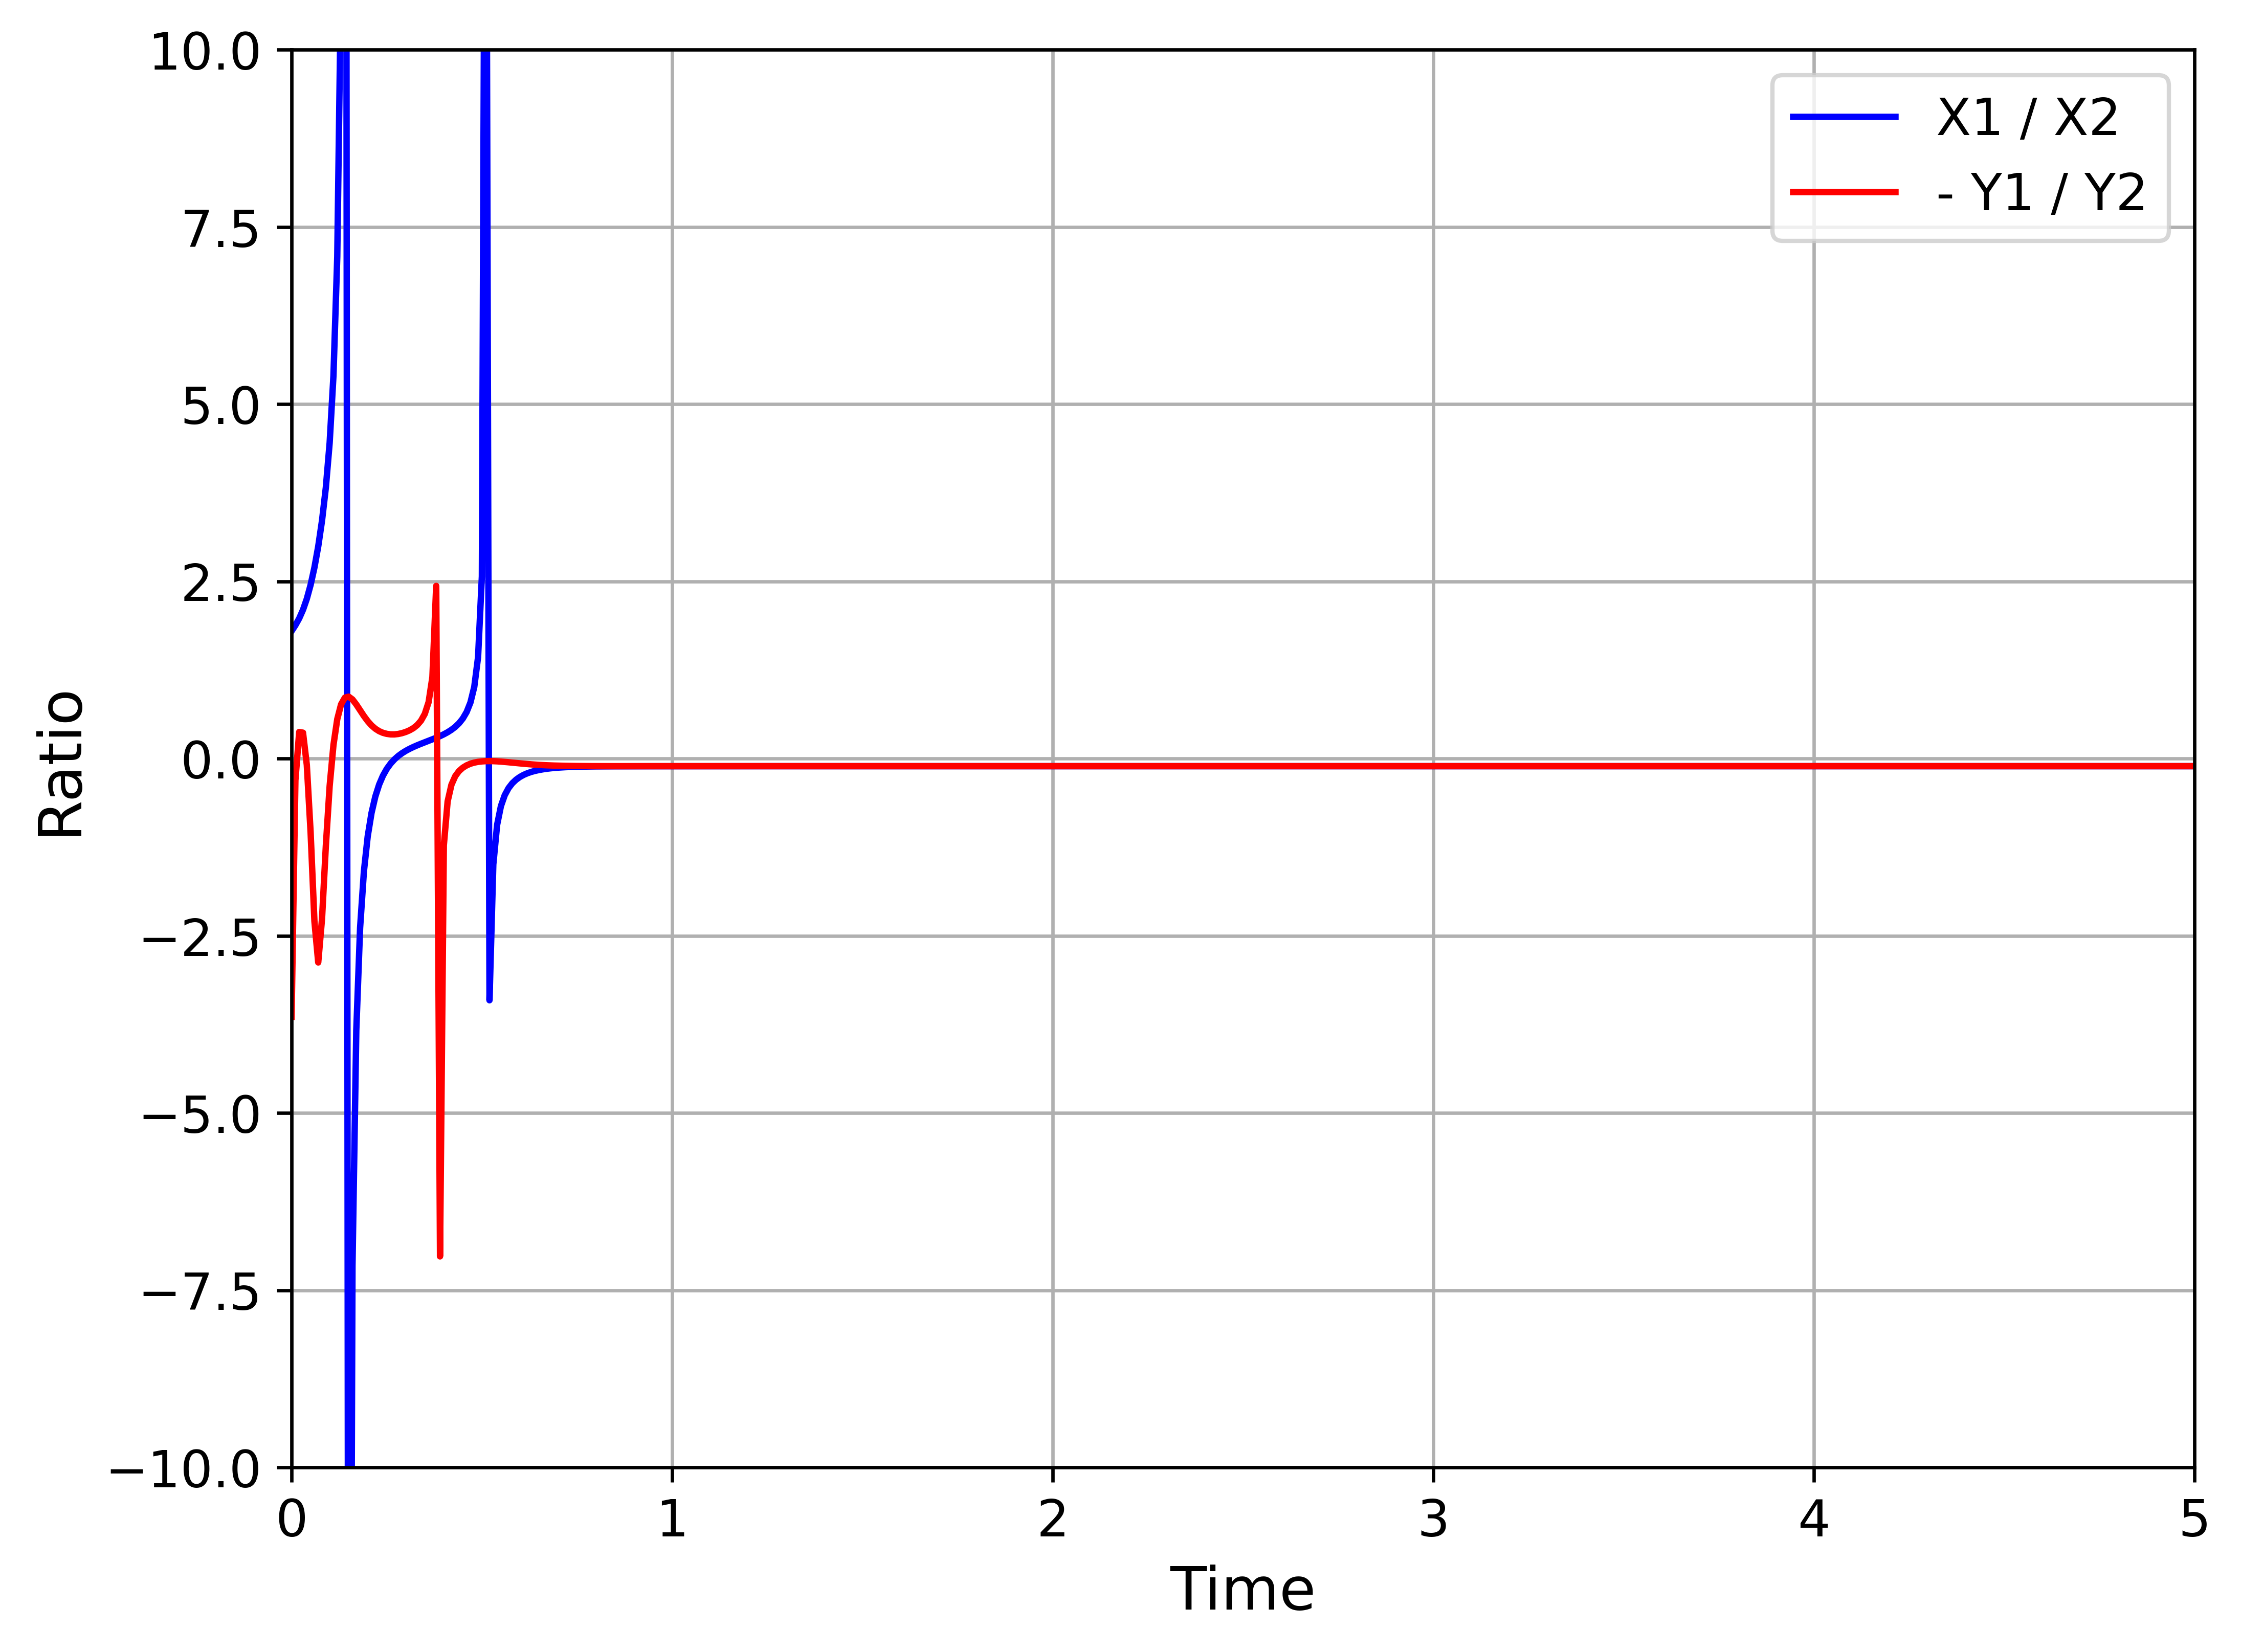
\includegraphics[width=\textwidth]{media/X1_X2_Y1_Y2_vs_time_seed_45.png}
		\caption{}
		\label{fig:sub2}
	\end{subfigure}
	
	\caption{(a and c) Trajectories of the extended Lorenz system in the $X_1-X_2-Z$ space for two different initial conditions, at $r=28$. (b and d) Corresponding time evolution of the ratios $X_1/X_2$ and $-Y_1/Y_2$.}
	\label{fig:extendedsimulations}
\end{figure}

\section{Conclusions}

This work explored the dynamics of Rayleigh-Bénard convection through reduced-order modeling approaches, highlighting the rich nonlinear behavior that emerges even in low-dimensional representations of the system. Our investigation began with a linear stability analysis of the Boussinesq equations, which established the critical Rayleigh number $\text{Ra}_{\text{cr}} = 657.5$ for the onset of convection. Beyond this threshold, the motionless conductive state becomes unstable, giving rise to convective motion.\\

The classical Lorenz system, derived from a three-mode Galerkin truncation, provided significant insights into the nonlinear regime of the convection problem. Our bifurcation analysis revealed three distinct dynamical regimes as the Rayleigh number increases:

\begin{enumerate}
	\item For $r < 1$ (Ra $<$ Ra$_{\text{cr}}$), the system has a single stable fixed point representing the motionless conductive state.
	\item For $1 < r < 24.74$, two symmetric stable fixed points emerge through a supercritical pitchfork bifurcation, corresponding to steady convective rolls with opposite senses of rotation.
	\item For $r > 24.74$, the system transitions to chaotic behavior via a subcritical Hopf bifurcation, characterized by the famous butterfly-shaped strange attractor.
\end{enumerate}

\noindent The Lorenz system also exhibited metastable chaos in the parameter range $13.926 < r < 24.74$, where trajectories display transient chaotic behavior before eventually settling into one of the stable fixed points.\\

While the Lorenz model successfully captures many key features of convective dynamics, it breaks an important symmetry inherent in the original problem: translational invariance in the horizontal direction. To address this limitation, we implemented the five-mode truncation model proposed by Chen and Price, which preserves this critical symmetry. The extended system revealed that the fixed points form a continuous circle in phase space rather than isolated points, reflecting the freedom to translate the convection pattern horizontally.\\

The geometry of the strange attractor in the extended system is particularly illuminating. We demonstrated that the extended system contains a continuous family of invariant subsets, each equivalent to the Lorenz system, and that trajectories rapidly converge to one of these subsets depending on initial conditions. Geometrically, the Lorenz attractor is a cross-section of the attractor of the extended five-dimensional system, revealing how the original three-dimensional model provides only a slice of the complete solution space in the convection problem.
\\

This study shows how even low-dimensional models can capture essential aspects of complex fluid dynamical systems. The progression from linear stability analysis to increasingly sophisticated nonlinear reduced-order models offers a template for addressing other hydrodynamic stability problems. The connection between the Lorenz system and its extended counterpart also highlights how symmetry considerations affect the structure of attractors in dynamical systems.

\section*{Appendix: Code Availability}
The code used for all simulations and visualizations presented in this report is available at: \\
\url{https://github.com/shubhranil04/ExtendedLorenzSystem.git}

\bibliographystyle{unsrt}
\bibliography{references}


\end{document}